% !TEX encoding = UTF-8 Unicode
%%%%%%%%%%%%%%%%%%%%%%%%%%%%%%%%%%%%%%%%%%%%%%%%%%%%%%%%%%%%%%%%%%%%%%%%%%%%%%%%%%%%%%%%%%%%%%%%%%%%%%%%%
%% 
%%  This file is asmejour-template.tex, a template to format papers in the style of ASME journal papers. 
%%
%%  This file is version 1.18 dated 2022/01/10
%%
%%  Author: John H. Lienhard V
%%          Department of Mechanical Engineering
%%          Massachusetts Institute of Technology
%%          Cambridge, MA 02139-4307 USA
%%
%%  Class options include:
%%
%%          * Option to color the vertical bar in the title block [barcolor = colorname] 
%%          *    where colorname is any name def'd by xcolor package; omit barcolor option to get black
%%
%%          * Option to omit the list of figures and list of tables at the end [nolists]
%%
%%          * Math options from M. Sharpe's newtxmath package: upright integrals [upint];
%%          *    [varvw] for a v and w that are better distinguished from Greek nu; [subscriptcorrection]
%%			*	 to fine-tune the placement of math subscripts; and also additional options such as
%%          *    [smallerops, varg, slantedGreek, frenchmath, varbb, cmbraces]. Version 1.6 or higher
%%          *    is recommended.
%%
%%          * Option to include line numbers [lineno]. The lineno package does not number tables, 
%%          *    footnotes, captions, etc. You must run *twice* for proper placement of the numbers. 
%%          *    This option will disable balancing of the column heights on final page.
%%
%%			* Option to balance column heights on final page [balance]. This option sometimes
%%			*    misbehaves, so use it with an awareness that it can create unexpected problems.
%%			*	 This option is not compatible with line numbering.
%%
%%          * Options for copyright notices:
%%			* 	 Omit the ASME copyright from the footer [nocopyright]
%%			*	 Copyright footnote if all authors are government employees  [govt]
%%			*	 Copyright footnote if some authors are government employees [govtsome]
%%			*	 Copyright footnote for government contractors [contractor]
%%
%%          * Option to omit all ASME text fields from the footer [nofoot].
%%
%%			* Options for PDF/A compliance. [pdf-a] will produce PDF/A-3u compliance with sRGB OutputIntent.
%%			*	 [pdfapart= 1 or 2 or 3] and [pdfaconformance= b or u] can enable levels 1b, 2b, 2u, and 3b.
%%			*
%%			*    The most recent versions of LaTeX (2021 and later) are moving toward integrated support for pdf-a, 
%%			*    through \DeclareDocumentMetadata{..}. The asmeconf class supports these new features, which can 
%%			*	 replace the aforementioned class options. (An up-to-date LaTeX installation is required.)
%%
%%          * Many options for calligraphic, script, and fraktur fonts from the mathalfa package; the
%%          *    example value used is: mathalfa=cal=euler (use Euler font for \mathcal)
%%          *    some other options for cal are: dutchcal, zapfc, cm (default), boondox,...
%%          *    frak (fraktur), bb (blackboard bold), scr (script) may also be controlled.
%%
%%          * An option to use newtxtext's superiors font for footnotes [nodefaultsups] and an option
%%          *    for slightly larger small capitals [largesc]
%%
%%          * Options for typewriter font 
%%          *    [hyphenate] allow hyphenation (normally suppressed because for typewriter font is often used for code)
%%			*	 [var0] replace default slashed zero by unslashed zero
%%			*	 [mono] force interword separation to monospacing
%%
%%          * Options for the babel package to support passages in other languages (such as a translated 
%%          *    abstract in an appendix), e.g. [french].  The main language will default to English 
%%          *    unless a different main language is selected, e.g. [main=spanish]. See Appendix C for details.
%%
%%  For details of the newtx and mathalfa packages, refer to their documentation (available at CTAN: http://ctan.org).
%%
%%  The use of commands defined or modified by the asmejour class is illustrated below. In particular, some care
%%  is needed when using complicated math and macros in section headings, to avoid problems with pdf bookmarks, 
%%  as facilitated by the optional argument of \section (also illustrated below).
%%
 %=========================================================
%% 
%% LICENSE: 
%%
%% Copyright (c) 2022 John H. Lienhard
%%
%% Offered under the MIT license: https://ctan.org/license/mit 
%%
%%%%%%%%%%%%%%%%%%%%%%%%%%%%%%%%%%%%%%%%%%%%%%%%%%%%%%%%%%%%%%%%%%%%%%%%%%%%%%%%%%%%%%%%%%%%%%%%%%%%%%%%%

%% Class options are described above.
\documentclass[10pt,subscriptcorrection,upint,varvw,barcolor=Goldenrod3,mathalfa=cal=euler,balance,hyphenate,french,pdf-a, nolists,nofoot]  %% To omit final list of figures and tables, use the class option [nolists]
{asmejour} %
\usepackage{float,newtxtext,newtxmath}
\usepackage{caption}
\usepackage[switch]{lineno}


\captionsetup[figure]{font=scriptsize}

%%%%  pdf metadata  %%%%%%%%%%%%%%%%%%%%%%%%%%%%%%%%%%%%%%%%%%%%%%%%%%%%%%%%%%%%%%%%%%%%%%%%%%%%%%%%%%%

\hypersetup{%
	pdfauthor={Paulina Rodriguez}, 
	pdftitle={EDDS Verification Manuscript},                  	% <=== 
	pdfkeywords={EDDS, medical device, verification, computational model, code verification, solution verification},
	pdfsubject = {This study is assessing the verification studies of the EDDS medical device computational model study},
}

%%%%  Journal name and optional copyright year %%%%%%%%%%%%%%

%% Omit "Journal of". If Journal Name is quite long, use \\ to insert a line break
%% Add this once we decide on the journal
%% \JourName{Heat Transfer} %<=== change to the name of your journal

%% The default copyright year is the current year
%% \PaperYear{2022} sets 2022; and \PaperYear{} omits the year entirely.
                   
%%%%  end of preamble  %%%%%%%%%%%%%%%%%%%%%%%%%%%%%%%%%%%%%%%%%%%%%%%%%%%%%%%%%%%%%%%%%%%%%%%%%%%%%%%%%

\begin{document}
\modulolinenumbers[2]
\linenumbers
% Change to your author name[s] and addresses, in the desired order of authors.
% First name, middle initial, last name
% Use title case (upper and lower case letters)
% Note usage below for corresponding author.

\SetAuthorBlock{Paulina Rodriguez}{Department of Mechanical and Aerospace Engineering,\\
   The George Washington University} %\\
   %Street address,\\
   %City, State, Country \\
   %email: xxx@yyy.zzz} 
\SetAuthorBlock{Lorena Barba}{Department of Mechanical and Aerospace Engineering,\\
   The George Washington University,}
\SetAuthorBlock{Brian Carnes}{Sandia National Laboratories}
\SetAuthorBlock{Matthew Myers}{Puente Translational Sciences}

% To label one or more corresponding authors put "Name\CorrespondingAuthor". No space after "Name".
% An optional argument can be added if email is not in address block as
%      "Name\CorrespondingAuthor{write@to.me}"
% Can also include multiple emails and use the command more than once for multiple corresponding authors,
%      "Name\CorrespondingAuthor{write@to.him, write@to.her}"

%\SetAuthorBlock{John H.\ Lienhard V\CorrespondingAuthor}{%
%Fellow ASME\\
%Rohsenow Kendall Heat Transfer Laboratory, \\
%Department of Mechanical Engineering,\\
%Massachusetts Institute of Technology, \\
%Cambridge, MA 02139 USA \\
%email: lienhard@mit.edu
%}

%%% Change to your paper title. Can insert line breaks if you wish (otherwise breaks are selected automatically).
\title{Verification of a Conjugate Heat Transfer Model in OpenFOAM for a Simplified Medical Device Geometry}


%%% Change these to your keywords.  Keywords are automatically printed at the end of the abstract.
%%% This command must come BEFORE the end of the abstract.
%%% If you don't want keywords, omit the \keyword{..} command.
% \keywords{Verification, Code Verification, Solution Verification, Conjugate Heat Transfer, OpenFOAM, Computational Modeling, Medical Device, V\&V 40, Model Credibility, }
\keywords{verification and validation, solution verification, conjugate heat transfer, computational fluid dynamics, medical device modeling, model credibility, reproducibility, discretization error, OpenFOAM, V\&V 40}

% Abstract
\begin{abstract}
    %% Abstract should be no more than 250 words
% This study presents a rigorous verification effort for a computational model of a simplified medical device geometry involving conjugate heat transfer. Using the open-source \texttt{chtMultiRegionFoam} solver in OpenFOAM, both code and solution verification activities were performed to establish the model’s numerical accuracy and trustworthiness prior to validation. Code verification was carried out using benchmarks: Hagen–Poiseuille flow for laminar momentum transport and solid conduction. In both cases, the numerical results closely matched analytical solutions. Solution verification included systematic studies of mesh resolution, timestep size, and solver tolerance. Spatial and temporal errors were quantified using an extrapolated value computed using StREEQ to generate relative error measures, with observed convergence behavior supporting the selection of a configuration that balances computational cost and accuracy. The modeling effort aligns with the ASME V\&V 40 standard and follows a risk-informed credibility framework suitable for medium to low risk applications. This work provides a transparent and reproducible case study in model verification for computational modeling and simulation 
% (CM\&S) in medical device applications. The results provide a foundation for subsequent validation and uncertainty quantification, contributing to the broader goal of establishing credible simulation-based evidence.

Computational models and simulations (CM\&S) are increasingly used in medical device development, yet their adoption in regulatory decision-making remains limited due to challenges in establishing model credibility. This study presents a structured and reproducible verification framework for a computational model of a simplified medical device involving conjugate heat transfer using \texttt{OpenFOAM}'s \texttt{chtMultiRegionFoam} solver. Code verification is performed using analytical benchmarks for laminar pipe flow, radial heat conduction, and transient thermal diffusion yielding observed orders of convergence of $p=1.95$, $p=2.08$, and $p=2.15$ (at 0.025 s) respectively. Solution verification evaluates discretization error through systematic mesh and timestep refinement and regression-based extrapolation using the \texttt{StREEQ} method. Results show that spatial and temporal discretization errors in transient coupled simulations interact and cannot be assessed independently. Co-refinement is required to capture true convergence behavior, while independent refinement yields polluted convergence rates. Computational cost analysis demonstrates diminishing returns with refinement and highlights that runtime does not vary monotonically with discretization parameters due to solver convergence behavior. The use of a simplified geometry enables rigorous verification while retaining the dominant physics of the system. Grounded in a risk-informed framework consistent with ASME V\&V 40 Standard, this study demonstrates that a level of verification rigor beyond minimal practice can be achieved through targeted model simplification and systematic analysis under realistic computational constraints.
\end{abstract} 

% \date{Version \versionno, \today}%% You can modify this information as desired. 
							%% Putting \date{} will suppress any date.  
							%% If this command is omitted, date defaults to \today
							%% This command must come somewhere before \maketitle

\maketitle %% This command creates the author/title/abstract block. Essential!

%%%%%%%%%%%%%%%%%%%%%%%%%%%%%%%%%%%%%%%%%%%%%%%%%%%%%%%%%%%%%%%%%%%%%%%%%%%%%%%%%%%%%%%%%%%%%%%%%%%%%%%
%%%%%%%%%%%%%%%%%%%%%  End of fields to be completed. Now write! %%%%%%%%%%%%%%%%%%%%%%%%%%%%%%%%%%%%%%


% % Main sections
\section{Introduction}
% Section Introduction
Computational models and simulations (CM\&S) are increasingly used across the medical device lifecycle, from early stages in design to optimization of in silico testing and post-market surveillance \cite{morrisonFrontiers}. These tools offer cost-effective, flexible, and scalable alternatives to traditional experimentation. However, their use in high risk regulatory decision making remains limited \cite{fda_credibility_program, fda2022Success}. To be accepted by regulatory agencies such as the U.S. Food and Drug Administration (FDA), computational models must be supported by rigorous, transparent evidence demonstrating that they are appropriate for their use case and capable of producing trustworthy results. 

Establishing this trust is particularly challenging for systems involving multiphysics interactions, coupled domains, and inherent uncertainties, especially when experimental data are sparse, costly, or difficult to obtain. In such settings, verification, validation, and uncertainty quantification (VVUQ) are essential. However, the required level of rigor must be aligned with the model’s intended use and associated risk. For medium to low risk applications, comprehensive experimental studies or high-fidelity simulations may be impractical. In these cases, credibility depends not only on numerical rigor but also on transparency, including clearly communicating assumptions, limitations, and modeling decisions to support risk-informed interpretation.

To provide context for the level of verification performed, this study adopts a risk-informed perspective consistent with the ASME V\&V 40 framework. For the present application, the model is characterized by a low decision consequence and moderate model influence, corresponding to a medium–low risk classification. Under this classification, a moderate to minimal level of verification would typically be sufficient. However, in this work, additional rigor is pursued where computationally feasible. In particular, simplified geometries and isolated physical configurations are used to enable more detailed assessment of numerical behavior, including estimation of discretization error and evaluation of observed order of accuracy. This approach provides a level of verification beyond minimal while remaining practical.

This study focuses specifically on verification as a foundational component of the VVUQ process, with validation and uncertainty quantification addressed in a subsequent companion study. In particular, this study presents a structured and transparent verification study of a computational model for a medical device application involving heated internal flow. The system is modeled as a conjugate heat transfer (CHT) problem, where laminar fluid flows through a heated solid casing and exchanges thermal energy before exiting the device. Simulations are performed using the open-source finite volume solver \texttt{OpenFOAM}, specifically the \texttt{chtMultiRegionFoam} solver for coupled fluid-solid heat transfer  \cite{openfoamSolvers, chtMultiRegion}.

The verification approach focuses on both code and solution verification to establish numerical correctness and quantify discretization error. This includes the use of analytical problems, systematic mesh and timestep refinement studies, and regression-based error estimation. Particular emphasis is placed on transient, coupled configurations, where spatial and temporal resolution interact and cannot be assessed independently.

This work is grounded in the ASME V\&V 40 framework for credibility assessment in medical device applications and aligns with FDA-recognized standards, including V\&V 10, V\&V 20, and V\&V 40 \cite{vv10, vv20, vv40, pathmanathanAA, vv10_fdarecognized, vv20_fdarecognized, vv40_fdarecognized, fda_guidance_2023}. While these standards define high-level credibility principles, they do not prescribe specific verification workflows. To address this gap, the methodology presented here draws on best practices from high-consequence fields such as aerospace and nuclear engineering, where VVUQ processes are well established due to similar experimental and modeling constraints \cite{OberkampfRoy2013, Roache2009, AIAA-G-077-1998}. Additional details on the risk-informed credibility assessment, including V\&V 40 gradation selection and justification, are provided in publicly accessible repository materials \cite{edds_credibility_repo}.


By openly documenting simulation workflows, input files, and post-processing procedures, this study provides a reproducible case study in verification for medical device modeling. The goal is to demonstrate how rigorous, transparent, and risk-informed verification can be achieved within realistic computational and resource constraints, supporting broader adoption of CM\&S in regulatory and engineering applications.

\section{Methods}
This study is motivated by a heat transfer driven electronic drug delivery system (EDDS) medical device, which uses applied power to heat fluid flowing through the device and into a user's mouth cavity. While the full system includes complex components such as coils for heating and an expanding mouthpiece, verifying the entire system limits the level of rigor achievable in code and solution verification due to geometric and multiphysics complexity. 

To enable systematic verification, a simplified geometry is adopted that preserves the dominant transport mechanisms of laminar flow and conjugate heat transfer while minimizing geometric complexity. This reduction enables direct comparison to analytical solutions and supports high-resolution studies. By verifying key physical processes in isolation, this approach establishes confidence in the numerical modeling framework and provides a foundation for progressively reintroducing complexity in future validation and application studies.

\subsection{Verification Framework}
Verification is divided into two categories: \textit{code verification}, which assesses the correctness of the numerical implementation through comparison with analytical solutions, and \textit{solution verification}, which quantifies numerical uncertainty arising from spatial and temporal discretizations, solver settings, and modeling assumptions. These activities follow the framework outlined in ASME V\&V 20 and V\&V 40 \cite{vv20,vv40}, and support a structured credibility assessment of simulation results for subsequent validation and decision-making.

To isolate sources of numerical error, each verification component is further subdivided according to the underlying physical processes and modeling complexity. Code verification is performed using three cases: hydrodynamic flow, radial heat conduction, and transient thermal diffusion, which independently assess the solver’s ability to reproduce fluid transport, steady thermal transport, and transient heat transfer across the fluid-solid interface. 

Solution verification is conducted using coupled fluid and thermal configurations which increase in complexity. These include a steady-state coupled pipe model and a transient, device-representative EDDS configuration. The latter provides the closest approximation to the target medical device and enables evaluation of numerical uncertainty under application relevant conditions.

\subsection{System Description \& Operating Conditions}
The pipe system is designed to approximate the geometry of the medical device, including both the internal fluid channel and surrounding casing. The fluid domain is partitioned into three regions: the pipe inlet, the pipe case, and the pipe outlet. The central pipe section, shown in Figure~\ref{fig:geometry-schematic-gen}, is thermally coupled to a surrounding solid domain representing the casing, within which volumetric heat generation is applied.

\begin{figure}[ht]
    \centering
    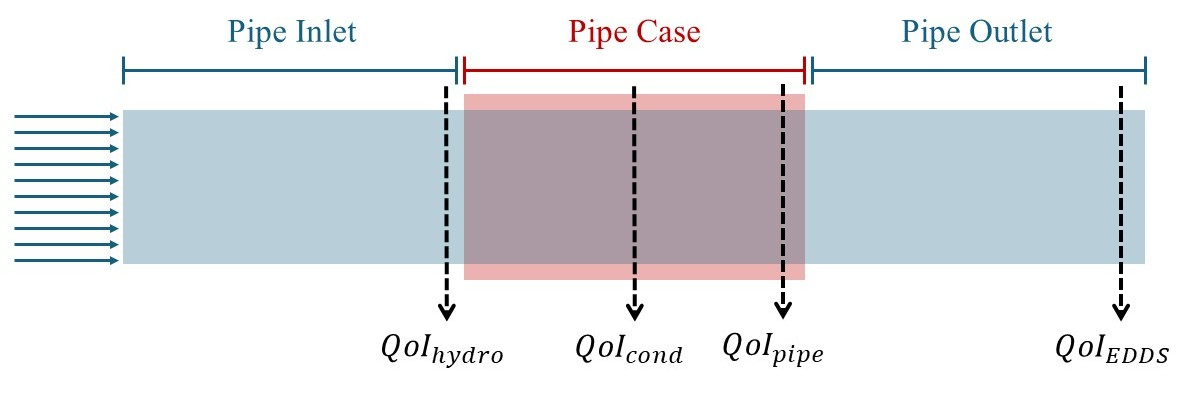
\includegraphics[width=\linewidth]{figures/schematic/schematics_verifedds_v2.jpg}
    \caption{Schematic of the generalized pipe configuration used across all verification studies.}
    \label{fig:geometry-schematic-gen}
\end{figure}

The pipe has an internal diameter of 4.54~mm and is surrounded by a casing with a thickness of 0.30~mm. Operating conditions impose a total heating power of 1~W, applied uniformly as a volumetric heat source within the casing for a duration of 10~seconds. The fluid enters with a uniform velocity of 0.5~m/s and an inlet temperature of 26.85$^\circ$C (300~K), resulting in a laminar, transient conjugate heat transfer problem involving coupled solid-fluid thermal interactions.

All verification studies introduce controlled variations in geometry, temporal regime, and quantities of interest, as summarized in Table~\ref{tab:geometry_qty}. For code verification, the configuration is intentionally simplified to isolate numerical behavior and enable comparison with analytical solutions. A sufficiently long pipe is employed to ensure fully developed hydrodynamic and thermal conditions, thereby minimizing inlet and outlet effects. 

% \begin{table*}[htbp]
%     \centering
%       \caption{Geometry quantities, in mm, for the code and solution verification studies. The pipe diameter is 4.54 mm and the case thickness is 0.30 mm.}
%     \begin{tabular}{llll|ccccc}\toprule
%               Model& Verification Study
%  &Regime&Geometry&pipe inlet&pipe case&pipe outlet& pipe &  case \\\midrule
%               Hydrodynamic& Code
%  &Steady&long pipe&45&45&0&90& 
%      45\\
%   Radial Conduction & Code
%  &Steady&medium pipe&11.375& 45& 0& 56.25& 45\\
%   Thermal Diffusion & Code
%  &Transient&medium pipe&11.375& 45& 0& 56.25& 45\\
%   Coupled Pipe& Solution
%  &Steady &long pipe&45& 45& 0& 90& 45\\
%   Simplified EDDS& Solution &Transient&short pipe&2.021& 7.2& 42.509& 51.73& 7.2\\ \bottomrule\end{tabular}
  
%     \label{tab:geometry_qty}
% \end{table*}

\begin{table*}[htbp]
    \centering
    \caption{Geometric quantities for the code and solution verification studies. All dimensions are reported in mm. The pipe diameter is 4.54 mm, and the case thickness is 0.3 mm. \(L_{\mathrm{in}}\), \(L_{\mathrm{case}}\), and \(L_{\mathrm{out}}\) denote the pipe inlet, pipe case, and pipe outlet lengths, respectively, and \(L\) denotes the total pipe length.}
    \begin{tabular}{p{2.4cm}p{1.25cm}p{1.2cm}p{1.5cm}p{3.5cm}p{3.6cm}}
        \toprule
        Study & Verification & Regime & Geometry & Physical configuration & QoI \\
        \midrule        
        Hydrodynamic
        & Code
        & Steady
        & $L_{\mathrm{in}}=45$
          $L_{\mathrm{case}}=45$ 
          $L_{\mathrm{out}}=0$
          $L=90$ 
        & Fluid only; 
          $U=0.5$ m/s;
          $p=101.325$ kPa;
        & 
          $QoI_{\mathrm{hydro}}$: Axial velocity \\
        
        \midrule
        Radial conduction
        & Code
        & Steady
        & $L_{\mathrm{in}}=11.375$
          $L_{\mathrm{case}}=56.375$ 
          $L_{\mathrm{out}}=0$
          $L=56.25$
        & Solid conduction only; Uniform heat source $S_E=3.5\times10^{8}$~W/m$^3$ &  
          $QoI_{\mathrm{cond}}$: Radial temperature solid \\
        
        \midrule
        Thermal diffusion
        & Code
        & Transient
        & $L_{\mathrm{in}}=11.375$
          $L_{\mathrm{case}}=56.375$
          $L_{\mathrm{out}}=0$
          $L=56.25$
        & Transient thermal diffusion;
          Fluid $T_0=20^\circ$C;
          Solid $T_0=30^\circ$C;
        & 
          $QoI_{\mathrm{diff}}$: Radial temperature fluid \\
        
        \midrule
        Coupled pipe
        & Solution
        & Steady
        & $L_{\mathrm{in}}=45$
          $L_{\mathrm{case}}=45$
          $L_{\mathrm{out}}=0$
          $L=90$
        & Steady conjugate heat transfer;
          $U_{\mathrm{in}}=0.5$ m/s;
          $p_{\mathrm{out}}=101.325$ kPa;
          $T_{\text{solid}}=50^\circ$C.
        & 
          $QoI_{\mathrm{pipe}}$: Bulk fluid temperature \\
        
        \midrule
        Simplified EDDS
        & Solution
        & Transient
        & $L_{\mathrm{in}}=2.021$
          $L_{\mathrm{case}}=7.2$
          $L_{\mathrm{out}}=42.509$
          $L=51.730$
        & Transient conjugate heat transfer;
          $U_{\mathrm{in}}=0.5$ m/s;
          $T_{\mathrm{in}}=26.85^\circ$C (300~K);
          $p_{\mathrm{out}}=101.325$ kPa;
          volumetric heat source applied to casing.
        &  $QoI_{\mathrm{EDDS}}$: Cross-sectional average temperature \\
        
        \bottomrule
    \end{tabular}
    \label{tab:geometry_qty}
\end{table*}


To achieve this, the pipe length is selected to exceed both the hydrodynamic and thermal entry lengths, given by

% \begin{equation}
% \small
% L_{\text{hydro}} = 0.05\,Re\,D \approx 35~\text{mm}, \quad
% L_{\text{therm}} = 0.05\,Re\,Pr\,D \approx 25~\text{mm}
% \end{equation}
\begin{equation}
\begin{aligned}
L_{\mathrm{hydro}} &= 0.05\,Re\,D \approx 35~\mathrm{mm}, \\
L_{\mathrm{therm}} &= 0.05\,Re\,Pr\,D \approx 25~\mathrm{mm},
\end{aligned}
\end{equation}
where $Re$ is the Reynolds number, $Pr$ is the Prandtl number, and $D$ is the pipe diameter. These conditions ensure fully developed flow and thermal fields and support rigorous assessment of discretization accuracy under steady-state assumptions.

In contrast, the solution verification cases are designed to more closely represent the medical device configuration. These cases incorporate increased geometric complexity and are modeled under transient conditions to capture time-dependent system behavior and assess numerical uncertainty under application relevant conditions.

\subsection{Governing Equations \& Numerical Approach}

Simulations were performed using the open-source finite-volume solver OpenFOAM. Conjugate heat transfer between the solid casing and fluid domain is modeled using the \texttt{chtMultiRegionFoam} solver, which solves the compressible Navier-Stokes equations in the fluid region, here with a constant-density equation of state, and transient heat conduction in both fluid and solid domains without phase change. Conjugate coupling is enforced at the fluid-solid interface through continuity of temperature and heat flux. All equations are discretized using the finite-volume method on unstructured hexahedral meshes.

\subsubsection*{Fluid Region}

The fluid (air) is modeled as a Newtonian fluid with constant properties under laminar flow conditions. Its density is held constant through the constant-density (\texttt{rhoConst}) equation of state, so the compressible formulation of Eqs.~\ref{eqn:conservationMass}--\ref{eqn:thermalEnergy} reduces to constant-density flow. The governing equations include conservation of mass (Eq.~\ref{eqn:conservationMass}), conservation of momentum (Eq.~\ref{eqn:conservationMomentum}), and thermal energy transport (Eq.~\ref{eqn:thermalEnergy}).

\begin{equation}\label{eqn:conservationMass}
  \dfrac{\partial \rho}{\partial t} + \nabla \cdot (\rho \mathbf{U}) = 0,
\end{equation}
\begin{equation}\label{eqn:conservationMomentum}
    \frac{\partial (\rho \mathbf{U})}{\partial t} + \nabla \cdot(\rho \mathbf{U} \mathbf{U}) = -\nabla p + \nabla \cdot \tau +\rho \mathbf{g},
\end{equation}
\begin{equation}\label{eqn:thermalEnergy}
   \frac{\partial(\rho c_p T)}{\partial t} + \nabla \cdot (\rho c_p \mathbf{U} T) = \nabla \cdot (\kappa \nabla T) + S_E,
\end{equation}
where $\mathbf{U}$ is the fluid velocity, $T$ is the temperature, $t$ is time, $\rho$ is density, $p$ is pressure, $\mathbf{g}$ is gravitational acceleration, $\tau$ is the shear stress, $c_p$ is specific heat capacity, $\kappa$ is thermal conductivity, and $S_E$ is the volumetric heat source \cite{Batchelor2000,ferziger2002cfd}.

\subsubsection*{Solid Region}
The solid casing (nickel) is modeled as an isotropic material with constant thermal properties. Transient heat conduction in the solid is governed by

\begin{equation}\label{eqn:conduction}
   \frac{\partial(\rho c_p T)}{\partial t}  = \nabla \cdot (\kappa \nabla T) + S_E.
\end{equation}
The variables $\rho$, $c_p$, $\kappa$, and $S_E$ retain the same physical interpretations as in the fluid region. At the fluid-solid interface, continuity of temperature and heat flux is enforced to ensure conjugate heat transfer.

\subsubsection*{Material Properties}
\label{subsubsec:material-properties}
Thermophysical properties used for air (fluid) and nickel (solid casing) are summarized in Table~\ref{tab:properties}; these are standard constant values for air near room temperature.

\begin{table}[htbp]
% \scriptsize
% \footnotesize
\small
\centering
\caption{Material properties used in the simulations. The air thermal conductivity follows from $\kappa = \mu c_p/Pr$ with $Pr = 0.7$, as specified in the solver input. In the steady radial conduction case, the solid density and specific heat were reduced to $\rho = 0.089$~kg/m$^3$ and $c_p = 0.00444$~J/(kg·K) to accelerate convergence to steady state; the steady solution depends only on $\kappa$.}
\label{tab:properties}
\begin{tabular}{lccc}
\toprule
\textbf{Property} & \textbf{Symbol} & \textbf{Air (fluid)} & \textbf{Nickel (solid)} \\
\midrule
Density & \( \rho \) [kg/m\textsuperscript{3}] & 1.225 & 8900 \\
Specific Heat & \( c_p \) [J/(kg·K)] & 1004.5 & 444 \\
Thermal conductivity & \( \kappa \) [W/(m·K)] & 0.0258 & 91 \\
Viscosity & \( \mu \) [Pa·s] & \( 1.8 \times 10^{-5} \) & — \\
\bottomrule
\end{tabular}
\end{table} 
% \subsubsection*{Boundary and Initial Conditions (B\&IC).}
\textit{Boundary and Initial Conditions (B\&IC).}
Boundary and initial conditions are defined to isolate the governing physical processes for each verification configuration. For code verification, simplified conditions are applied to enable comparison with analytical solutions. The hydrodynamic case assumes steady, isothermal flow with a uniform inlet velocity and fixed outlet pressure, while all walls are maintained at a constant temperature. The radial conduction case applies a uniform volumetric heat source within the solid domain with specified temperature at the outer boundary and an adiabatic interface to isolate conduction.

For solution verification, boundary conditions reflect coupled fluid-thermal behavior. The fluid enters with a uniform velocity of 0.5~m/s and a temperature of 20$^\circ$C for the coupled pipe and 26.85$^\circ$C (300~K) for the simplified EDDS, with outlet pressure fixed at 101.325~kPa and zero-gradient conditions applied to velocity and temperature. No-slip conditions are applied at all walls, and conjugate heat transfer is enforced at the fluid-solid interface. For transient simulations, both domains are initialized at the inlet temperature, with the fluid initially at rest, and a volumetric heat source is applied within the solid casing for a specified duration.

\paragraph{Numerical Discretization}
A second-order backward scheme is used for temporal discretization. Spatial discretization employs Gauss linear schemes for gradient and diffusion terms. Convective fluxes are discretized using an upwind scheme, with velocity gradients treated using Gauss upwind.

\paragraph{Solver Configuration}

The \texttt{chtMultiRegionFoam} solver employs a segregated solution strategy, in which the governing equations for fluid flow and heat transfer are solved iteratively. Pressure-velocity coupling is handled using the PIMPLE algorithm \cite{chtMultiRegion,openfoamSolvers}.

\paragraph{Parallel Implementation}
All simulations are executed in parallel using domain decomposition. Mesh partitioning is performed using the hierarchical decomposition method, and results are reconstructed using \texttt{reconstructPar} \cite{openfoam_simplegeomdecomp,openfoam_multileveldecomp,openfoam_reconstruct}.

\subsection{Quantities of Interest \& Error Metrics}
Quantities of interest (QoIs) are defined to isolate error contributions associated with each verification study (see Figure~\ref{fig:geometry-schematic-gen}). To isolate hydrodynamic error, $QoI_{\text{hydro}}$ is defined at 1.25 times the hydrodynamic entry length, ensuring fully developed flow conditions. To assess thermal conduction while minimizing boundary effects, $QoI_{\text{cond}}$ is defined at the thermal entry length. To assess the transient thermal diffusion, $QoI_{\text{diff}}$ is defined 1.2 times the thermal entry length. The steady-state coupled pipe configuration is evaluated at $QoI_{\text{pipe}}$, defined as 1.2 times the thermal entry length. For the transient, device-representative case, $QoI_{\text{EDDS}}$ is defined 1~mm upstream of the outlet to capture application-relevant behavior.

For code verification with a known analytical solution, the analytical solution is evaluated at the same spatial cross sections as the numerical solution. Pointwise comparisons are performed using the normalized $L_2$ error, defined as:

\begin{equation}
L_2 = \left( \frac{\sum_i (\phi_{i,\text{num}} - \phi_{i,\text{analytic}})^2\text{V}_i}{\sum_i (\phi_{i,\text{analytic}})^2 \text{V}_i} \right)^{1/2},
\end{equation}
where $\phi_{i,\text{num}}$ and $\phi_{i,\text{analytic}}$ represent the numerical and analytical values of the QoI at the $i$th centroid and $\text{V}_i$ is the $i$th centroid volume.

For solution verification, QoIs are compared using the relative error, defined as
\begin{equation}
Err_{\text{relative}} = \frac{|\phi_{\text{num}} - \phi_{\text{StREEQ}}|}{\phi_{\text{StREEQ}}},
\end{equation}
where $\phi_{\text{StREEQ}}$ is the extrapolated QoI obtained from the StREEQ regression method.

\subsection{Verification Study Design} 

Verification studies are designed to isolate sources of numerical error and assess solver performance across increasing levels of physical and geometric complexity. The study is divided into code verification and solution verification, followed by resolution studies used to quantify discretization error and assess solver sensitivity. A summary of the spatial and temporal resolutions used across all verification studies is provided in Table~\ref{tab:resolutions}.

\begin{table*}[htbp]
    \centering
    \caption{Spatial and temporal resolution parameters used in the verification studies.}
    \begin{tabular}{p{2.75cm}p{4.25cm}p{5.75cm}p{2.0cm}}
        \toprule
        Study & $h$ [mm] & $\Delta t$ [s] & Refinement \\
        \midrule
        Hydrodynamic
            & 0.43, 0.22, 0.11, 0.088
            & --
            & Spatial \\

        Radial conduction
            & 0.140, 0.071, 0.035
            & --
            & Spatial \\

        Thermal diffusion
            & 0.130, 0.065, 0.032
            & 0.005, 0.0005, 0.00005
            & Co-refined \\

        Coupled pipe
            & 0.43, 0.22, 0.11, 0.088
            & --
            & Spatial \\

        Simplified EDDS
            & 0.37, 0.29, 0.23, 0.18, 0.14, 0.11, 0.091
            & 0.004, 0.0035, 0.0025, 0.002, 0.0016, 0.0014, 0.001
            & Co-refined \\

        Decoupled time step
            & 0.230
            & 0.006, 0.0042, 0.003, 0.0021, 0.0015, 0.0011, 0.0007, 0.0005, 0.0004,0.0003
            & Fixed mesh \\

        Decoupled mesh
            & 0.370, 0.290, 0.230, 0.180, 0.140, 0.110, 0.091
            & 0.0050
            & Fixed time step \\

        Solver tolerance
            & 0.230
            & 0.0050
            & $10^{-3}$--$10^{-8}$ \\
        \bottomrule
    \end{tabular}
    \label{tab:resolutions}
\end{table*}

\subsubsection{Code Verification Studies}
Code verification evaluates whether the numerical implementation correctly solves the governing equations by comparison with analytical solutions. These studies are conducted in simplified configurations to isolate individual physical processes.

% All code verification studies are conducted using four progressively refined meshes with representative lengths of 0.43~mm, 0.22~mm, 0.11~mm, and 0.088~mm. These meshes are used to assess spatial convergence and enable comparison of numerical results with analytical solutions across multiple resolutions.

\paragraph{Hydrodynamic (Fluid Only) Model}
This configuration isolates fully developed laminar pipe flow (Hagen-Poiseuille flow) under steady, isothermal conditions. Heat transfer is neglected, and the pipe length is set to exceed the hydrodynamic entry length to ensure fully developed flow. The fluid enters with a uniform velocity of 0.5~m/s and temperature of 20$^\circ$C, with outlet pressure fixed at 101.325~kPa. All walls enforce no-slip conditions and are maintained at constant temperature. The QoI, $QoI_{\text{hydro}}$, is the axial velocity profile at a cross section located within the fully developed region, enabling direct comparison with the analytical solution. Spatial convergence is assessed using four progressively refined meshes with representative cell sizes of 0.43~mm, 0.22~mm, 0.11~mm, and 0.088~mm.

\paragraph{Radial Conduction Model}
This configuration isolates steady-state heat conduction in the solid domain. Fluid effects are removed by imposing an adiabatic boundary at the fluid-solid interface. A uniform volumetric heat source of 71.85 Watts is applied within the casing, and the outer wall is maintained at a fixed temperature, 293.15 K. The QoI, $QoI_{\text{cond}}$, is the radial temperature profile at the midpoint of the casing, sufficiently far from boundary effects. Spatial convergence is assessed using three progressively refined meshes with representative cell sizes of 0.14~mm, 0.071~mm, and 0.035~mm.

\paragraph{Transient Thermal Diffusion Model}
This configuration isolates transient thermal diffusion in the fluid domain by applying a zero fluid velocity, eliminating advective transport effects. The governing equation reduces to a transient diffusion problem and an analytical solution is obtained through separation of variables with Bessel functions. The fluid domain is initialized at $20^{\circ}$C, while the solid domain is initialized at $30^{\circ}$C. The QoI, $QoI_{\text{diff}}$, is the transient radial temperature profile extracted at a cross section in the fluid region at 1.2 times the thermal entry length. Spatial and temporal convergence are assessed using three co-refined meshes and time-steps with representative cell sizes of 0.13~mm, 0.065~mm, and 0.032~mm and co-refined time steps of $5\times10^{-3}$~s, $5\times10^{-4}$~s, and $5\times10^{-5}$~s.

\subsubsection{Solution Verification Studies}
Solution verification assesses numerical uncertainty in coupled fluid-thermal simulations without available analytical solutions. The study uses a set of seven mesh resolutions with corresponding characteristic cell sizes, paired with decreasing time steps to assess both spatial and temporal convergence. This range of resolutions enables evaluation of discretization error under conditions representative of the coupled fluid-thermal system.

\paragraph{Steady-State Coupled Pipe}
This configuration introduces steady-state conjugate heat transfer under laminar flow. The fluid inlet velocity and outlet pressure conditions remain consistent with the hydrodynamic case. A constant temperature, $50^{\circ} $C, is imposed within the solid region to drive thermal development. The QoI, $QoI_{\text{pipe}}$, is the bulk fluid temperature at a downstream location beyond the thermally developing region. Discretization error is quantified through mesh refinement and relative error with respect to extrapolated solutions. Spatial convergence is assessed using the same set of four progressively refined meshes employed in the code verification studies, ensuring consistency with the steady-state analytical configurations.

\paragraph{Transient Simplified EDDS}
This configuration represents a device-relevant geometry under transient conjugate heat transfer. The fluid enters at 0.5~m/s and 26.85$^\circ$C (300~K), with pressure outlet conditions and no-slip walls. A volumetric heat source is applied within the solid casing for a finite duration. The QoI, $QoI_{\text{EDDS}}$, is the cross-sectional average temperature located near the outlet, representing a measurement location relevant to the medical device usage.

Discretization error is assessed using a co-refined set of seven meshes (M1--M7) paired with progressively decreasing time steps. This design covers resolutions from coarse to very fine, enabling detailed assessment across the full discretization range. The meshes are topologically identical, geometrically similar, and globally refined with a refinement factor of $r = \sqrt[3]{2} \approx 1.26$, resulting in characteristic cell sizes of 0.37~mm (M1), 0.29~mm (M2), 0.23~mm (M3), 0.18~mm (M4), 0.14~mm (M5), 0.11~mm (M6), and 0.091~mm (M7). Each mesh is paired with a corresponding time step to maintain consistent co-refinement, with time steps of 0.004~s (T1), 0.0035~s (T2), 0.0025~s (T3), 0.002~s (T4), 0.0016~s (T5), 0.0014~s (T6), and 0.001~s (T7). The coarsest mesh (M1) is paired with the largest time step (T1), and the finest mesh (M7) with the smallest time step (T7), enabling assessment of convergence under simultaneous spatial and temporal refinement.

\paragraph{Resolution Methodology}
Discretization error is assessed through systematic refinement of spatial and temporal resolution. The steady-state studies (the hydrodynamic and radial conduction code verification cases and the coupled pipe solution verification case) employ spatial refinement only, while the transient studies (the thermal diffusion code verification case and the simplified EDDS solution verification case) use a co-refined approach in which mesh resolution and time step are reduced simultaneously (Table~\ref{tab:resolutions}).

\paragraph{Solver Tolerance} 
Solver sensitivity is assessed by varying linear solver convergence tolerances over several orders of magnitude while holding spatial and temporal resolution fixed. Convergence tolerances of $10^{-3}$, $10^{-4}$, $10^{-5}$, $10^{-6}$, $10^{-7}$, and $10^{-8}$ are evaluated at M3 and time step 0.005~s. The resulting variation in QoIs is used to quantify the influence of solver convergence criteria on numerical error. 

\subsubsection{Decoupled Resolution Analysis}
An additional analysis is performed to examine the impact of independently refining spatial and temporal resolution. Two cases are considered: (1) fixed spatial resolution with varying time step, and (2) fixed time step with varying spatial resolution. This study highlights the potential for misleading conclusions when discretization parameters are varied independently, demonstrating the importance of consistent refinement strategies in assessing convergence behavior. In Case 1, the spatial resolution is fixed at mesh M3 while the time step is systematically reduced using a refinement factor of $\sqrt{2}$. Ten time steps are evaluated: 0.0060~s, 0.0042~s, 0.0030~s, 0.0021~s, 0.0015~s, 0.0011~s, 0.0007~s, 0.0005~s, 0.0004~s, and 0.0003~s. In Case 2, the time step is fixed at 0.005~s while spatial resolution is varied using the same set of seven meshes (M1-M7) defined in the solution verification studies.

\subsection{Analytical Solutions}
\label{subsec:analytical}
Analytical solutions are used in code verification to assess whether the numerical implementation correctly represents the governing equations. Three problems are considered: fully developed laminar pipe flow, steady-state radial conduction with internal heat generation, and transient radial thermal diffusion in a fluid at rest.

\subsubsection{Hagen-Poiseuille Flow}
The analytical solution for the axial velocity profile of fully developed laminar flow in a circular pipe is given by
\begin{equation}
    u(r) = \frac{\Delta P}{4 \mu L} \left( R^2 - r^2 \right),
\label{eq:poiseuille}
\end{equation}
where $u$ is the axial velocity as a function of radial position $r$, $\Delta P$ is the pressure drop along the pipe of length $L$, $\mu$ is the dynamic viscosity, and $R$ is the pipe radius \cite{hagenPoisueille, heat_transfer}. 

\subsubsection{Radial Conduction with Internal Heat Generation}
The solid casing is modeled as a cylindrical annulus with inner radius $R$ (the pipe radius) and outer radius $r_w$. The analytical solution assumes steady-state conditions, one-dimensional radial heat conduction, constant thermal conductivity $\kappa$, uniform volumetric heat generation $S_E$, negligible axial conduction, and an adiabatic inner boundary at $r = R$.

Under these assumptions, the governing equation for steady radial conduction in cylindrical coordinates is
\begin{equation}
\frac{1}{r}\frac{d}{dr}\left(r \frac{dT}{dr}\right) + \frac{S_E}{\kappa} = 0.
\end{equation}
Integrating twice and applying the boundary conditions yields the analytical temperature distribution:
\begin{equation}
T(r) = T_w 
- \frac{S_E}{4\kappa}(r^2 - r_w^2)
+ \frac{S_E R^2}{2\kappa} 
\ln\left(\frac{r}{r_w}\right),
\label{eq:solid_conduction}
\end{equation}
where $T(r)$ is the temperature as a function of radial position, $S_E$ is the uniform volumetric heat source, $\kappa$ is the thermal conductivity, $R$ is the inner radius at the solid-fluid interface, $r_w$ is the outer wall radius, and $T_w$ is the prescribed temperature at the outer wall.

\subsubsection{Transient Thermal Diffusion Model}
The transient thermal diffusion model assumes zero fluid velocity, reducing the energy equation to a radial diffusion problem in cylindrical coordinates. The resulting governing equation is

\begin{equation}
    \frac{\partial T}{\partial t}=\alpha\left(\frac{1}{r}\frac{\partial}{\partial r}\left(r\frac{\partial T}{\partial r}\right)\right),
\label{eq:transient_diffusion}
\end{equation}
where $T$ is temperature, $t$ is time, $r$ is the radial coordinate, and $\alpha$ is the thermal diffusivity. For a cylinder the solution is written in terms of the dimensionless temperature

\begin{equation}
    \theta(r,t)=\frac{T(r,t)-T_{\text{solid}}}{T_0-T_{\text{solid}}},
\label{eq:theta_definition}
\end{equation}
where $T_0$ is the initial fluid temperature and $T_{\text{solid}}$ is the solid temperature at the fluid-solid interface, $r = R$, with $T_{\text{solid}} = T_0 + 10^{\circ}$C. Applying separation of variables gives

\begin{equation}
    \theta(r,t)=\sum_{n=1}^{\infty}\frac{2}{\lambda_n J_1(\lambda_n)}\,J_0\!\left(\frac{\lambda_n r}{R}\right)\exp\left(-\lambda_n^2 \frac{\alpha t}{R^2}\right),
\label{eq:bessel_theta_solution}
\end{equation}
where $J_0$ and $J_1$ are Bessel functions of the first kind of order zero and one, respectively, $R$ is the pipe radius, and $\lambda_n$ are the positive roots of $J_0(\lambda_n)=0$ associated with the wall temperature boundary condition. The dimensional analytical temperature is then recovered as

\begin{equation}
    T(r,t)=T_{\text{solid}}+\theta(r,t)\left(T_0 - T_{\text{solid}}\right).
\label{eq:dimensional_temperature}
\end{equation}
The analytical solution was evaluated using a truncated series expansion with $n=100$ terms. Additional sensitivity studies were performed for truncated expansions ranging from $n=5$ to $n=5000$ where errors were negligible beyond approximately $n=25$. 

While the analytical benchmark problems represent simplified physical systems, they were selected to isolate key phenomena present in the full model and provide rigorous verification targets with known solutions. Agreement with these benchmarks increases confidence in the numerical implementation of the governing equations and supports subsequent application of the model to more complex configurations. Although analytical solutions are limited to simplified representations of the underlying physics, they remain valuable verification tools for building credibility.

\subsection{Extrapolation  Method}
The \texttt{StREEQ} method is used to quantify discretization error and evaluate the convergence behavior of the numerical solution \cite{streeq_theory,streeq_git}. The method estimates the observed order of convergence and extrapolates the solution to the zero-discretization limit. When numerical error is influenced by both spatial and temporal resolution, a regression-based model is used to capture their combined contributions:
\begin{equation}
QoI(h, \Delta t) = \beta_0 + \beta_1 h^{p_h} + \beta_2 \Delta t^{p_t},
\label{eq:streeq_model_p2}
\end{equation}
where $QoI(h, \Delta t)$ is the quantity of interest as a function of representative mesh size $h$ and time step $\Delta t$, $\beta_0$ is the extrapolated solution at zero discretization, $\beta_1$ and $\beta_2$ are regression coefficients, and $p_h$ and $p_t$ are the observed orders of convergence associated with spatial and temporal refinement, respectively. This formulation does not require a constant mesh refinement factor. When only a single source of discretization error is present, the model reduces to a single-parameter regression in either $h$ or $\Delta t$.

\subsection{Reproducibility and Computational Workflow}
Reproducibility is treated as a foundational component of model credibility in this study. Verification activities rely on consistent and traceable computational processes to ensure that observed numerical behavior reflects controlled changes in resolution rather than unintended variability in model setup or execution.
All simulations and post-processing steps were performed using scripted workflows and publicly available tools to enforce consistency across verification studies. Meshes were generated using \textit{Cubit}\textsuperscript{\textregistered} version 17.04 via journal scripts to ensure consistency across refinements. The resulting Fluent-format \texttt{.msh} files were converted to OpenFOAM format using the \texttt{fluentMeshToFoam} utility. Simulations were conducted using OpenFOAM version 9 for compatibility with the SOLO high-performance computing cluster at Sandia National Laboratories~\cite{soloSNL}. Jobs were submitted using the SLURM scheduler and automated via \texttt{sbatch} scripts and Dakota 6.20~\cite{dakota}, coordinating mesh decomposition (\texttt{decomposePar}), parallel execution (\texttt{mpirun}), and solution reconstruction (\texttt{reconstructPar}). Simulations were executed on multi-core CPU nodes, with runtimes ranging from under two minutes for coarse configurations to over two days for the most refined cases. Post-processing was performed using Python 3, with analysis and visualization routines implemented using NumPy, pandas, matplotlib, and PyVista. Simulation outputs were converted from VTK format to structured \texttt{.csv} files to enable consistent extraction and analysis of quantities of interest. All computational artifacts, including mesh files, solver configurations, workflow scripts, and post-processing tools, are publicly available via a GitHub repository and archived datasets to support transparency, reproducibility, and independent verification~\cite{myRepo}. The GitHub repository can be found in \url{https://github.com/plinarodriguez/edds_verification_repo}.


\section{Results}
This section presents the results of the verification studies used to assess the numerical accuracy and convergence behavior of the computational model. The analysis begins with code verification, where numerical solutions are compared against analytical benchmarks for steady fluid flow, steady heat conduction, and transient thermal diffusion. This is followed by solution verification studies, including both steady-state and transient configurations, to quantify discretization error arising from spatial and temporal resolution, as well as solver tolerance. Together, these results provide evidence of numerical correctness, convergence, and overall model credibility.

\subsection{Code Verification}
Code verification is performed to assess the correctness of the numerical implementation through comparison with analytical solutions. Three problems are considered to independently verify the fluid and thermal components of the \texttt{chtMultiRegionFoam} solver \cite{chtMultiRegion}: Hagen--Poiseuille flow for laminar momentum transport \cite{hagenPoisueille}, steady-state radial conduction with internal heat generation, and transient thermal diffusion using a separation-of-variables Bessel-function solution. The transient diffusion configuration additionally verifies the transient thermal coupling behavior at the fluid-solid interface by ensuring that the imposed solid temperature response is accurately transferred into the fluid region. Although the full conjugate heat transfer solver is used, the configurations are constructed to isolate momentum transport in the fluid, steady conduction in the solid, and transient diffusion in the fluid, respectively. This approach enables rigorous verification of each governing equation prior to evaluating the fully coupled system under solution verification.

\subsubsection{Hydrodynamic (Fluid Only) Model}
To verify the momentum transport implementation, a steady-state laminar pipe flow simulation was compared against the analytical Hagen-Poiseuille solution. Spatial convergence was assessed using four progressively refined meshes with representative cell sizes of 0.43~mm, 0.22~mm, 0.11~mm, and 0.088~mm while maintaining identical geometry and boundary conditions. Axial velocity was evaluated at a cross-sectional plane located beyond the hydrodynamic entry length to ensure fully developed flow. The numerical velocity field was compared pointwise with the analytical solution (Eq.~\ref{eq:poiseuille}).
Figure~\ref{fig:scatterVelocity} shows that the numerical solution progressively aligns with the analytical parabolic profile as mesh resolution improves for three resolutions: coarse (0.43~mm), medium (0.22~mm), and fine (0.11~mm). The coarse mesh overpredicts velocity near the centerline due to insufficient spatial resolution, while refinement at the finest mesh achieves the best agreement.

\begin{figure}[htbp!]
  \centering
  \begin{subfigure}[b]{0.5\textwidth}
    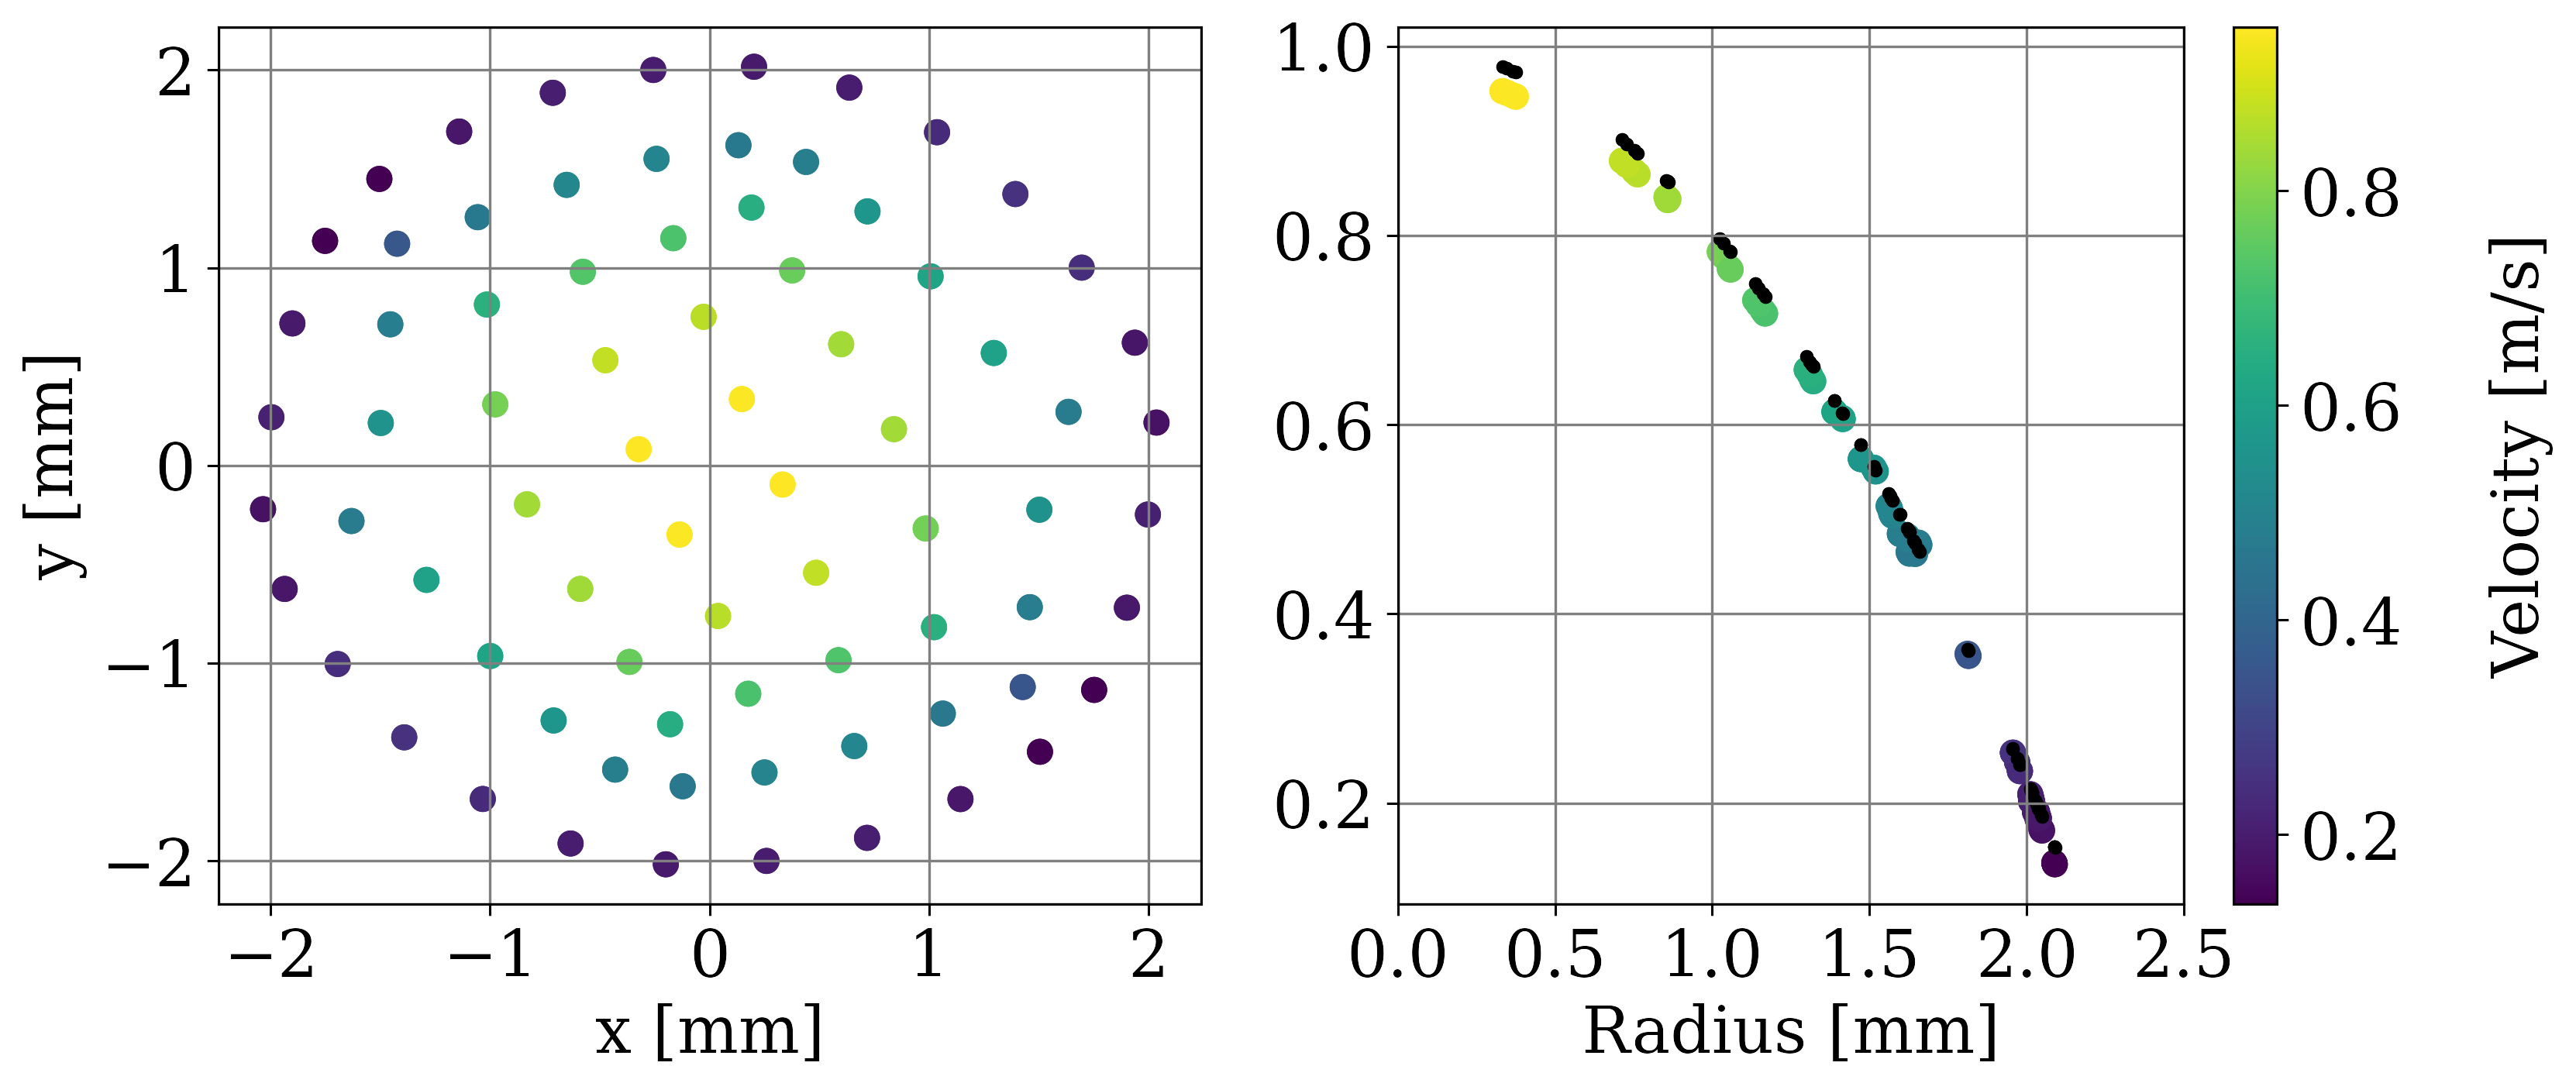
\includegraphics[width=\textwidth]{figures/code_verification/poiseuille/U_scatter_radial_z5mm_M0.png}
    \caption{Coarse Mesh}
    \label{fig:sub1}
  \end{subfigure}
  \hfill
  \begin{subfigure}[b]{0.5\textwidth}
    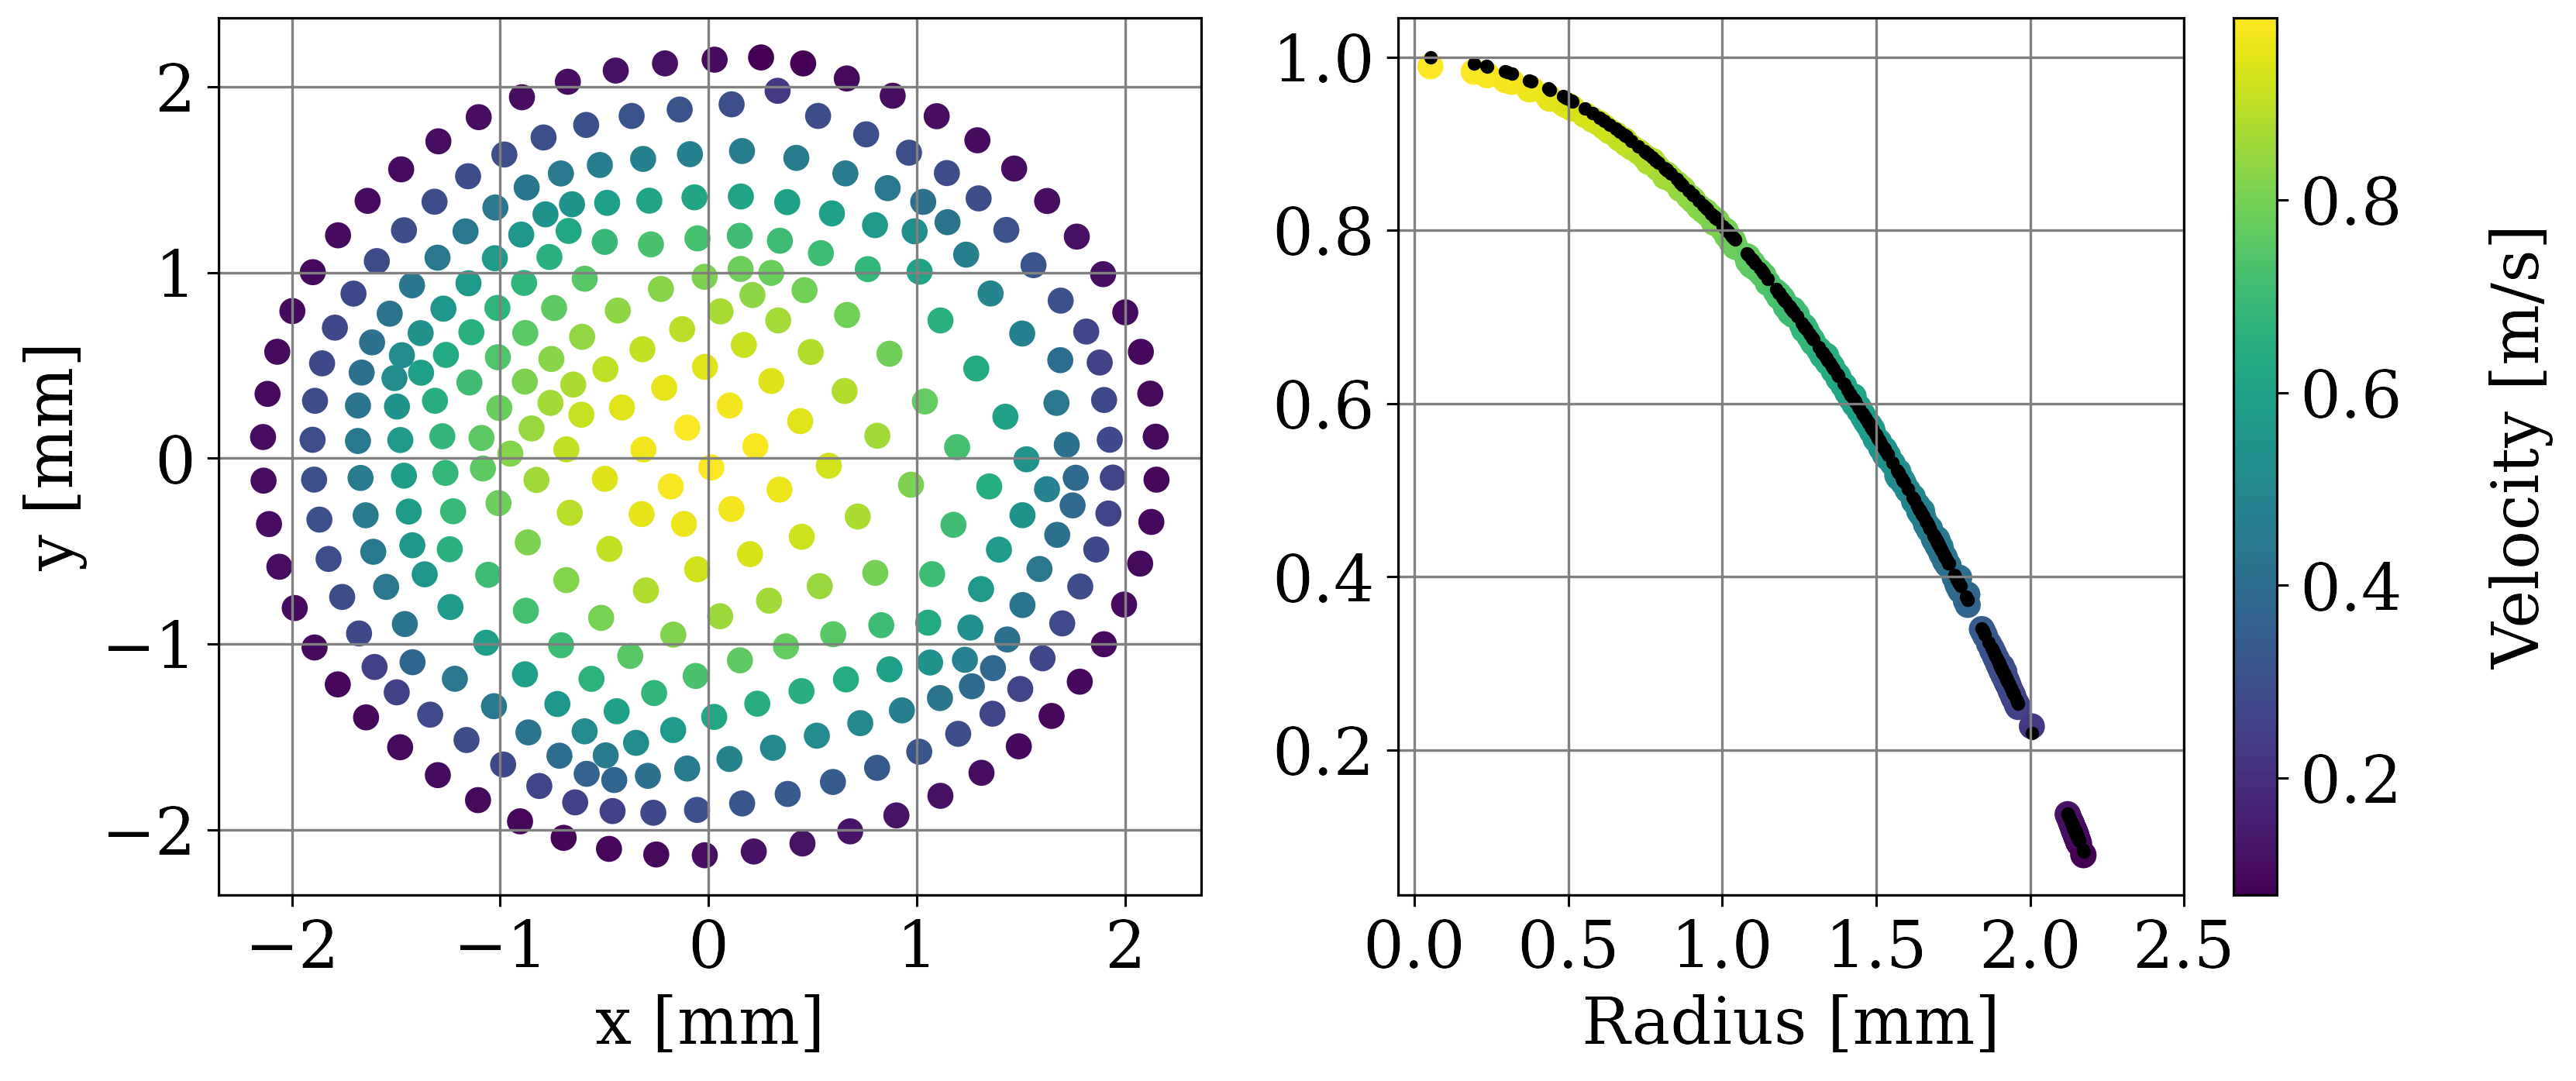
\includegraphics[width=\textwidth]{figures/code_verification/poiseuille/U_scatter_radial_z5mm_M1.png}
    \caption{Medium Mesh}
    \label{fig:sub2}
  \end{subfigure}
  \hfill
  \begin{subfigure}[b]{0.5\textwidth}
    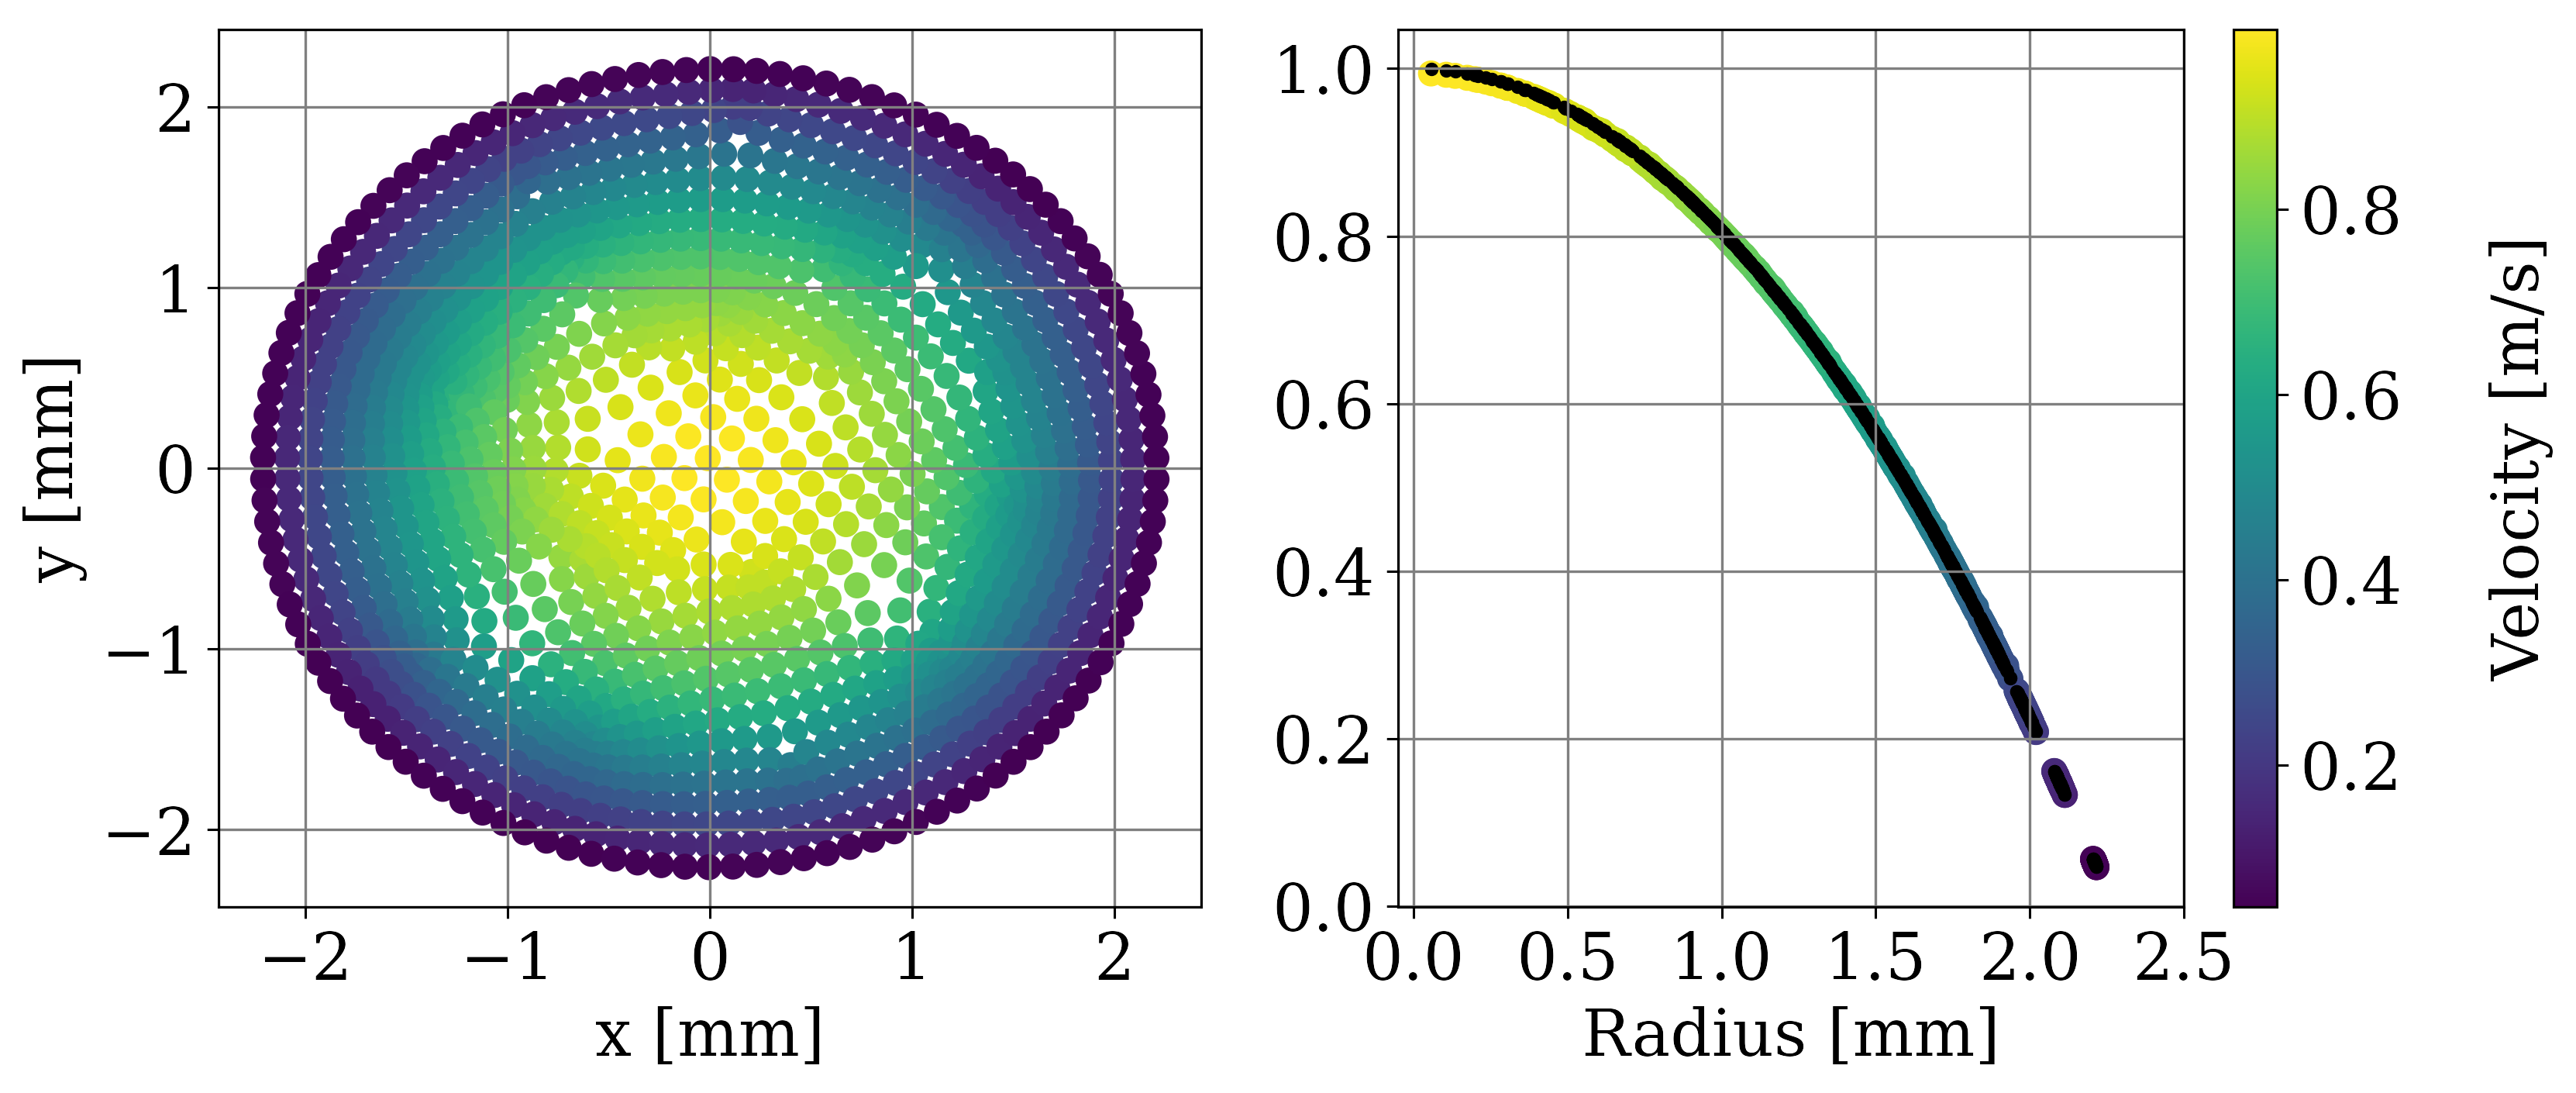
\includegraphics[width=\textwidth]{figures/code_verification/poiseuille/U_scatter_radial_z5mm_M2.png}
    \caption{Fine Mesh}
    \label{fig:sub3}
  \end{subfigure}
  \caption{Simulated hydrodynamic model axial velocity by radial position at $QoI_{\text{hydro}}$, overlaid with the analytical Hagen-Poiseuille solution (black points).}
  \label{fig:scatterVelocity}
\end{figure}

The normalized $L_2$ error was evaluated for each mesh and plotted against representative cell length (Figure~\ref{fig:errorVsLength}). The error decreases consistently with mesh refinement, yielding an observed order of convergence of $p = 1.95$. This behavior is consistent with the expected second-order accuracy of the spatial discretization scheme. These results confirm that the numerical solver accurately represents the analytical velocity field.

\begin{figure}[htbp!]
    \centering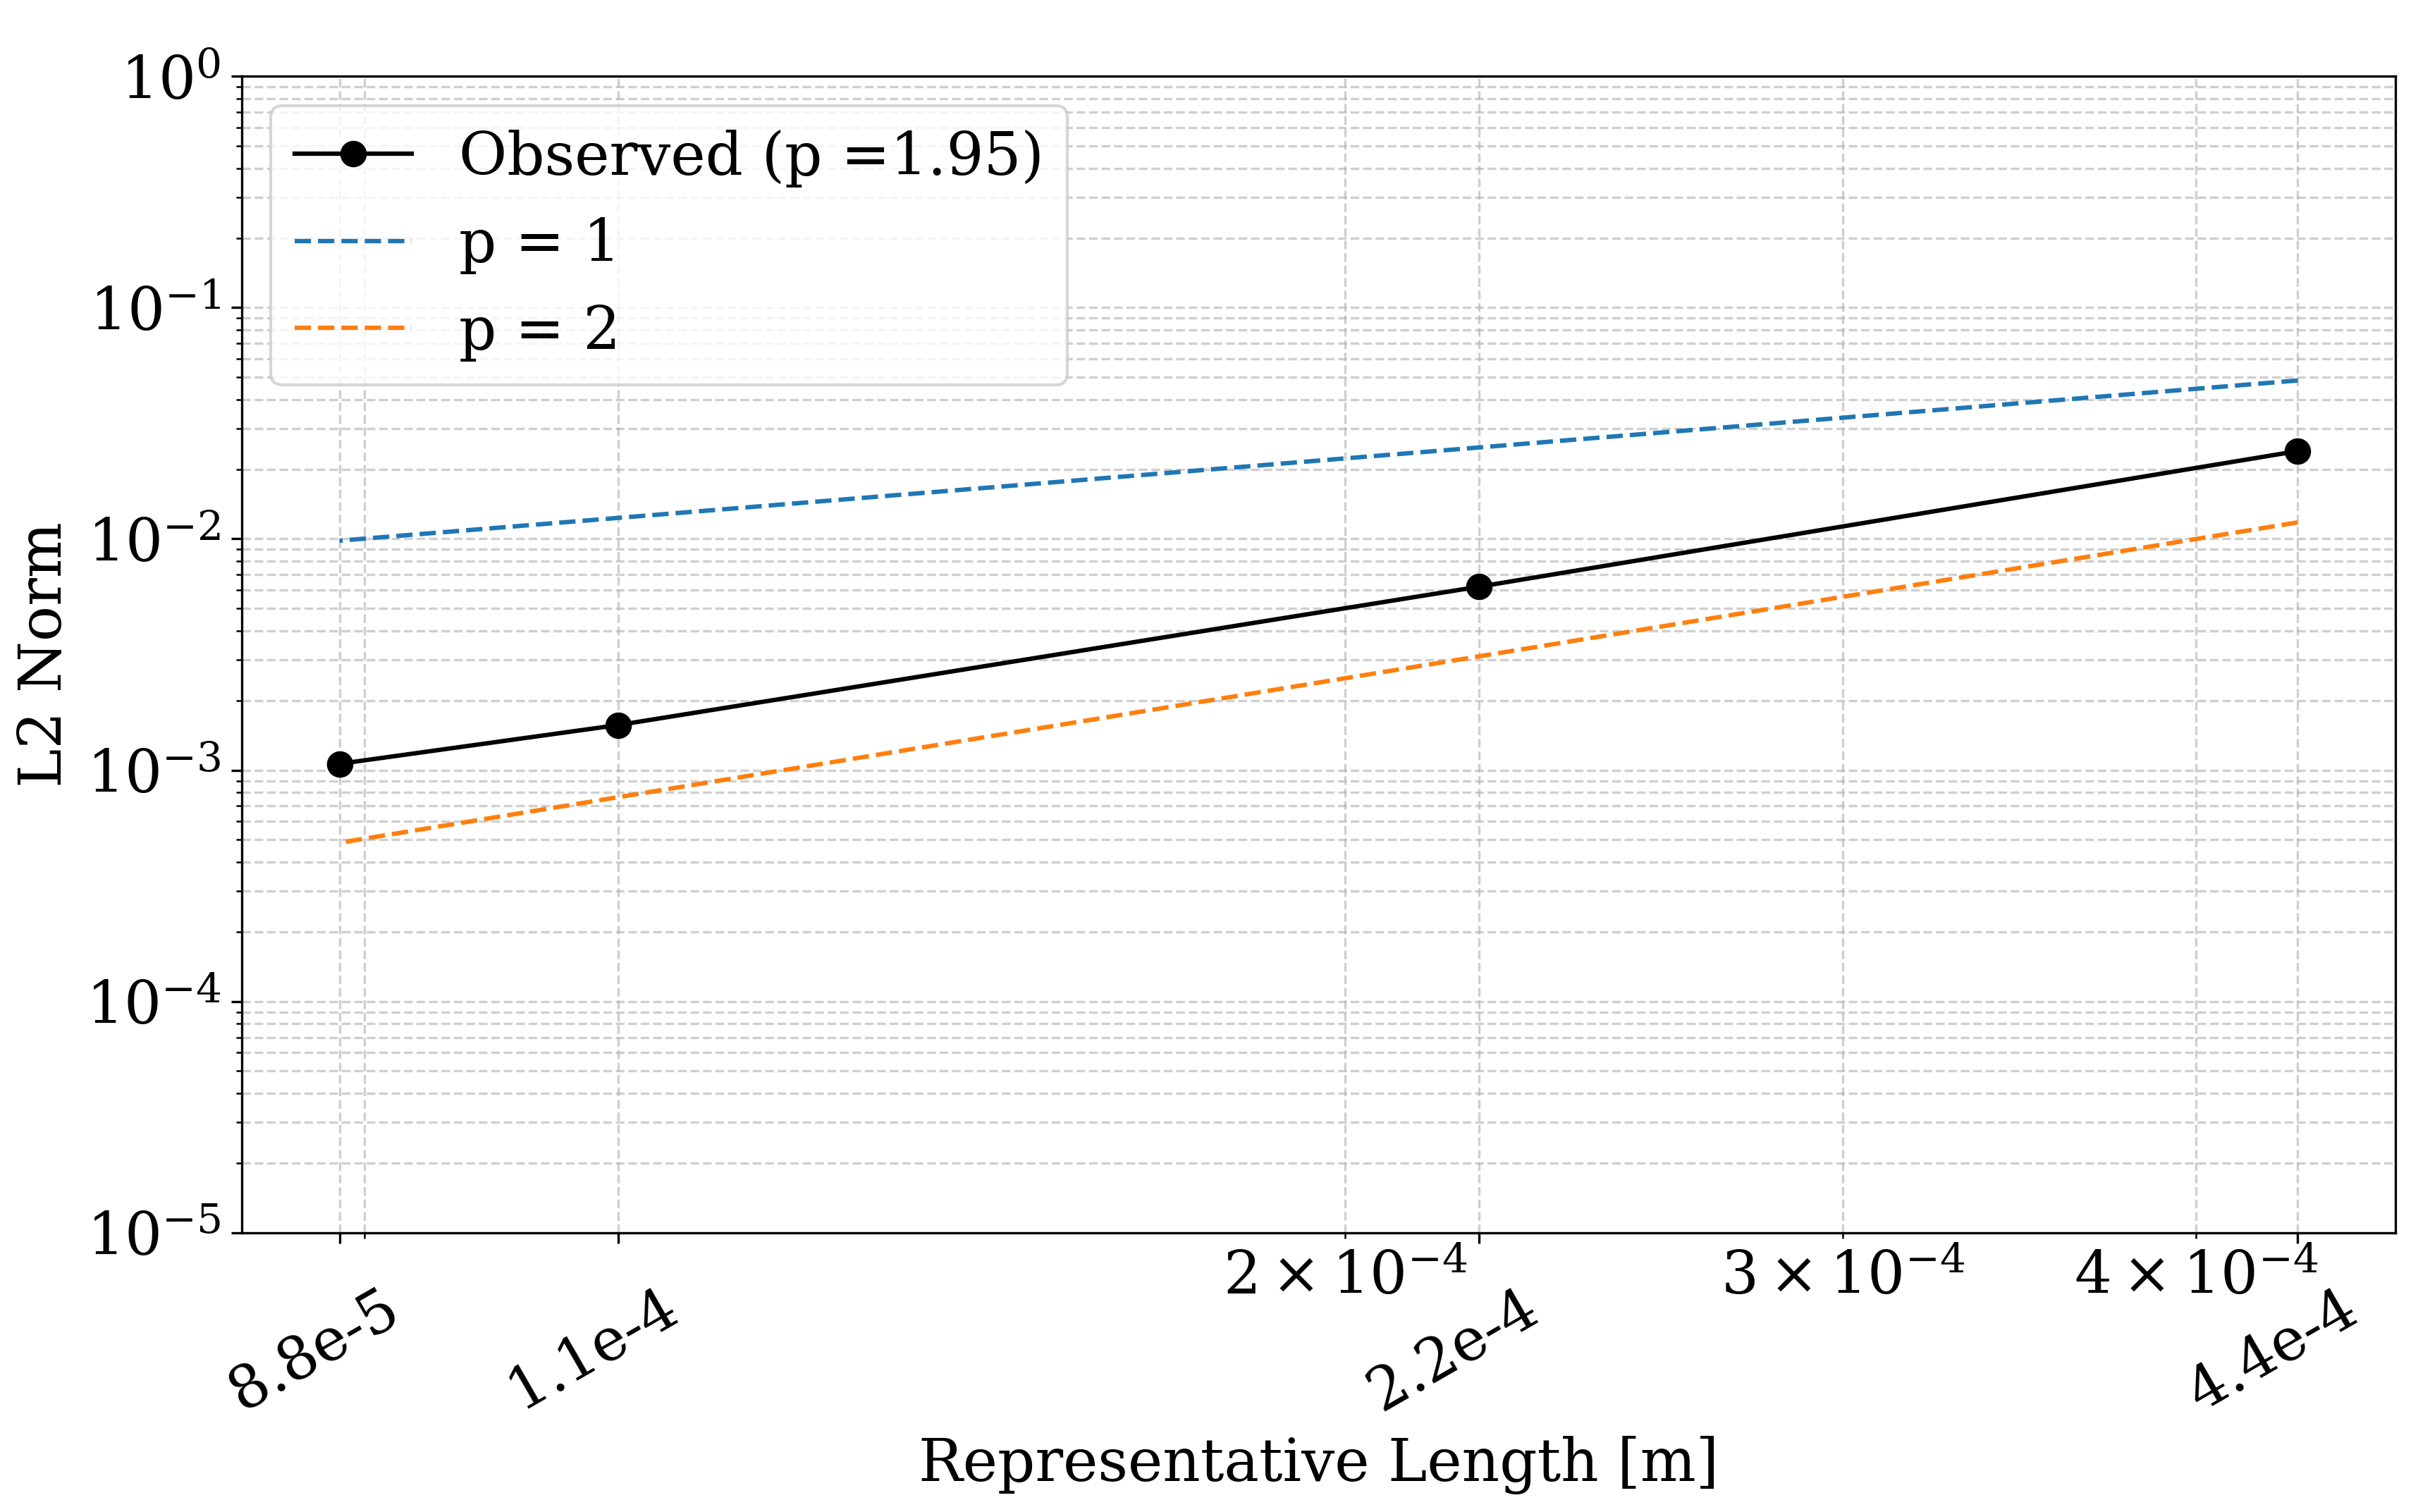
\includegraphics[width=0.95 \linewidth]{figures/code_verification/poiseuille/U_L2Norm_Observed_p.png} 
        \caption{Hydrodynamic model velocity $L_2$ error by representative cell length.}
        \label{fig:errorVsLength}
\end{figure}

\subsubsection{Radial Conduction Model}
To verify the implementation of the solid energy equation, a steady-state conduction-dominated configuration was constructed with the \texttt{chtMultiRegionFoam} solver. The problem was formulated such that the governing equations reduce to a one-dimensional radial conduction with uniform volumetric heat generation in the solid, enabling direct comparison with the analytical solution. Spatial convergence was assessed using three progressively refined meshes with representative cell sizes of 0.14~mm, 0.071~mm, and 0.035~mm. Temperature was evaluated at a cross-sectional plane sufficiently far from inlet and outlet effects to ensure a fully developed radial profile, presented in Figure~\ref{fig:scatterTemperature}.

% #Extra info: 
% Three refined meshes were used a coarse mesh with 18,000 nodes and a representative cell length of 0.14mm, a medium mesh with 144,000 nodes and a representative length of 0.071 mm, and a fine mesh with 1,152,000 nodes and a representative length of 0.035 mm. Axial Temperature are sampled across $z$ = 67.5 mm, a location far enough from the inlet and outlet. 

\begin{figure}[htbp]
  \centering
  \begin{subfigure}[b]{0.5\textwidth}
    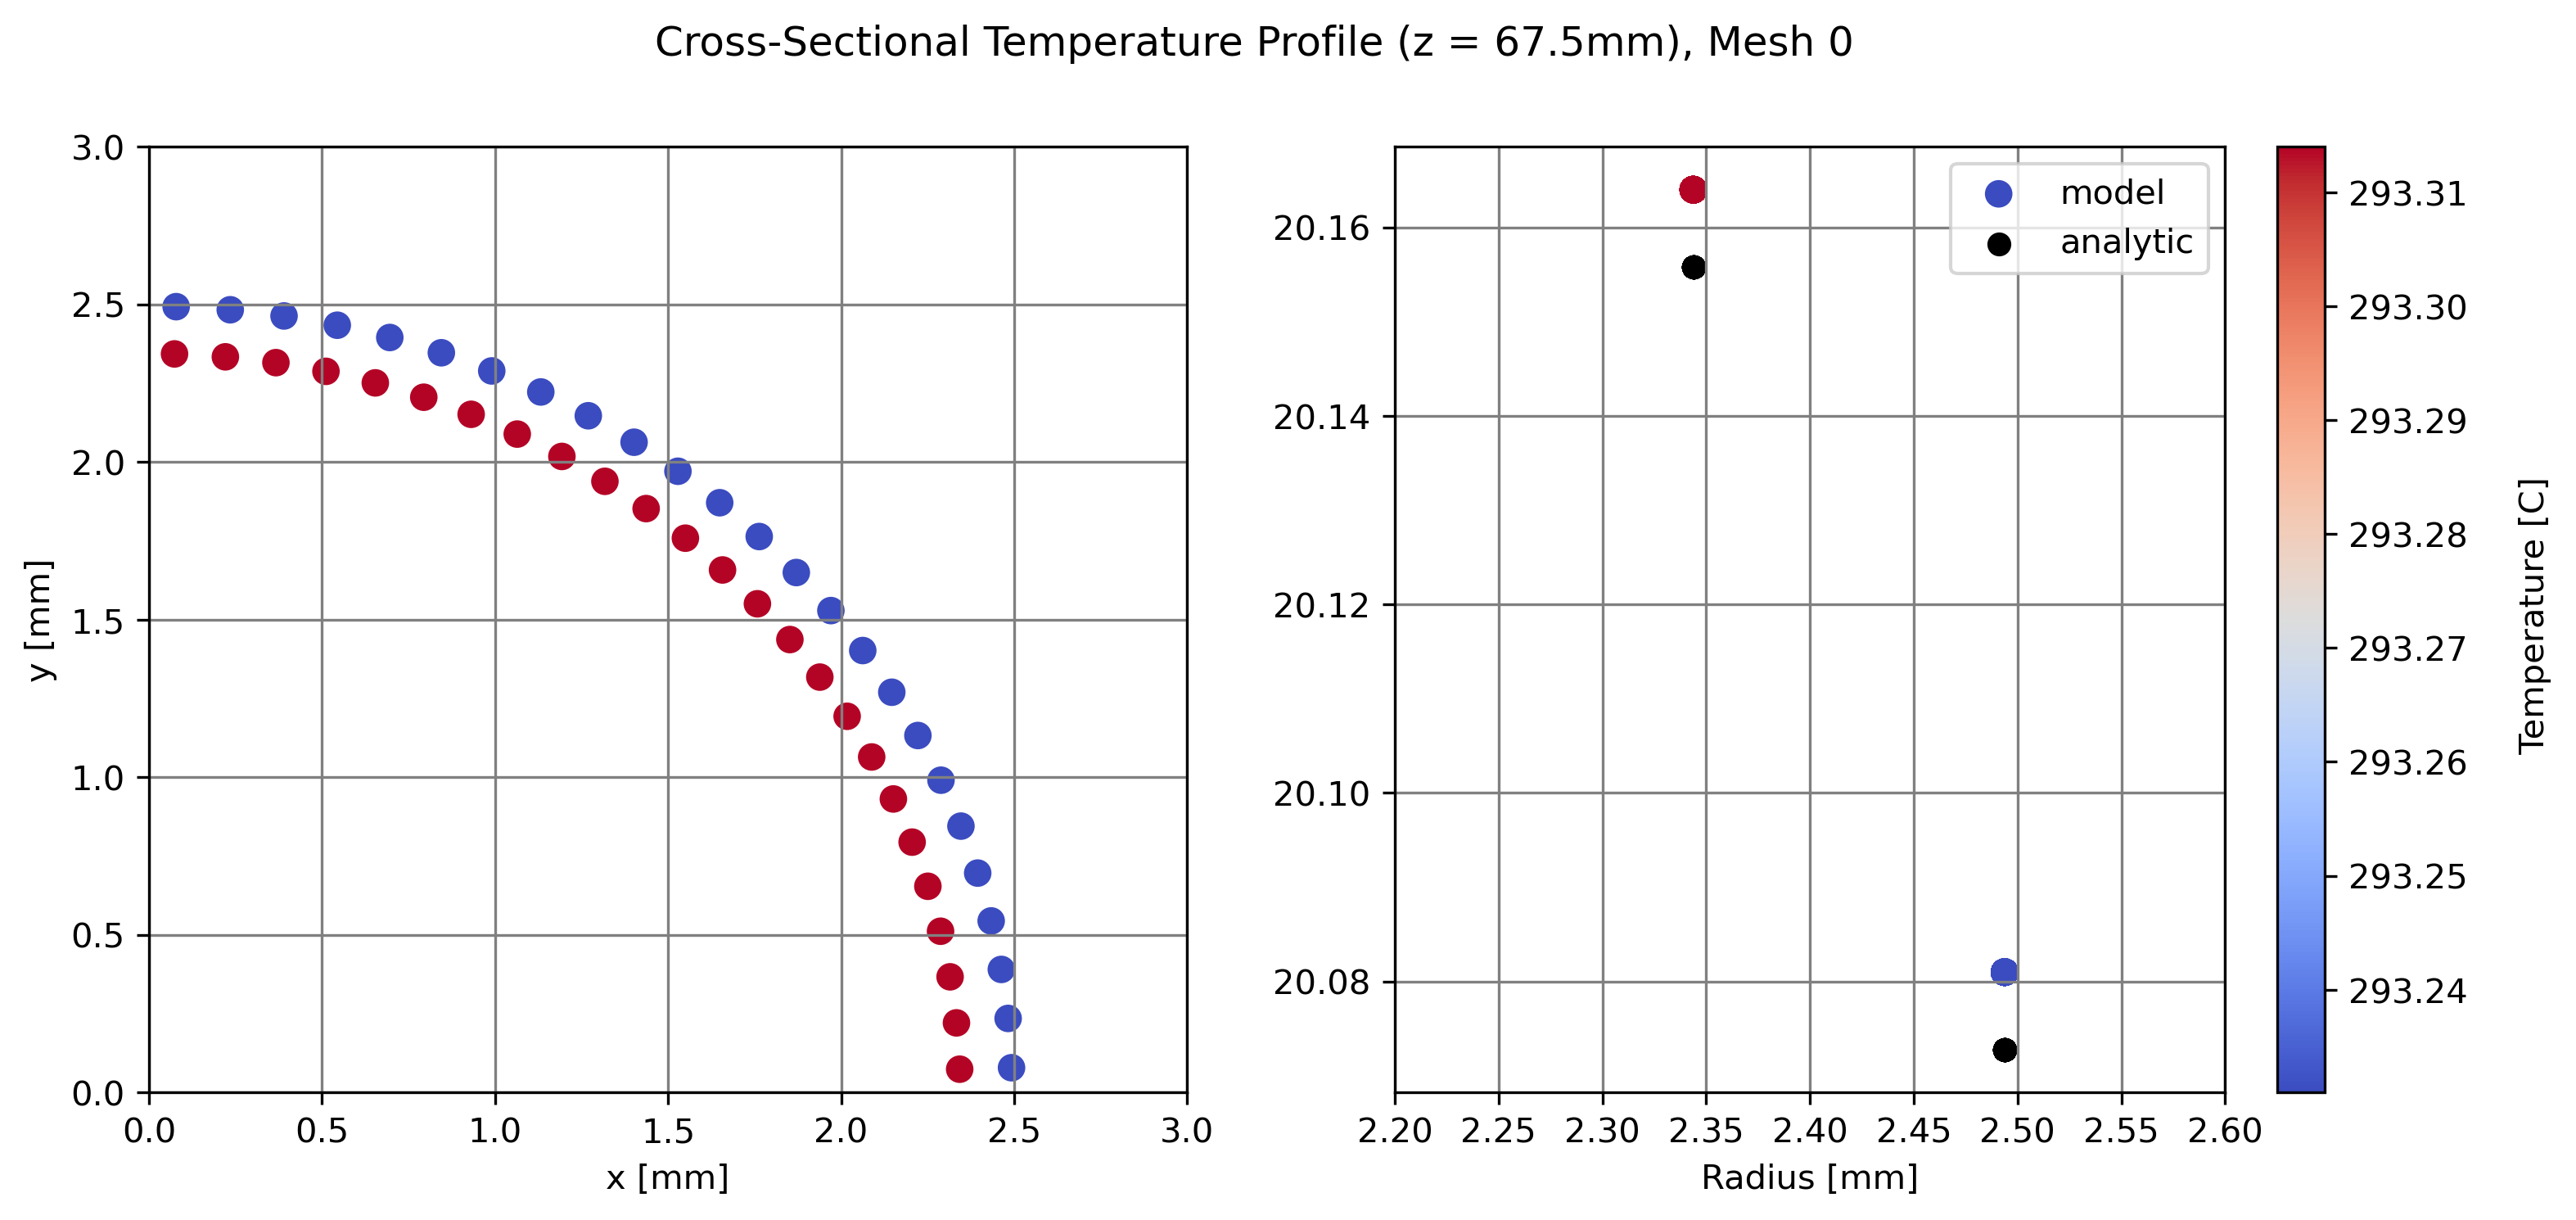
\includegraphics[width=\textwidth]{figures/heatsource/T_scatter_radial_z67.5mm_M0.png}
    \caption{Coarse mesh. }
    \label{fig:sub1T}
  \end{subfigure}
  \hfill
  \begin{subfigure}[b]{0.5\textwidth}
    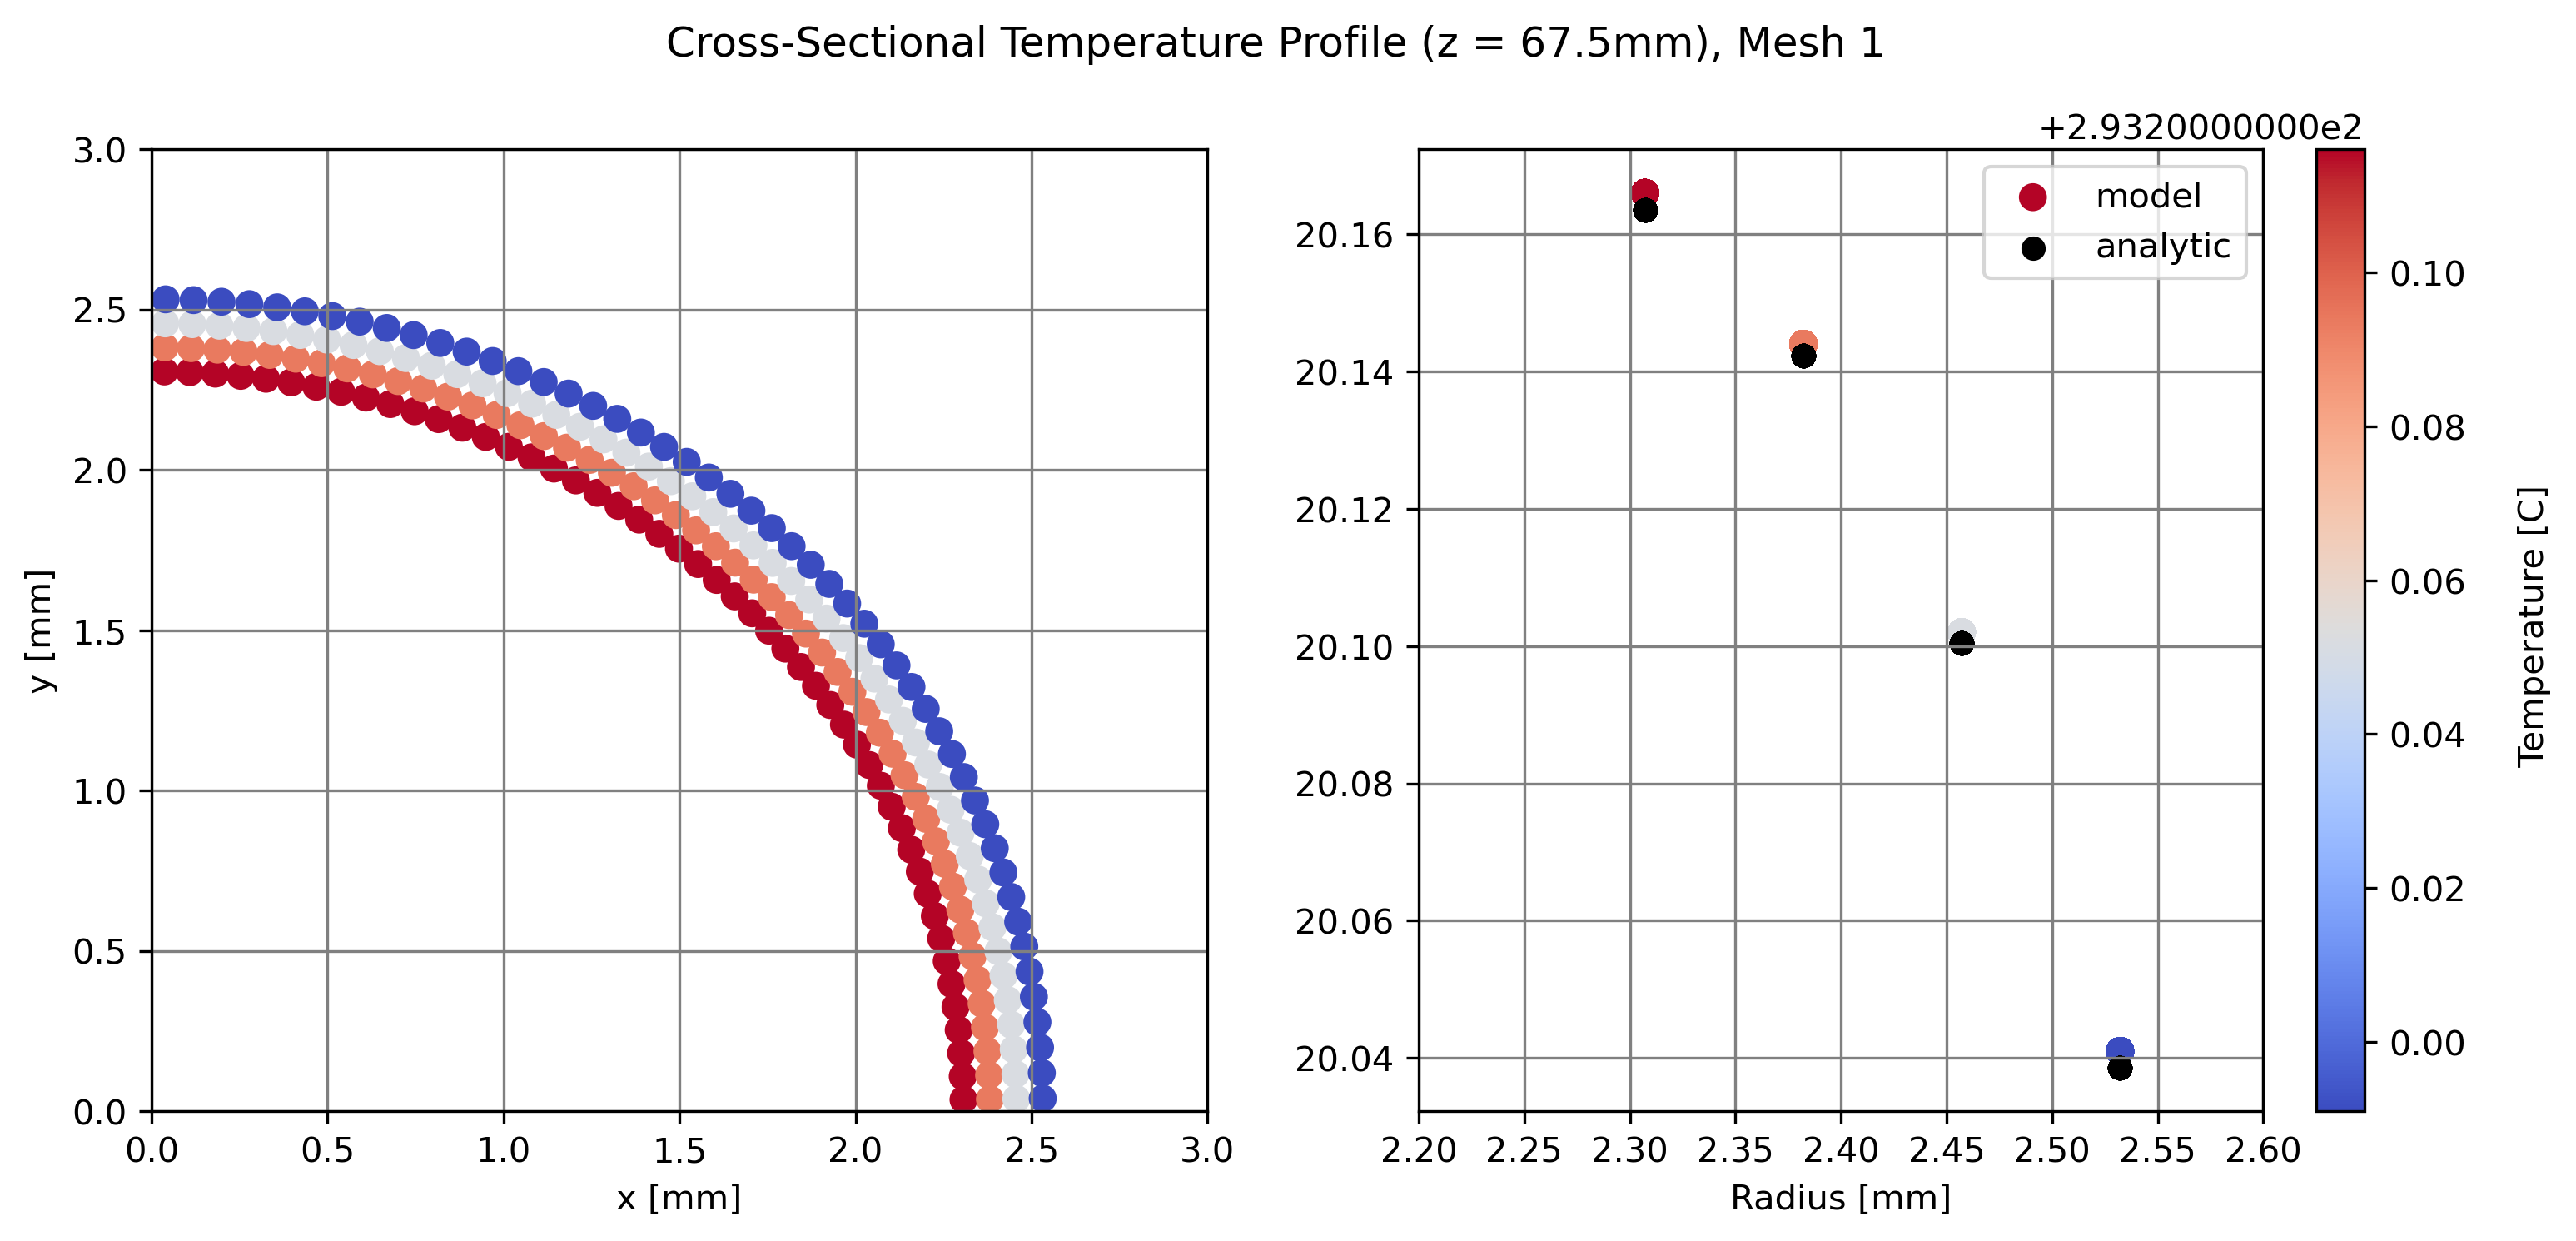
\includegraphics[width=\textwidth]{figures/heatsource/T_scatter_radial_z67.5mm_M1.png}
    \caption{Medium mesh.}
    \label{fig:sub2T}
  \end{subfigure}
  \hfill
  \begin{subfigure}[b]{0.5\textwidth}
    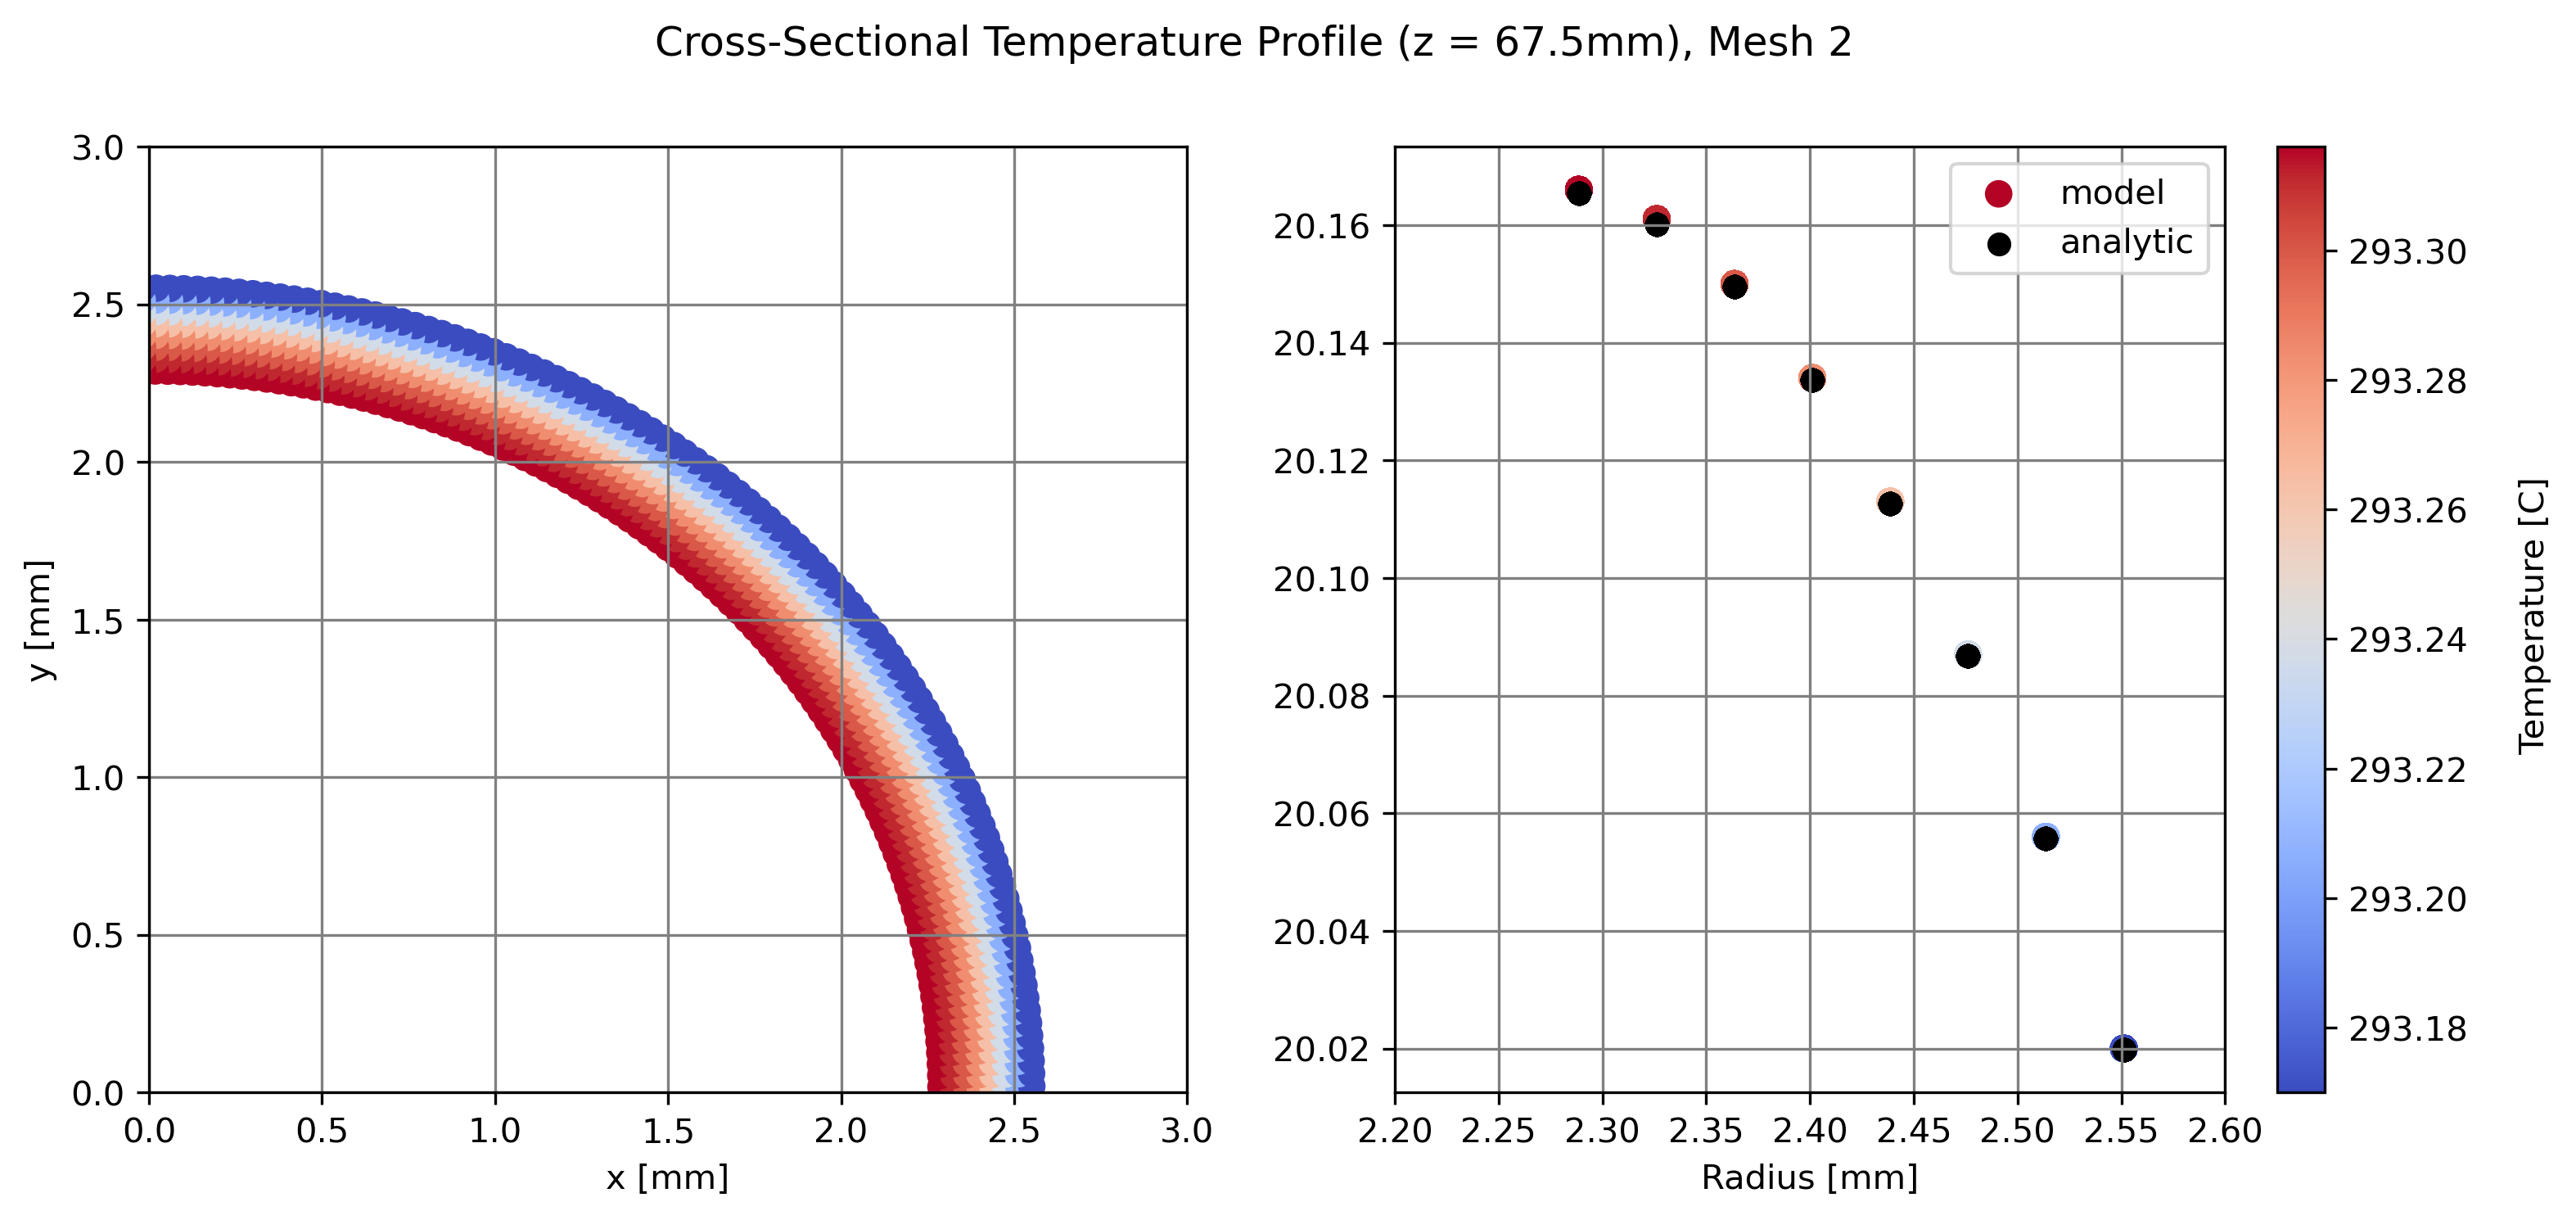
\includegraphics[width=\textwidth]{figures/heatsource/T_scatter_radial_z67.5mm_M2.png}
    \caption{Fine mesh.}
    \label{fig:sub3T}
  \end{subfigure}
  \caption{Radial conduction model simulated temperature by radial position at $QoI_{\text{cond}}$, overlaid with the analytical solution (black points).}
  \label{fig:scatterTemperature}
\end{figure}

Figure~\ref{fig:scatterTemperature} shows that the numerical temperature field converges toward the analytical solution as mesh resolution increases. The coarse mesh exhibits noticeable deviation from the analytical profile, while refinement reduces this discrepancy and the fine mesh achieves near pointwise agreement across the radius. The normalized $L_2$ error was evaluated for each mesh and plotted against representative cell length (Figure~\ref{fig:l2normTempInterface}). The error decreases consistently with mesh refinement, producing an observed order of convergence of $p = 2.08$, which is consistent with the expected second-order spatial accuracy of the discretization scheme. The error magnitude decreases from $\mathcal{O}(10^{-4})$ to $\mathcal{O}(10^{-6})$, indicating strong agreement with the analytical solution. These results confirm that the numerical implementation of the solid energy equation is correct and exhibits the expected convergence behavior under mesh refinement.

\begin{figure}[htbp!]
    \centering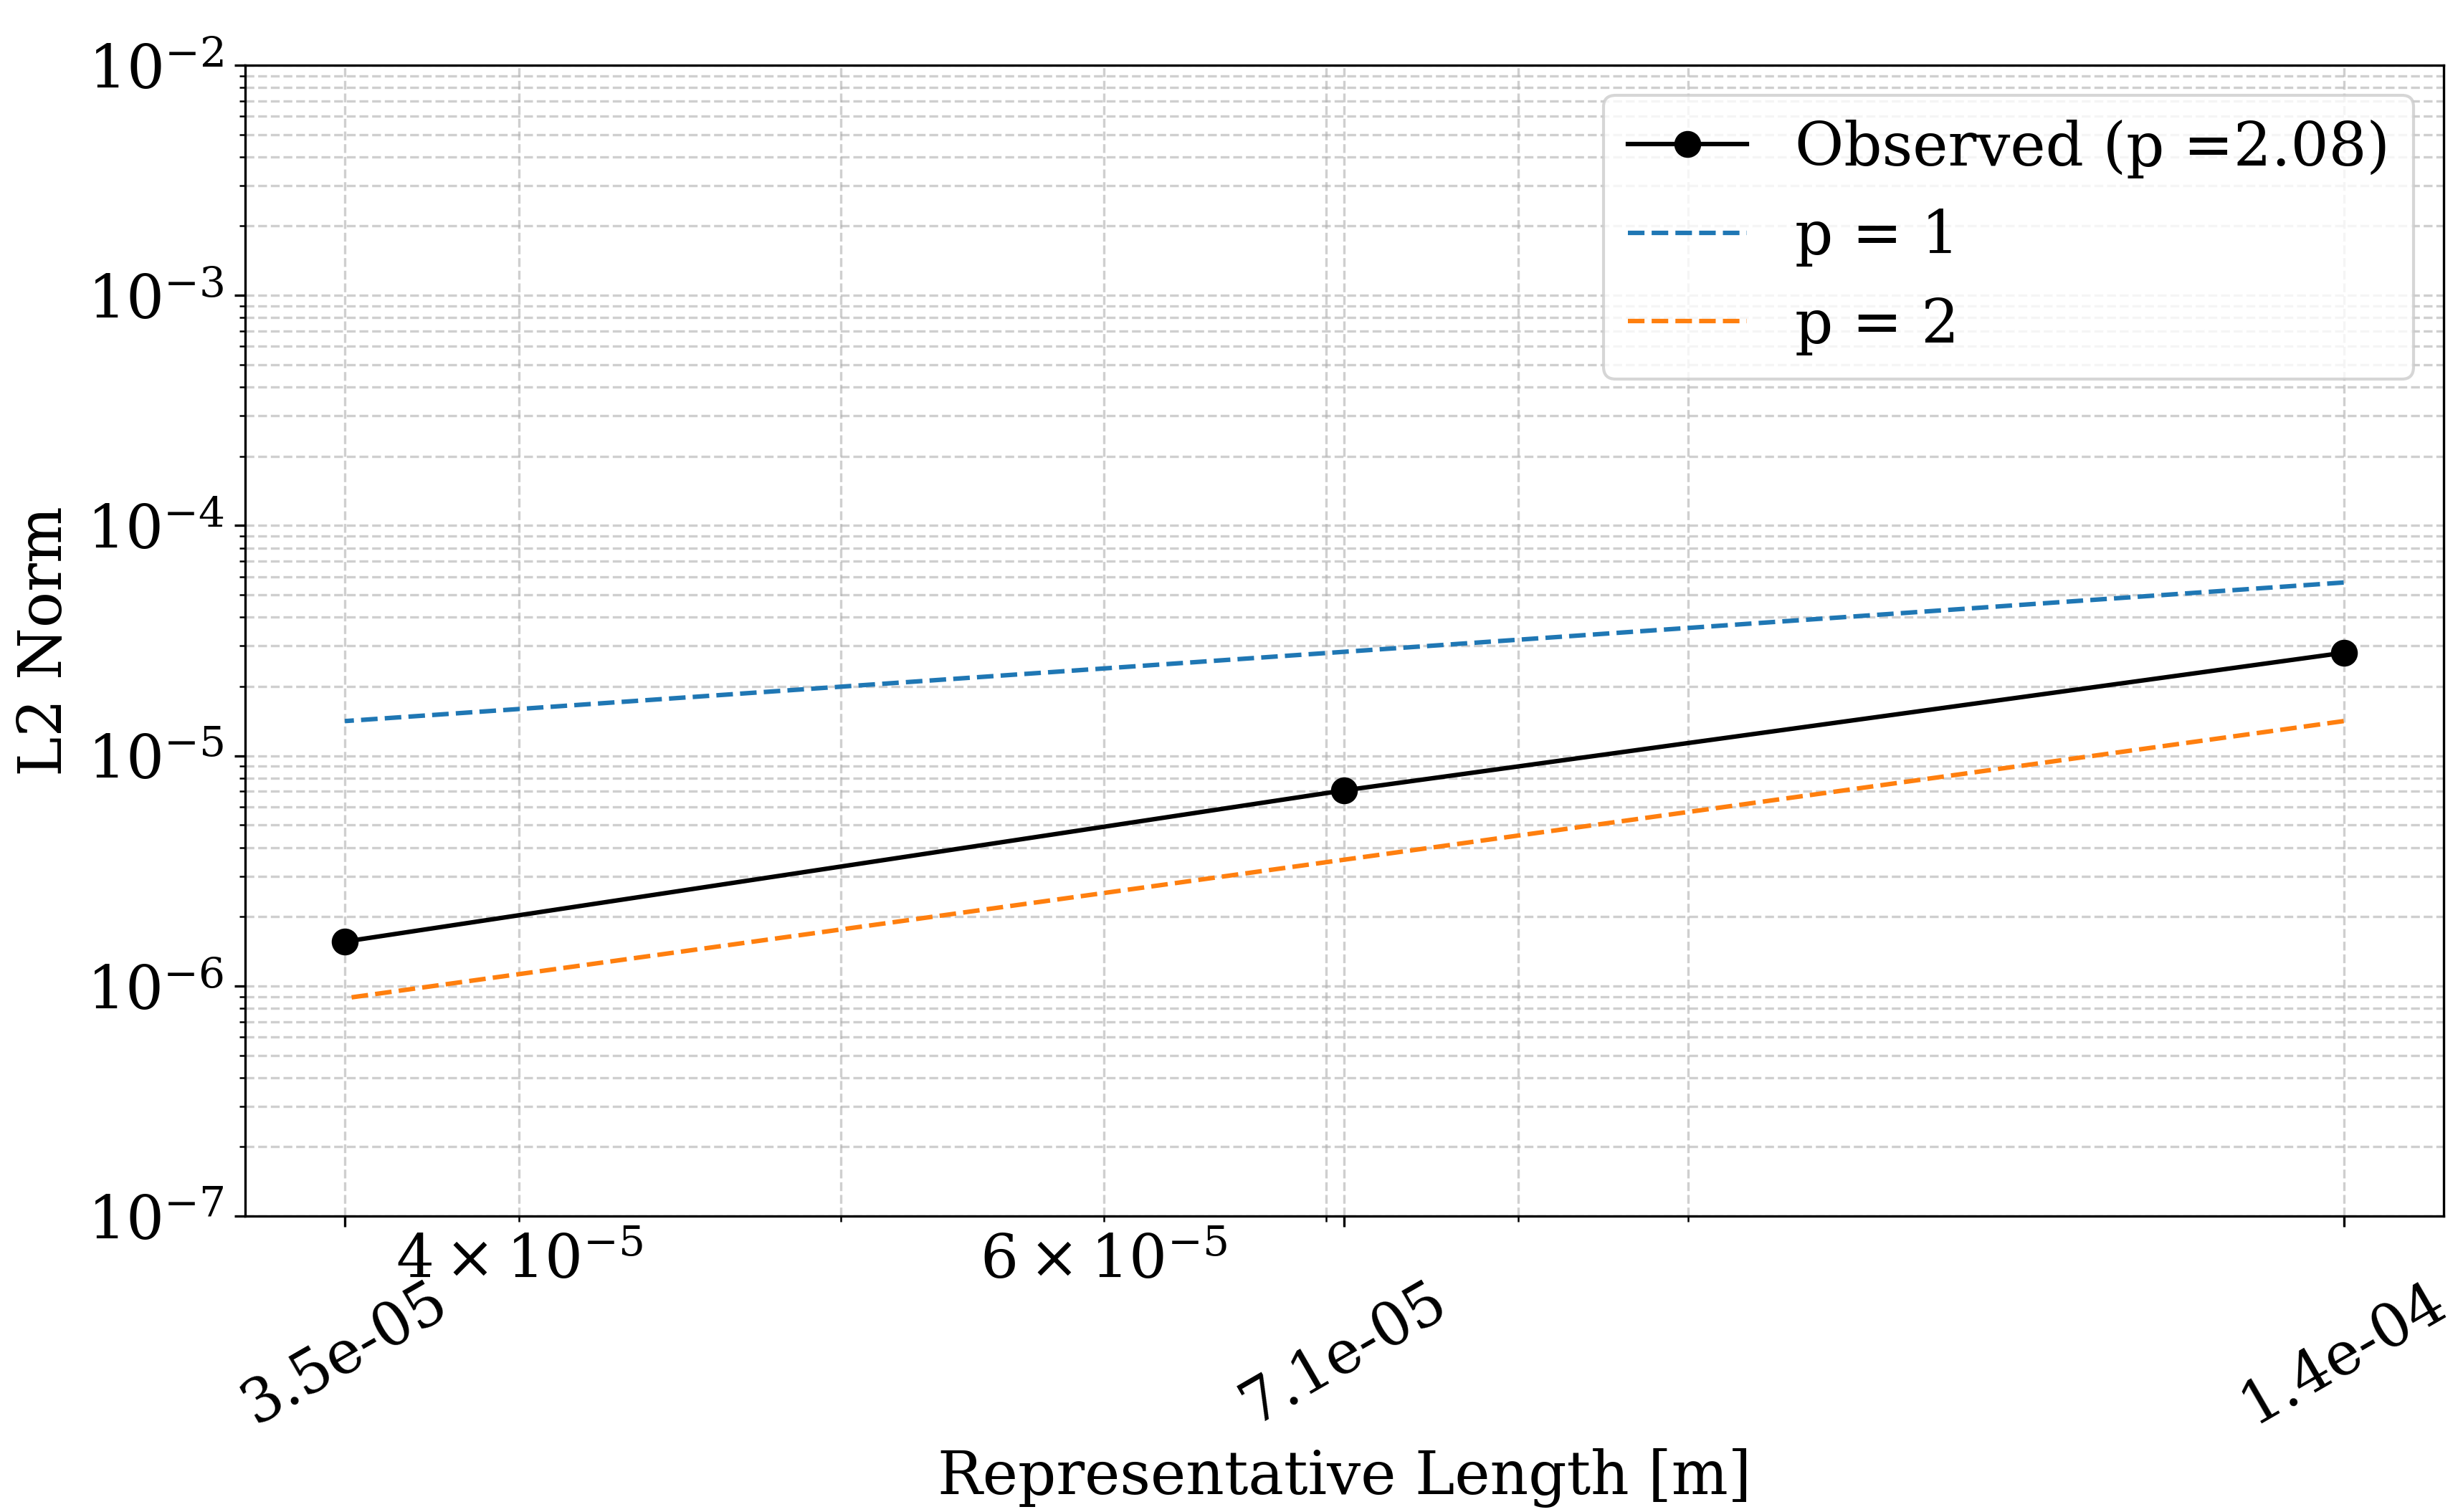
\includegraphics[width=0.95 \linewidth]{figures/heatsource/T_L2Norm_Observed_p.png} 
        \caption{Radial conduction model temperature $L_2$ error by representative cell length.}
        \label{fig:l2normTempInterface}
\end{figure}


\subsubsection{Transient Thermal Diffusion Verification}
Following isolated verification of the hydrodynamic and steady-state radial conduction models, a transient thermal diffusion case is used to bridge the isolated verification studies and the fully coupled transient conjugate heat transfer model. In order to reduce the governing energy equation to a radial diffusion problem the fluid velocity was set to zero. This isolates transient thermal transport and interface temperature transfer from the solid to the fluid region. The $L_2$ error is computed at a cross section, halfway along the heated fluid region, by comparing the simulated temperature, at each radial position, to the corresponding analytical radial temperature obtained from Eq.~\ref{eq:bessel_theta_solution} and Eq.~\ref{eq:dimensional_temperature}. Figure~\ref{fig:transientDiffusionConvergence} shows the normalized $L_2$ error as a function of representative cell size for multiple transient times. 

\begin{figure}[htbp!]
    \centering
    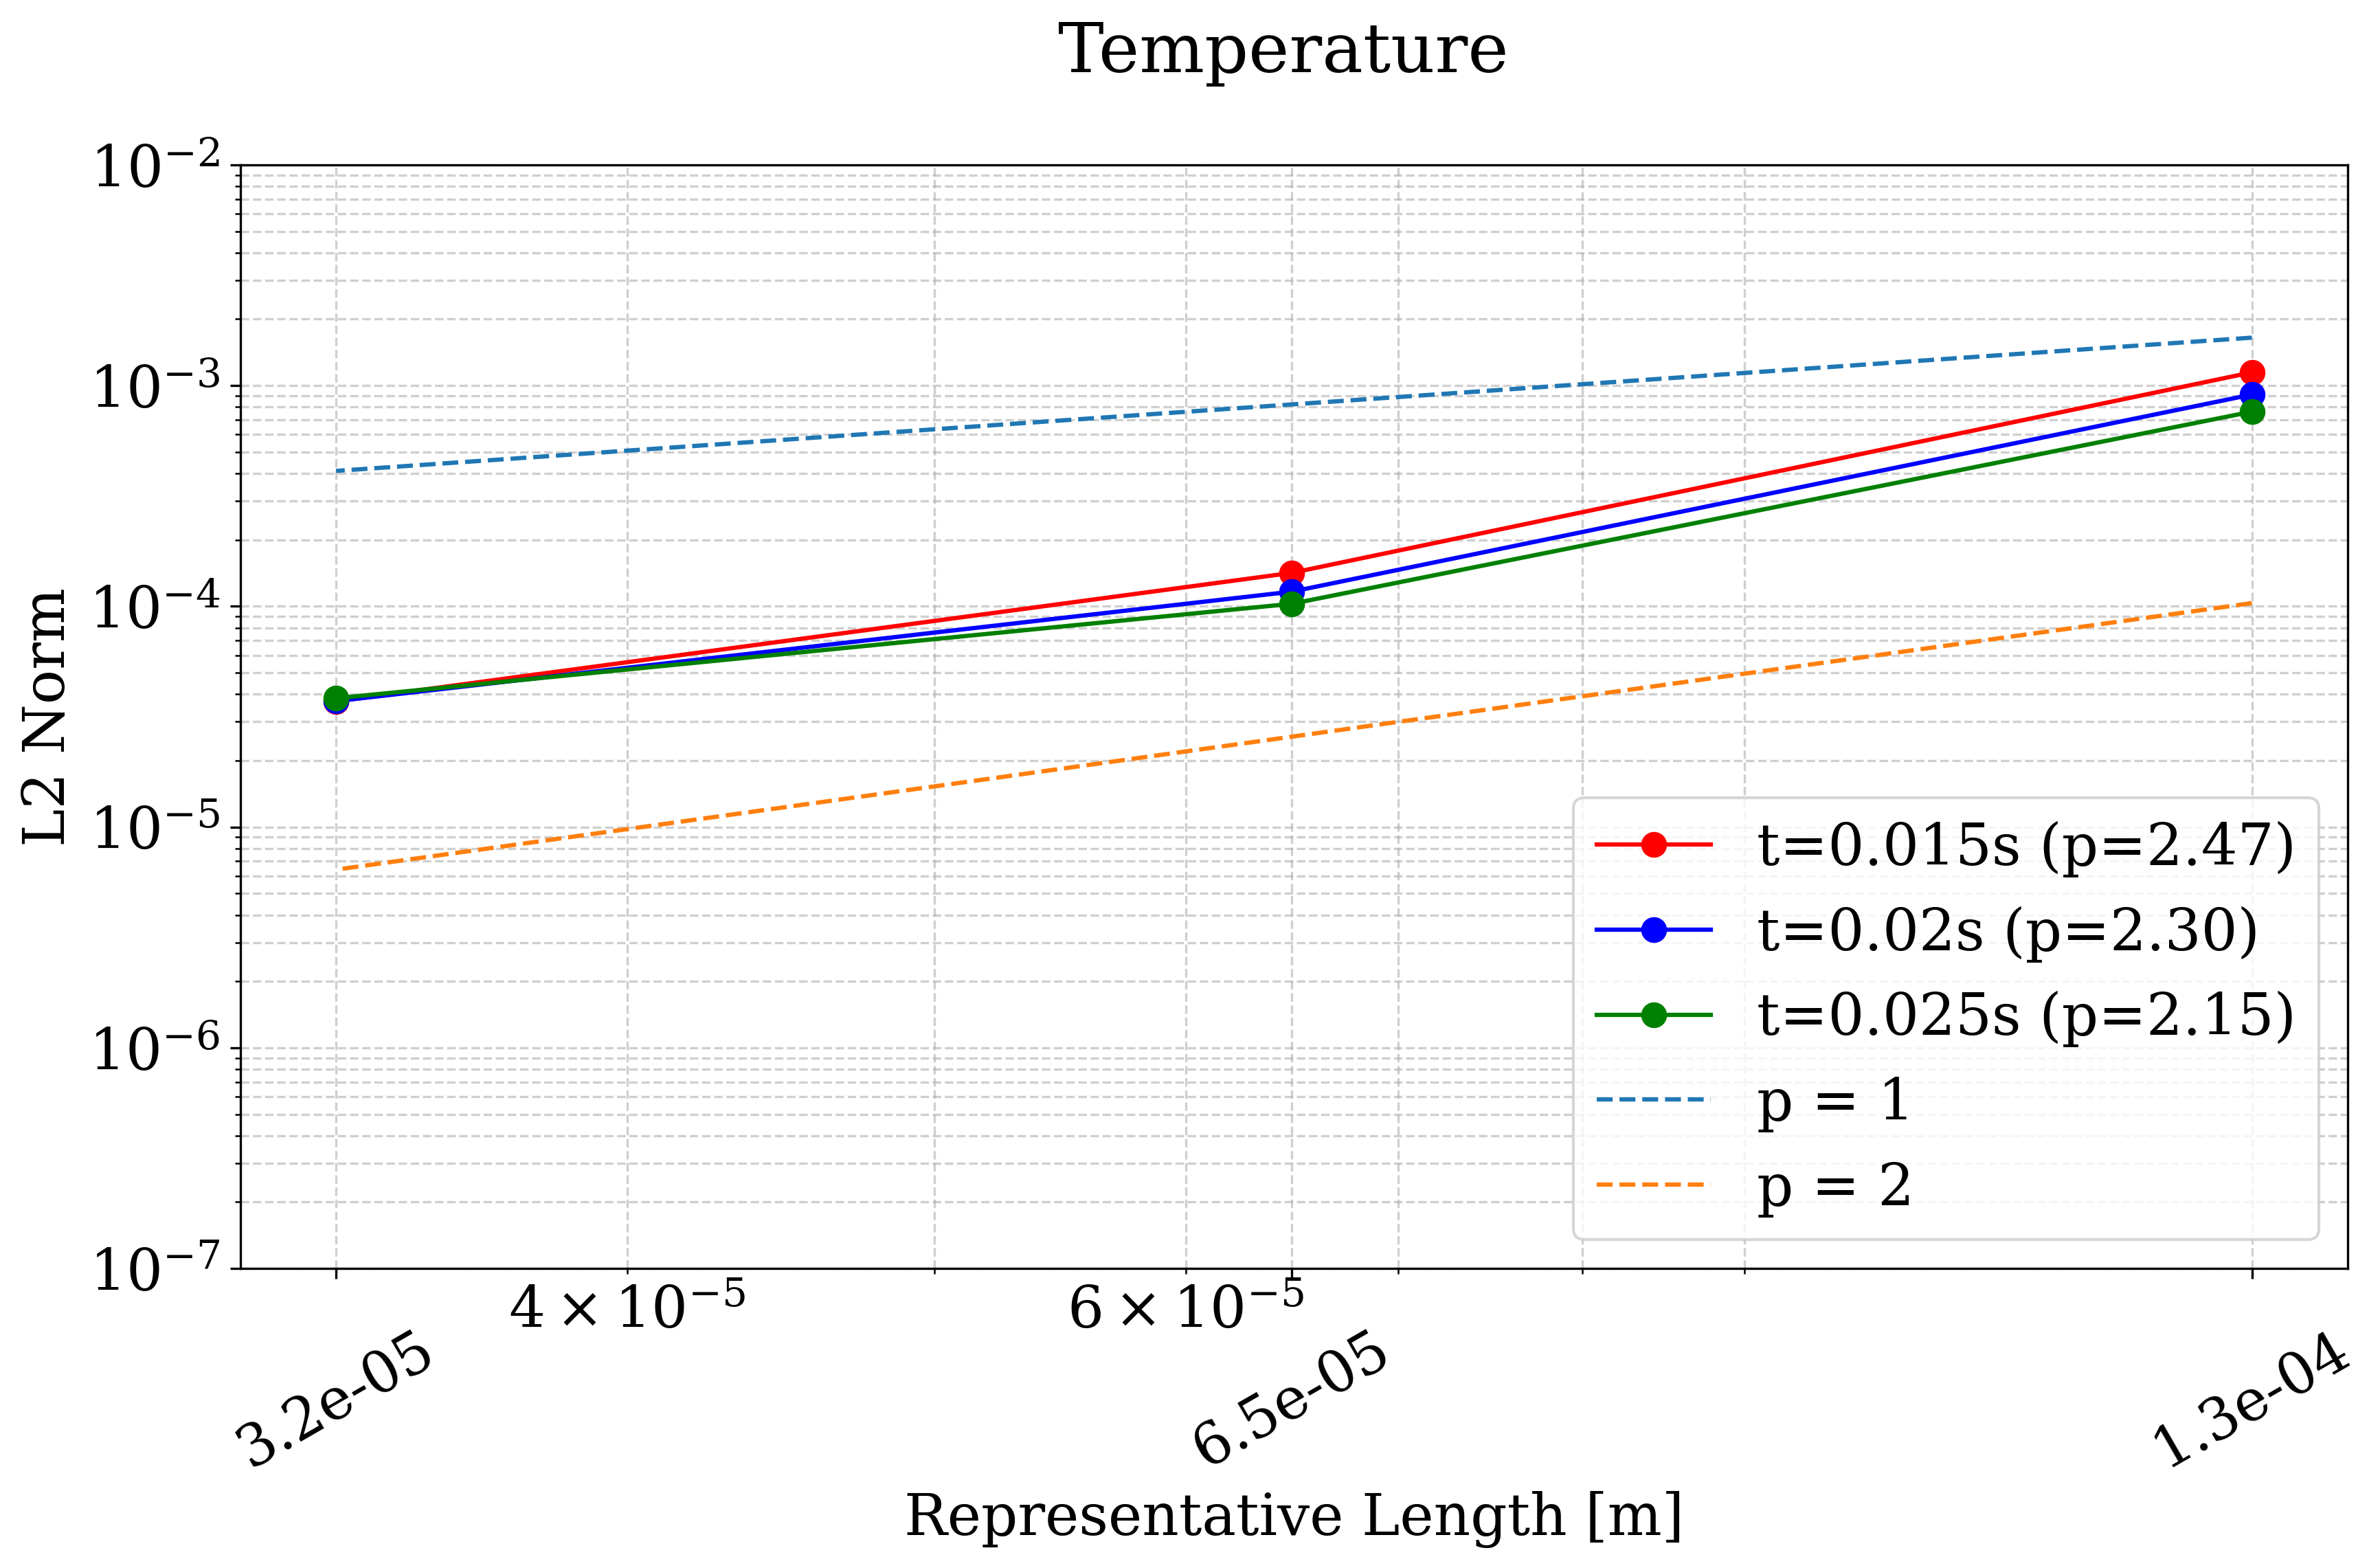
\includegraphics[width=1.0\linewidth]{figures/code_verification/interface/T_L2Norm_Observed_p_th2.png}
    \caption{Thermal diffusion model temperature $L_2$ error by representative cell length at three times.}
    \label{fig:transientDiffusionConvergence}
\end{figure}
The error decreases consistently with mesh refinement, yielding observed orders of convergence of $p=2.47$ at $t=0.015$~s, $p=2.30$ at $t=0.020$~s, and $p=2.15$ at $t=0.025$~s, showing near second-order spatial accuracy. Larger errors occur at earlier times due to stronger thermal gradients, while later times exhibit reduced error magnitudes as the solution becomes increasingly diffused. These results demonstrate that the solver accurately captures transient thermal diffusion behavior and correctly transfers the imposed solid temperature response across the fluid-solid interface under transient conditions.

\subsection{Solution Verification} 
Solution verification results are presented to quantify numerical error arising from spatial and temporal discretization, as well as solver convergence. The analysis focuses on the impact of mesh resolution, time step size, and solver tolerance on the predicted temperature response. The following studies evaluate convergence behavior and discretization error for both steady-state and transient models, building the accuracy and reliability of the coupled fluid-thermal solution.

\subsubsection{Steady-State Coupled Pipe}
Following independent verification of the fluid and solid governing equations, a fully coupled conjugate heat transfer (CHT) configuration is considered to assess the combined system behavior. The discretization error is evaluated through systematic mesh refinement under steady-state conditions. Figure~\ref{fig:scatterTemp} shows the radial temperature distribution within the thermally developing region, located 14 mm downstream of the start of heating. The highest temperatures occur near the wall where heat is introduced, while lower temperatures are near the centerline due to the developing thermal boundary layer. As mesh resolution increases, the temperature field becomes smoother and more consistent.

\begin{figure}[htbp]
  \centering
  \begin{subfigure}[b]{0.5\textwidth}
    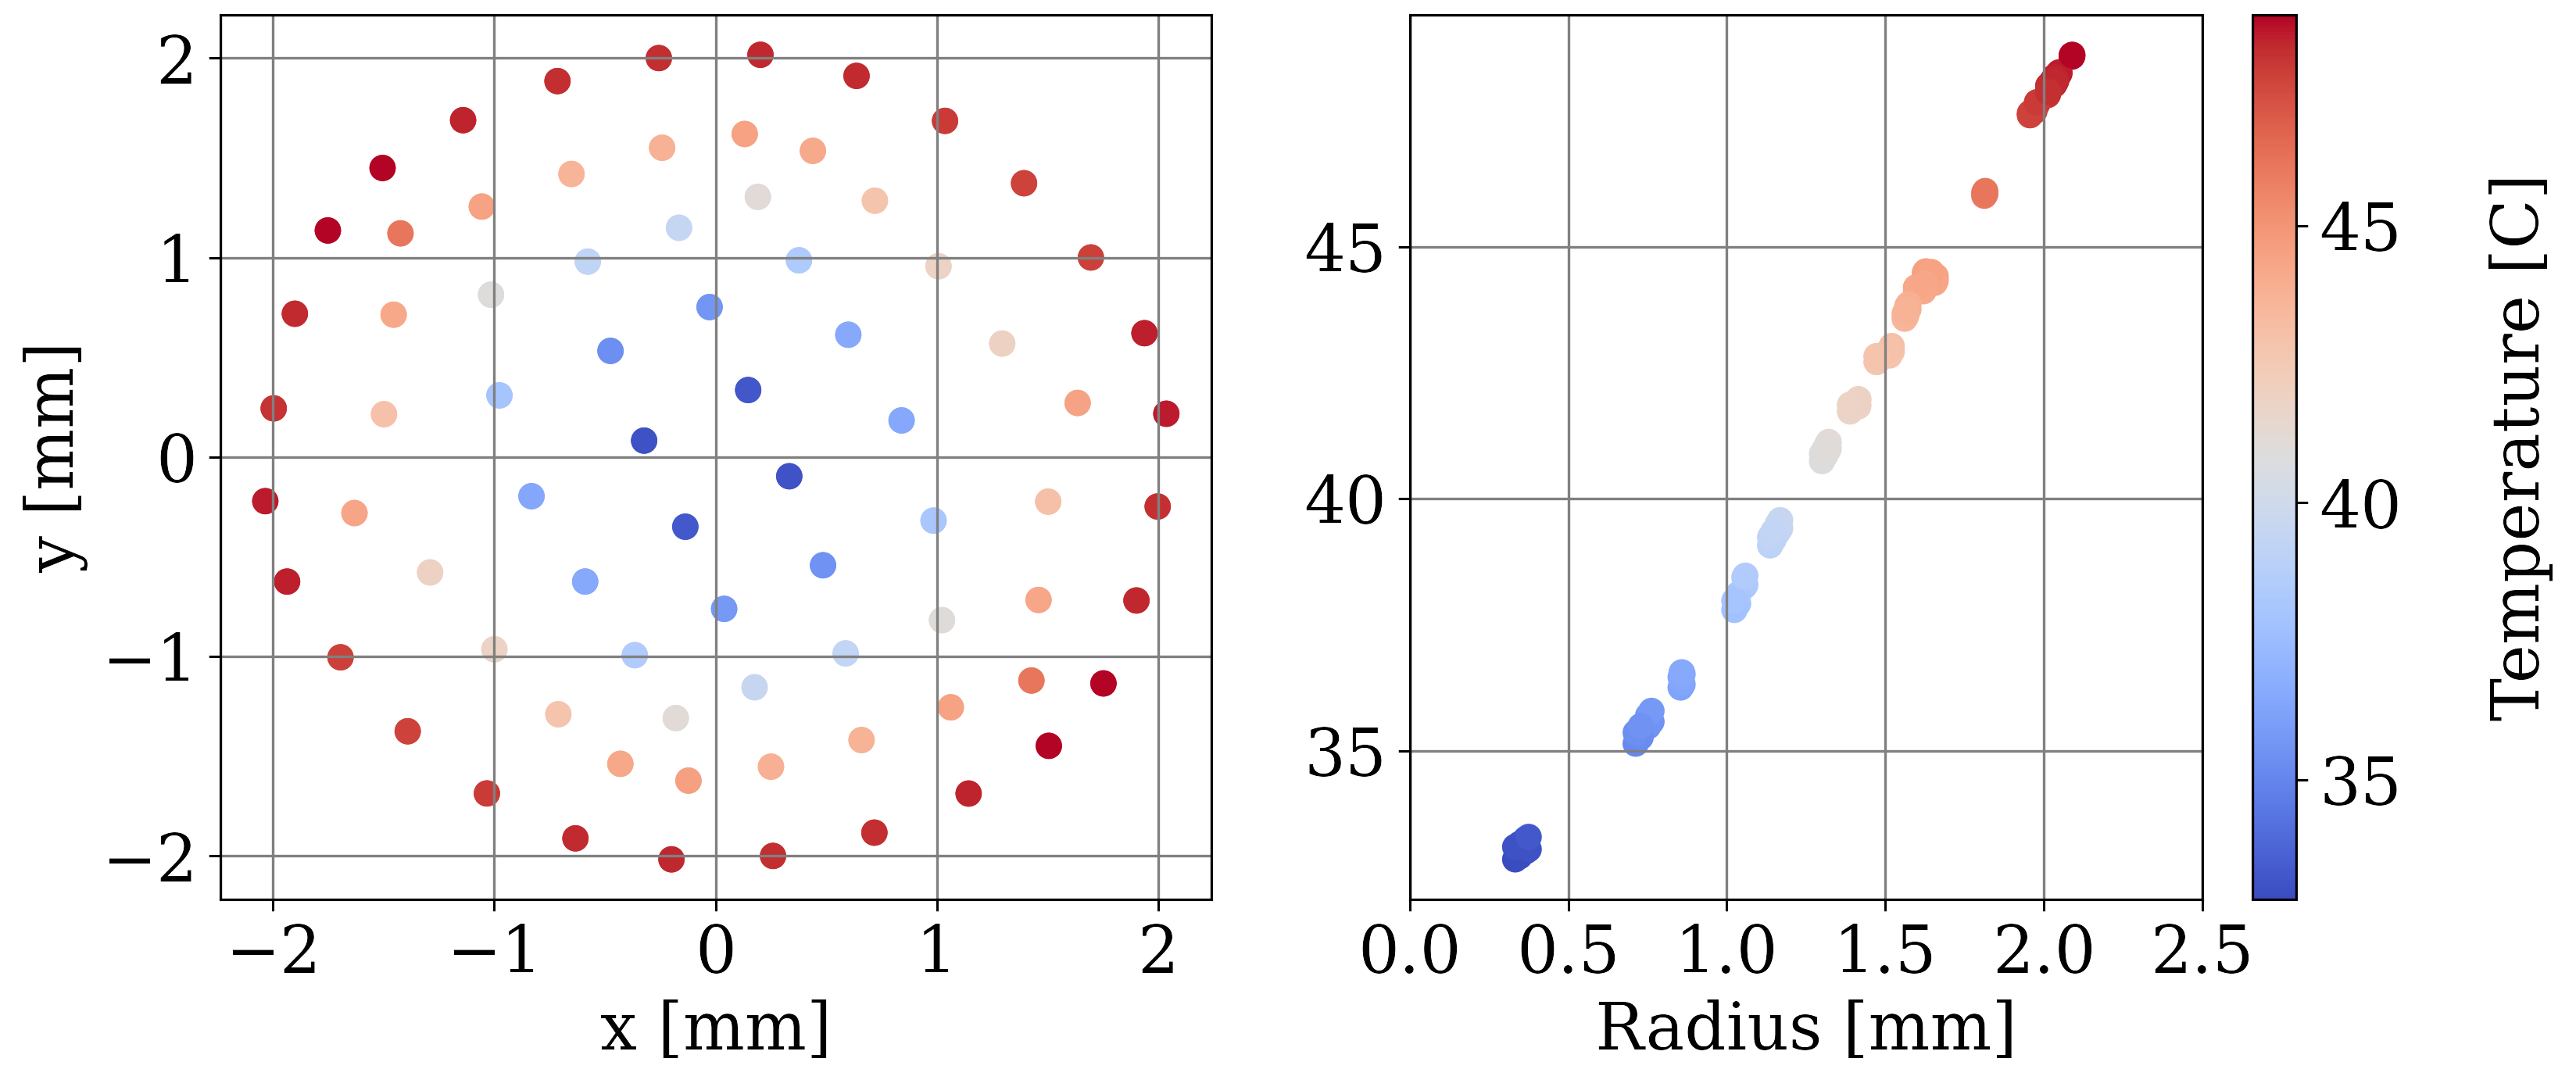
\includegraphics[width=\textwidth]{figures/code_verification/graetz/T_scatter_radial_z30mm_M0.png}
    \caption{Coarse mesh.}
    \label{fig:sub1}
  \end{subfigure}
  \hfill
  \begin{subfigure}[b]{0.5\textwidth}
    \includegraphics[width=\textwidth]{figures/code_verification/graetz/T_scatter_radial_z30mm_m1.png}
    \caption{Medium mesh.}
    \label{fig:sub2}
  \end{subfigure}
  \hfill
  \begin{subfigure}[b]{0.5\textwidth}
    \includegraphics[width=\textwidth]{figures/code_verification/graetz/T_scatter_radial_z30mm_m2.png}
    \caption{Fine mesh.}
    \label{fig:sub3}
  \end{subfigure}
  \caption{Radial temperature distribution within the thermally developing region.}
  \label{fig:scatterTemp}
\end{figure}

To quantify convergence, the bulk fluid temperature was evaluated downstream of the thermal development region at 30~mm and compared across mesh resolutions using an extrapolated solution obtained from the \texttt{StREEQ} method. Figure~\ref{fig:tempErrs_mesh} shows the relative error as a function of representative cell size on a log-log scale. The error decreases consistently with refinement, resulting in an observed order of convergence of $p = 1.90$, which is consistent with near second-order spatial accuracy. These results demonstrate that the coupled solver exhibits consistent convergence behavior and accurately captures the thermally developing flow.

\begin{figure}[htbp!]
    \centering
    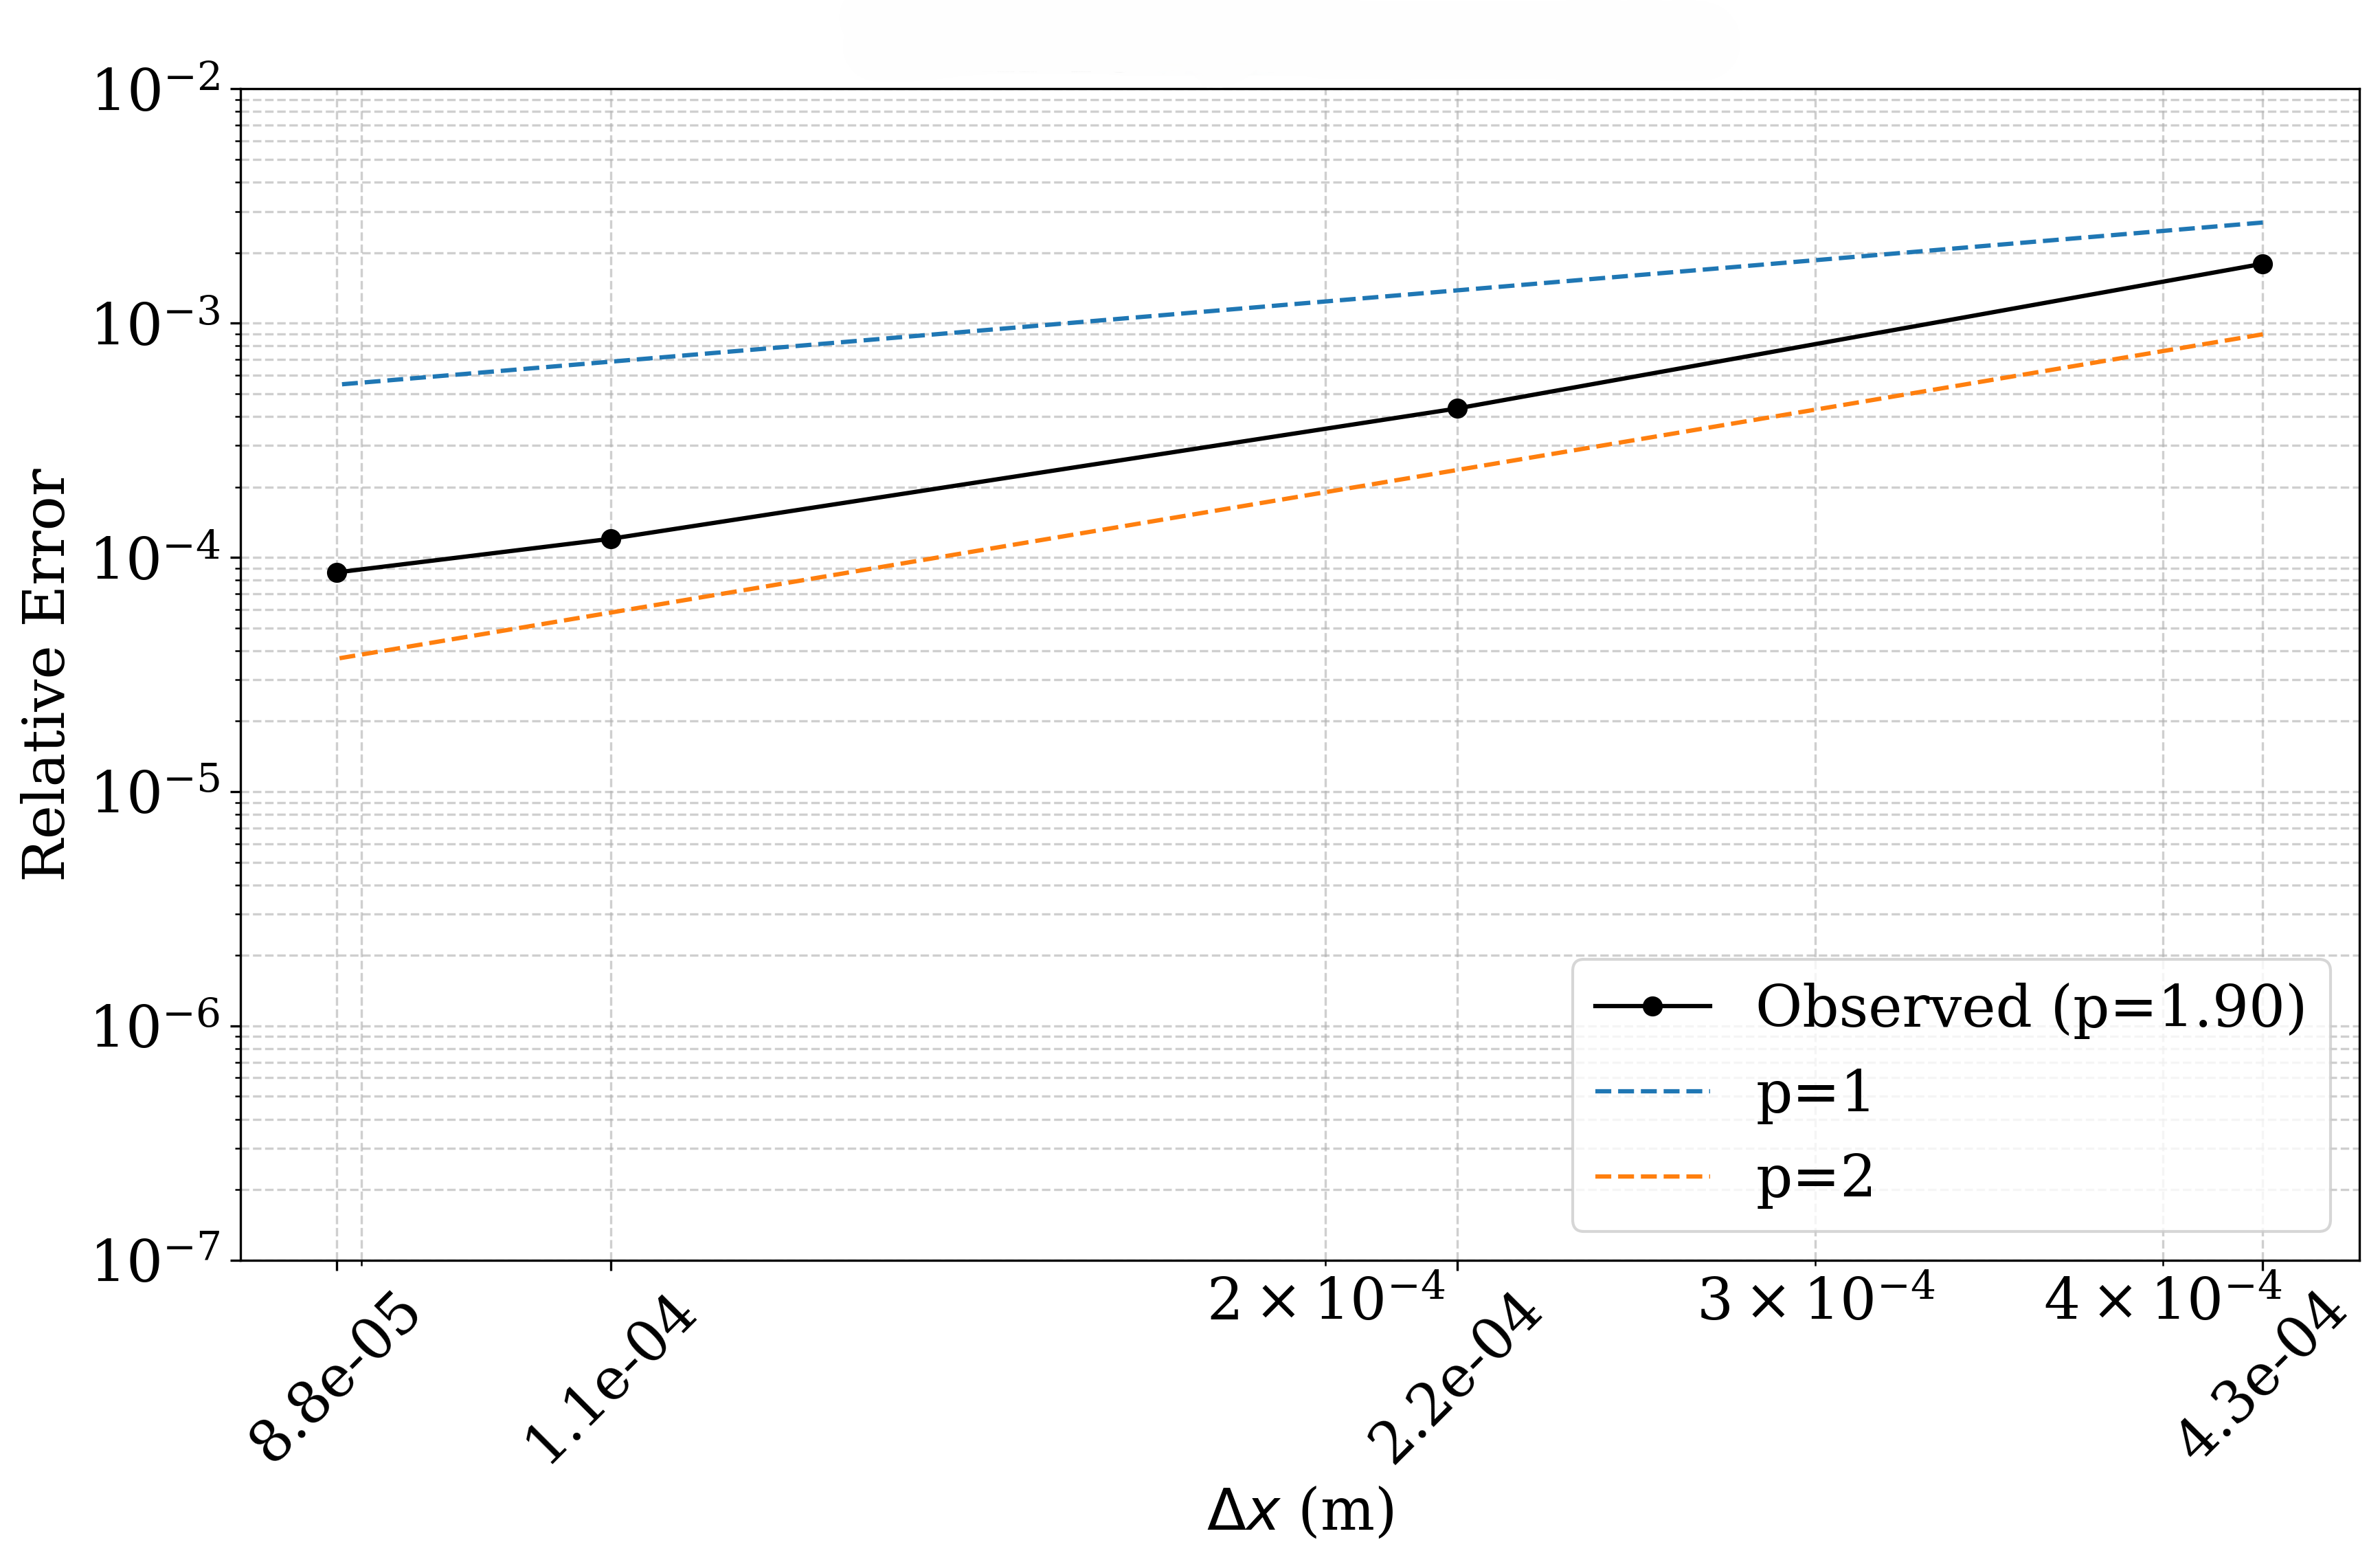
\includegraphics[width=1.0 \linewidth]{figures/code_verification/graetz/relative_err_observedP_mesh_Tbulk.png}
    \caption{Relative error in bulk temperature versus representative mesh cell size, with observed order of convergence $p = 1.90$.}
    \label{fig:tempErrs_mesh}
\end{figure}


\subsubsection{Transient Simplified EDDS}
To evaluate the coupled effects of spatial and temporal discretization, a co-refinement study was performed in which seven mesh levels (M1–M7) were paired with progressively refined time steps (T1–T7). This approach assesses how discretization errors evolve in a transient, coupled fluid-thermal system. Figure~\ref{fig:meshTimestep} shows the relative error estimated using the \texttt{StREEQ} model (Eq.~\ref{eq:streeq_model_p2}) across all mesh-timestep combinations. The error ranges from $\mathcal{O}(10^{-2})$ for coarse configurations to $\mathcal{O}(10^{-4})$ for the finest cases. A trend is observed in which error decreases with both mesh refinement and timestep reduction, indicating that spatial and temporal discretization contribute jointly to the numerical error. The relative errors show a nearly linear gradient across the mesh-timestep space, suggesting a balanced influence of spatial and temporal resolution. This behavior highlights the coupled nature of discretization error in transient simulations, where neither spatial nor temporal refinement alone is sufficient to achieve convergence.
% The coarsest combinations show substantial error accumulation after 5 seconds, while finer resolutions converge toward a consistent solution. The combination of M3 and T3 case shows less than 0.1\% error, supporting its use in downstream analysis.

\begin{figure}[htbp!]
    \centering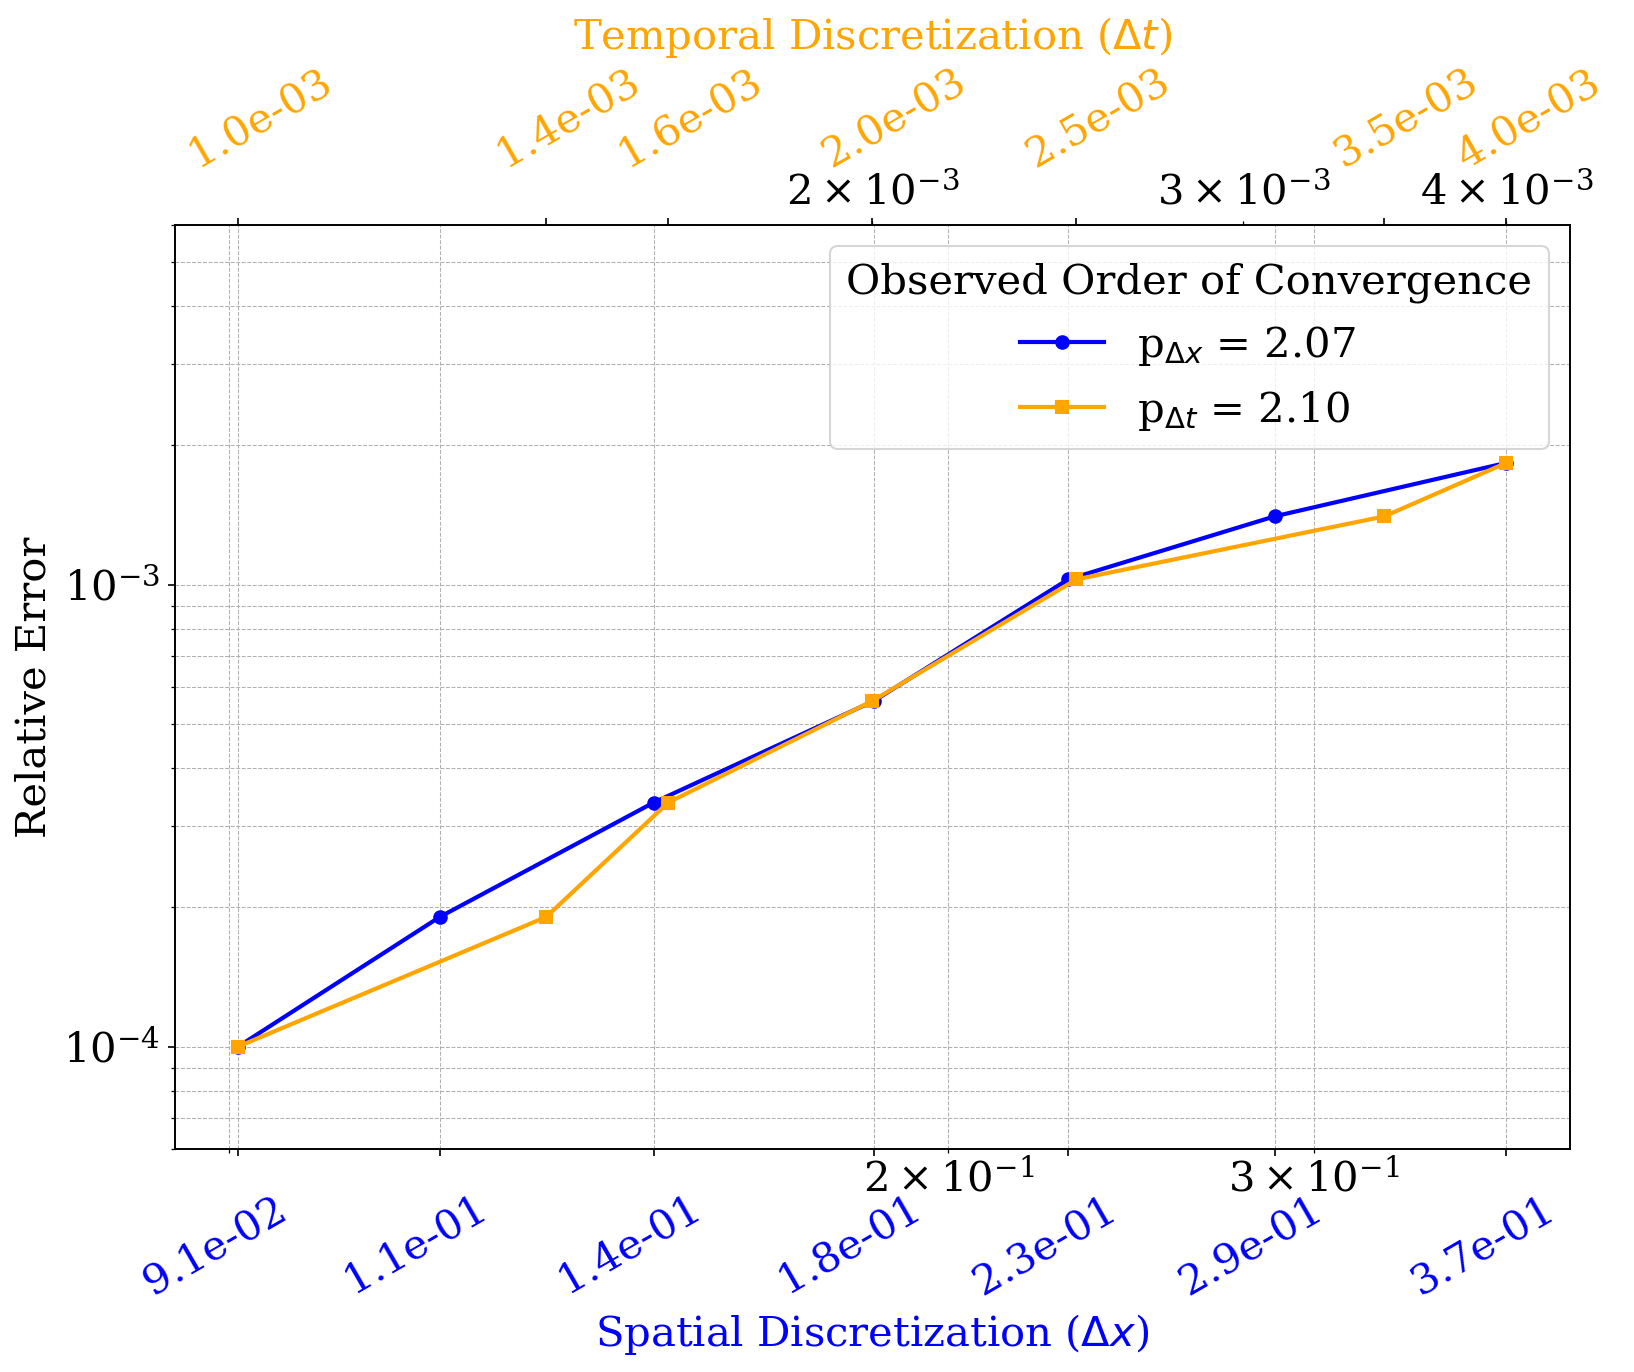
\includegraphics[width=1.0 \linewidth]{figures/solution_verification/relative_err_observedP_meshANDtimestep.png}
    \caption{Relative error across mesh-timestep combinations from the co-refinement study.}
    \label{fig:meshTimestep}
\end{figure}


\subsubsection{Solver Tolerance Study}
This study is conducted for the transient simplified EDDS configuration, where iterative solver convergence can influence the time-dependent thermal response.
To assess the impact of linear solver convergence criteria on the predicted thermal response, a solver tolerance study was conducted using mesh M3 and time step 0.005~s. Six convergence tolerances ranging from $10^{-3}$ to $10^{-8}$ were evaluated. The coarsest tolerance ($10^{-3}$) underpredicts the temperature response throughout the simulation. As the tolerance is tightened, the solutions converge toward a consistent response. The results for $10^{-7}$ and $10^{-8}$ are visually indistinguishable, indicating that solver-induced numerical error is negligible at these tolerances. Relative error was computed using the most stringent tolerance ($10^{-8}$) as the reference solution. The error decreases from $\mathcal{O}(10^{-1})$ at $10^{-3}$ to $0$ at $10^{-8}$. A tolerance of $10^{-6}$ yields a relative error below $0.0125\%$, indicating sufficient solver accuracy for this problem.

\subsubsection{Decoupled Resolution Analysis} 
To assess the impact of independently refining spatial and temporal discretization, mesh-only and timestep-only studies were performed and compared against the co-refinement results. Figure~\ref{fig:decoupledConvergence} shows that while error decreases with refinement in both cases, the observed convergence rates ($p \approx 1.06$) are significantly lower than the expected second-order behavior. This indicates that unresolved discretization error from the fixed parameter (time or space) influences the solution.

\begin{figure}[htbp!]
    \centering
    \begin{subfigure}[b]{\linewidth}
        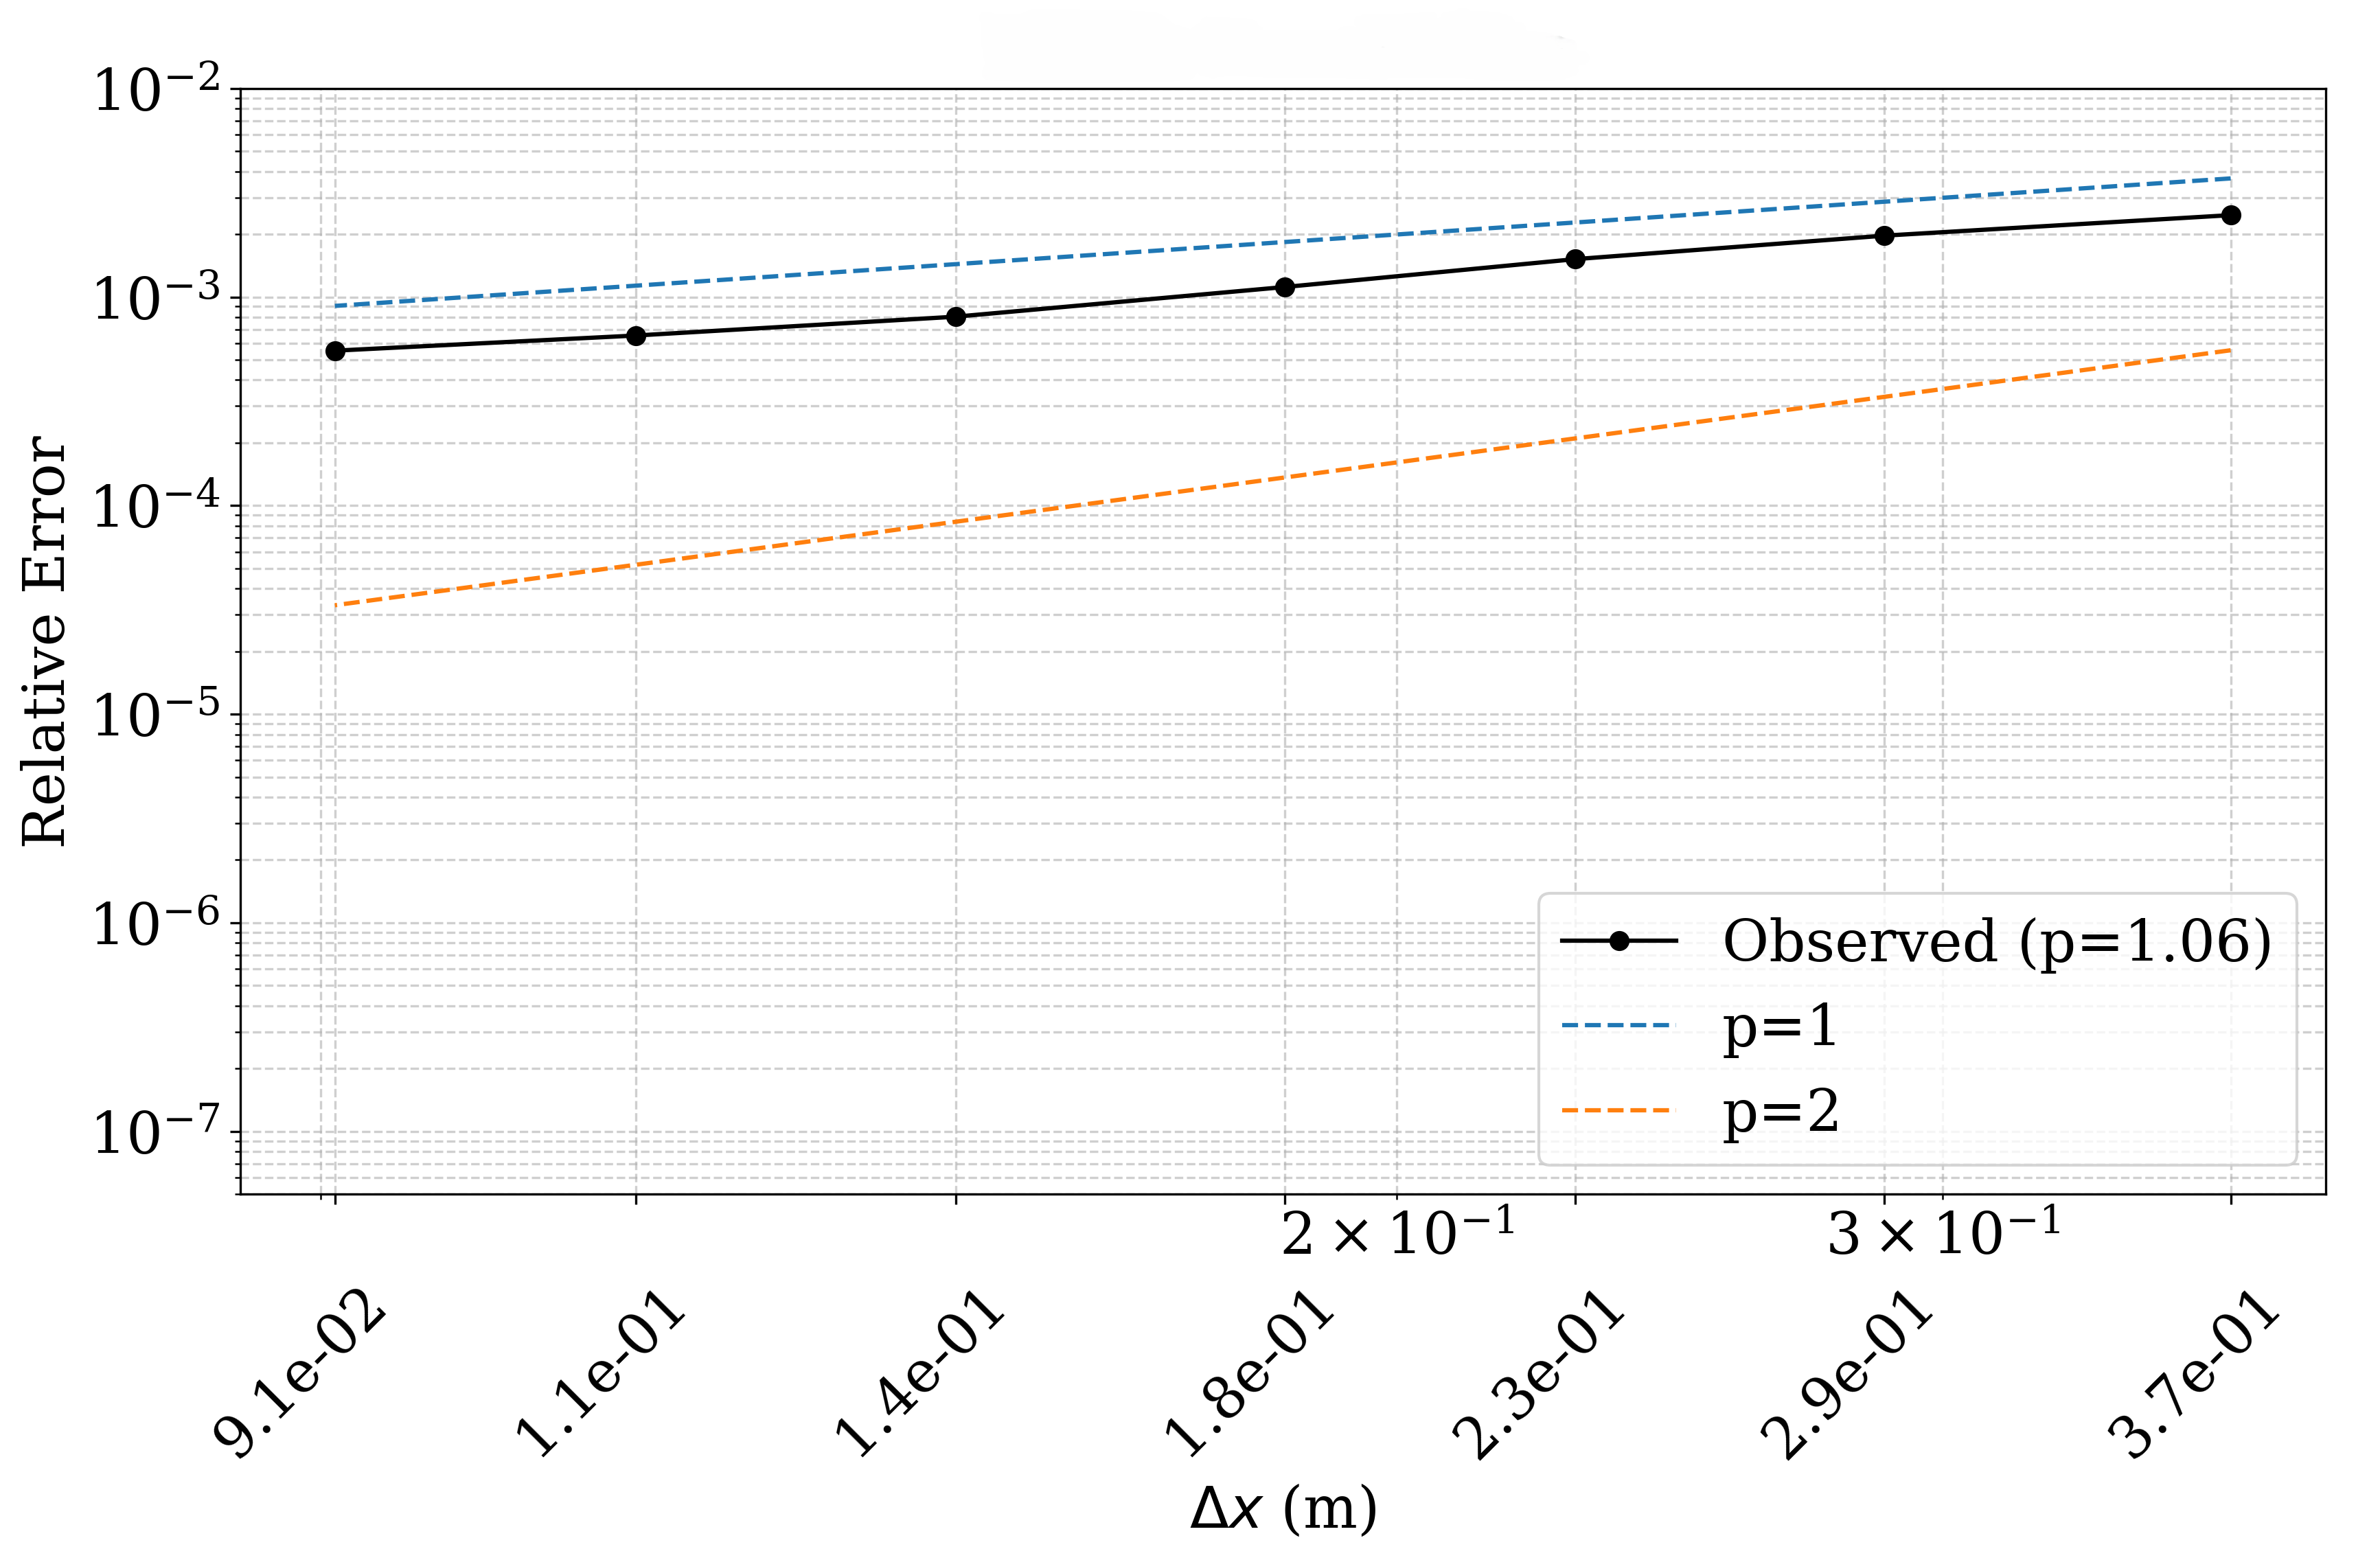
\includegraphics[width=\linewidth]{figures/solution_verification/relative_err_observedP_mesh.png}
        \caption{Mesh-only refinement (fixed timestep).}
    \end{subfigure}
    \vspace{0.5em}
    \begin{subfigure}[b]{\linewidth}
        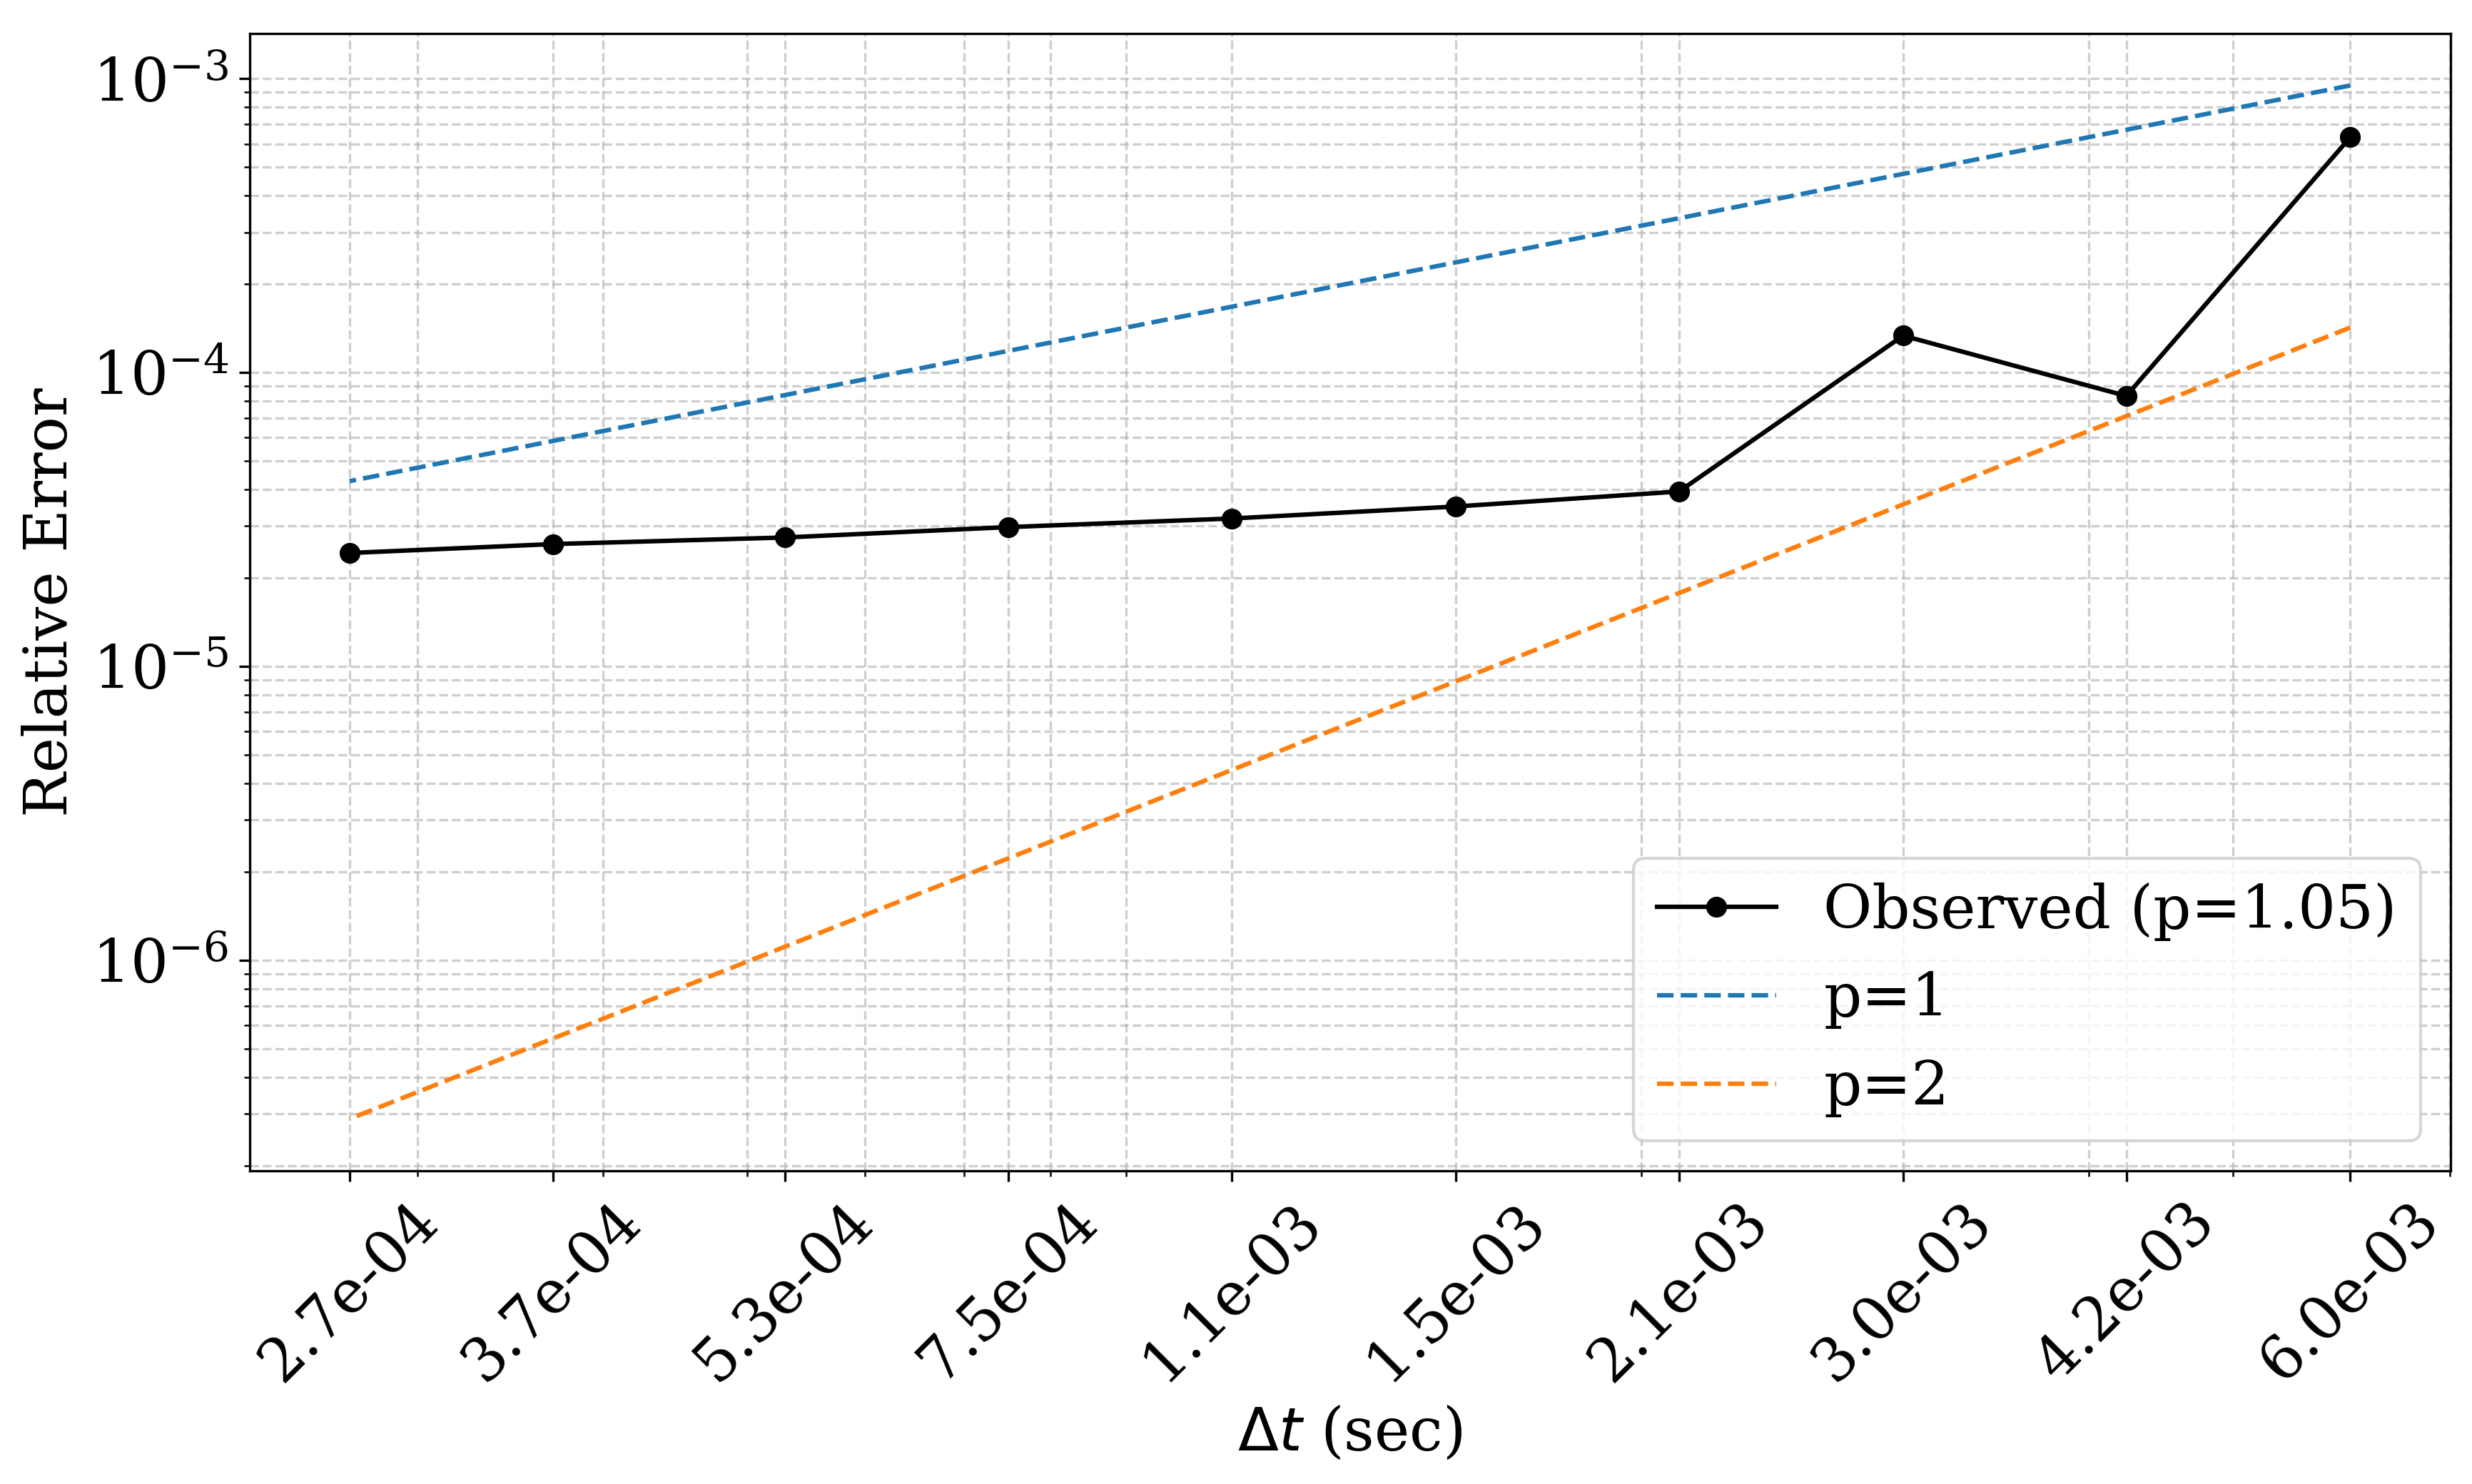
\includegraphics[width=\linewidth]{figures/solution_verification/relative_err_observedP_Tavg_z0.03_t5.png}
        \caption{Timestep-only refinement (fixed mesh).}
    \end{subfigure}
    \caption{Observed convergence behavior for independent mesh and timestep refinement studies. Both cases exhibit reduced convergence rates ($p \approx 1.06$), indicating the influence of unresolved discretization error from the fixed parameter.}
    \label{fig:decoupledConvergence}
\end{figure}

Comparison with the co-refinement results (Figure~\ref{fig:meshTimestepAll}) shows that independent refinement can under- or overestimate numerical error. In contrast, co-refinement captures the coupled influence of spatial and temporal discretization, providing a more reliable assessment of convergence behavior. These results demonstrate that independent refinement is insufficient for accurately characterizing discretization error in transient conjugate heat transfer simulations.

\begin{figure}[htbp!]
    \centering
    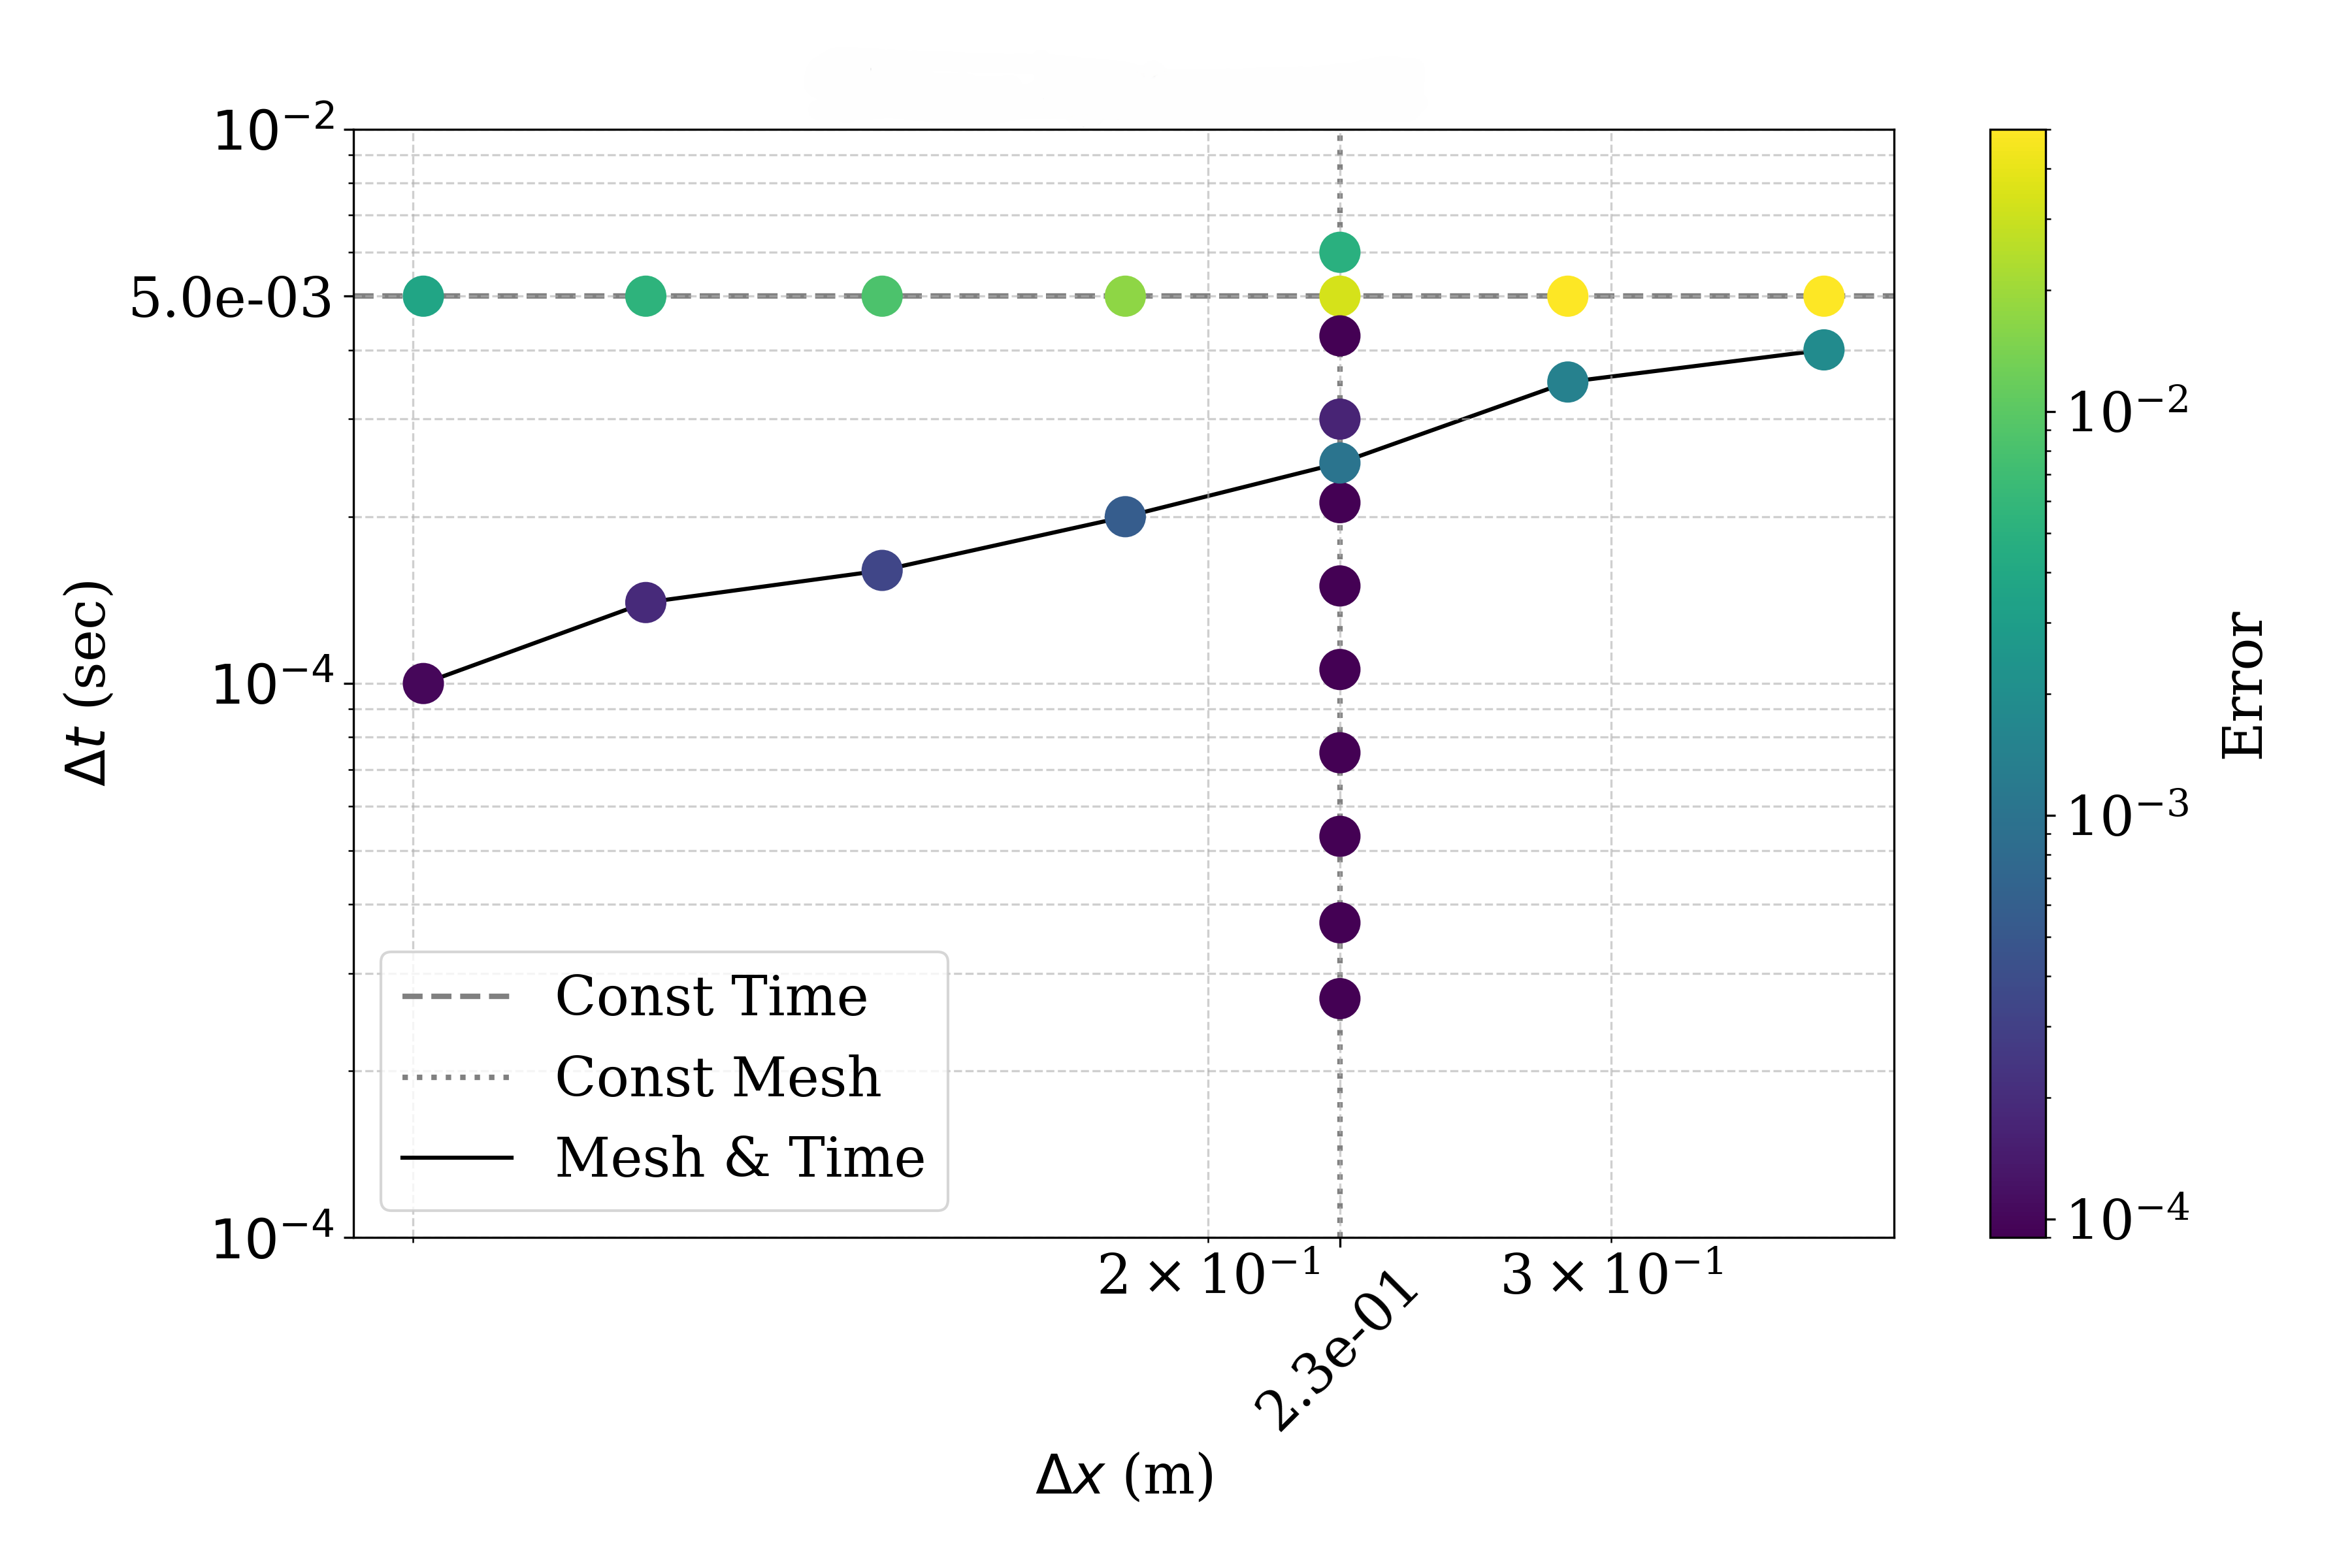
\includegraphics[width=\linewidth]{figures/solution_verification/streeq_scatter_error_Temperature_meshTime_all.png}
    \caption{Relative error across mesh and timestep combinations, including co-refined and independently refined cases.}
    \label{fig:meshTimestepAll}
\end{figure}


\subsection{Interface Energy Consistency}
To ensure that the coupled conjugate heat transfer satisfies heat-flux continuity, an additional analysis was performed on the simplified EDDS model at the fluid-solid interface with the interface discretization refining consistently with the global mesh. It is expected that the heat flux leaving the solid must equal the heat flux entering the fluid, such that $Q_{\text{solid}} + Q_{\text{fluid}} \approx 0$. The interface imbalance was defined as
\begin{equation}
\epsilon_{\text{iface}} = |Q_{\text{solid}} + Q_{\text{fluid}}|.
\label{eq:interface_imbalance}
\end{equation}
The interface energy imbalance, normalized by the applied heat source, remained on the order of $\mathcal{O}(10^{-4})$ across all mesh resolutions and did not exhibit a clear dependence on mesh refinement. Multiple competing errors, which include interface interpolation, solver tolerances, and velocity-temperature coupling, prevent the interface imbalance from decreasing with mesh refinement because the interface flux depends on temperature gradients that are highly sensitive to local discretization.

% The interface energy imbalance normalized by the applied heat source remained on the order of  $\mathcal{O}(10^{-4})$ and did not exhibit a clear dependence on mesh resolution. This indicates that the imbalance is not governed solely by spatial discretization error. This corresponds to 0.01\% of the applied heat source. Although this metric is not used as a primary discretization-error estimate, its magnitude indicates that the interface energy mismatch is negligible relative to the imposed thermal loading and is unlikely to affect the observed convergence trends in the quantities of interest. 

% This analysis was performed for both the steady-state coupled pipe model and the radial conduction model . For the radial conduction case, the interface imbalance was observed to be on the order of $\mathcal{O}(10^{-6})$. For the coupled steady-state configuration, the imbalance was on the order of $\mathcal{O}(10^{-5})$ across all mesh resolutions. For the transient simplified EDDS model the imbalance was observed to be on the order of $\mathcal{O}(10^{-4})$ . In the radial conduction case, the interface imbalance decreased with mesh refinement. In contrast, the coupled configuration did not exhibit a clear monotonic reduction in imbalance with increasing mesh resolution, although the magnitude remained small for all meshes considered.


% To ensure that the coupled conjugate heat transfer solution is physically consistent, an additional analysis was performed at the fluid–solid interface. While prior code verification studies assessed the fluid and solid physics in isolation, the coupled configuration introduces the possibility that discretization at the interface may lead to non-physical energy imbalance, even under mesh refinement. For a physically consistent solution, the heat flux leaving the solid must equal the heat flux entering the fluid at the interface, $Q_{solid} + Q_{fluid} \approx 0$. To assess this, the total heat flux on each side of the interface was computed and the interface imbalance was defined as: $\epsilon_{iface} = |Q_{solid} + Q_{fluid}|$. For the radial conduction case the difference in heat flux are on the order of magnitude of $\mathcal{O}(10^{-6})$ and for the coupled steady state case on the $\mathcal{O}(10^{-5})$. 

% Despite mesh refinement, the interface imbalance in the coupled configuration does not exhibit a clear monotonic reduction. This behavior is attributed to the presence of multiple competing error sources, including interpolation across the fluid–solid interface, solver convergence tolerances, and coupling between the velocity and temperature fields. Unlike the radial conduction case, where the error is dominated by spatial discretization, the coupled configuration introduces additional numerical errors that do not scale directly with mesh refinement. Furthermore, because the interface flux depends on temperature gradients, it is more sensitive to local discretization and interpolation errors than the primary solution variables. As a result, the interface imbalance approaches a plateau governed by solver and coupling errors rather than purely spatial resolution.

% Despite the absence of strict monotonic convergence, the magnitude of the interface imbalance remains small. This indicates that energy is well conserved across the interface and that the coupled solution is physically consistent for the purposes of this study.

\subsection{Computational Cost}
Computational cost was evaluated for the transient simplified EDDS configuration to assess the trade-off between numerical accuracy and resource requirements. Figure~\ref{fig:compCost} summarizes the cost across mesh and timestep combinations. The simulations for each of these combinations were conducted on an Intel Xeon Broadwell (BDW) E5-2695v4 at 2.1 GHz with 18 core CPU workstations. 

For the intermediate resolution case (M3 with $\Delta t = 0.0025$ s), the relative error is approximately $0.1\%$ with a computational cost of 24 minutes. Refinement to M4 with $\Delta t = 0.002$ s reduces the error to $0.055\%$, but increases computational cost to 47 minutes, corresponding to a 96\% increase in cost for a 45\% reduction in error. 

\begin{figure}[htbp!]
    \centering
    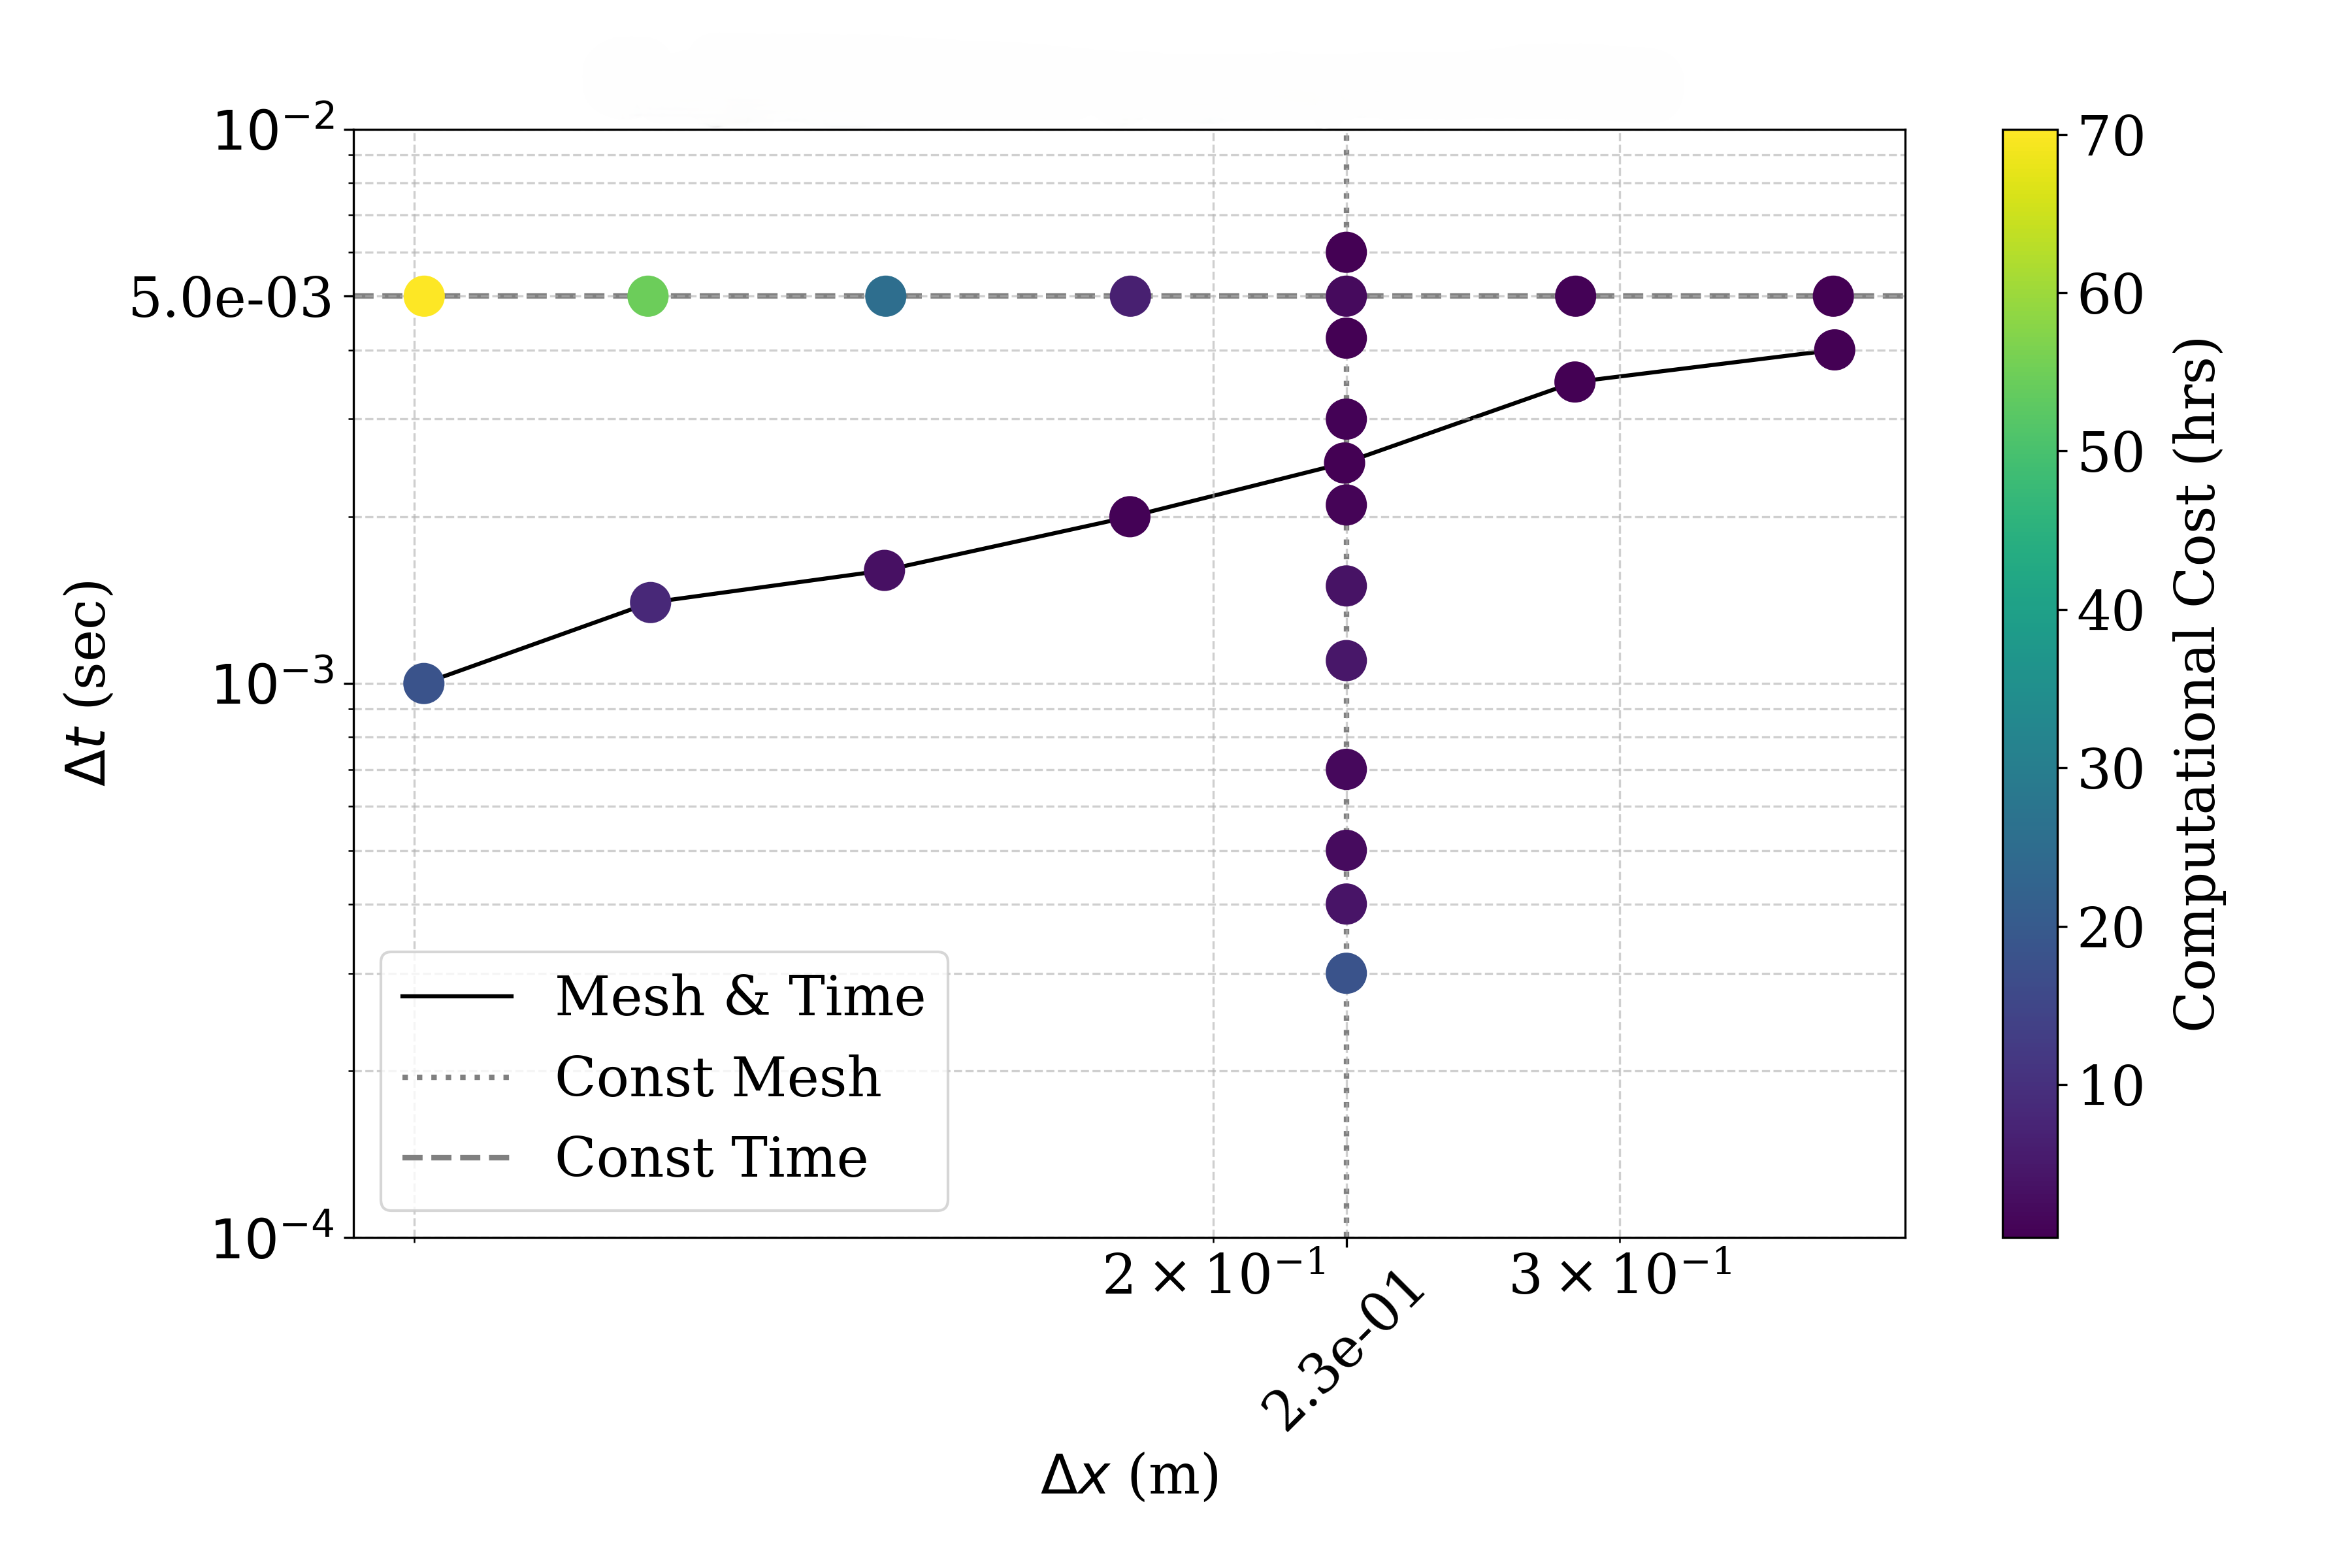
\includegraphics[width=1.0 \linewidth]{figures/solution_verification/scatter_dxdt_comCost_all.png}
    \caption{Computational Cost in hours across mesh, time step, and combined mesh time step studies. }
    \label{fig:compCost}
\end{figure}

These results demonstrate diminishing returns with increased resolution, where significant increases in computational cost yield comparatively small gains in accuracy. This trade-off highlights the importance of selecting discretization parameters that balance accuracy with computational efficiency, particularly in resource-constrained environments. Based on this analysis, the M3–T3 configuration provides a practical balance between accuracy and cost, and is selected for subsequent validation studies. This selection also supports reproducibility by enabling the study to be executed within accessible computational resources while maintaining sufficient numerical accuracy.


\section{Discussion}

% Explain Why did this happen? this indicates...
% Key Points: 
% \begin{itemize}
%     \item Key Results from the nominal model, errors and compute times why are they reasonable and acceptable.
%     \item Why we should use combined $\Delta x$ and $\Delta t$ refinement and how that limits credibility 
%     \item Why the simplified geometries for CV and SV are simple but still complex enough
%     \item Reproducibility challenges with verification: large datasets (meshes & outputs) significant computational resources to run the finer meshes  
% \end{itemize}

This study presents a rigorous verification process for a conjugate heat transfer model of a simplified medical device geometry. The objective was to establish confidence in the numerical implementation and to quantify sensitivity to spatial and temporal discretization, as well as solver convergence. These verification activities form a critical step toward building model credibility prior to validation.

Verification plays a particularly important role in medical device modeling, where experimental validation is often limited by cost, feasibility, or measurement uncertainty. In such cases, verification provides a quantitative framework to isolate numerical error, ensuring that remaining uncertainty can be attributed to physical modeling assumptions or experimental limitations rather than deficiencies in the numerical solution.

Code verification results confirm that the numerical implementation accurately represents the governing equations. The hydrodynamic case exhibited an observed order of convergence of $p = 1.90$, with errors decreasing from $\mathcal{O}(10^{-3})$ to $\mathcal{O}(10^{-5})$, while the radial conduction case achieved $p = 2.08$, consistent with second-order spatial accuracy. These results demonstrate that both the momentum and energy equations are correctly discretized and solved under idealized conditions.

The verification process was intentionally structured to progressively isolate the governing physics relevant to the final coupled transient configuration. The hydrodynamic verification case isolated the momentum equations and confirmed accurate velocity-field discretization independent of thermal effects. The radial conduction case then isolated steady-state thermal transport within the solid domain by removing fluid effects through an adiabatic interface boundary condition. While these studies independently verified the momentum and thermal governing equations, neither configuration evaluated transient thermal transport or the thermal coupling behavior at the fluid-solid interface. To bridge this gap, a transient thermal diffusion verification case was introduced by imposing zero velocity throughout the fluid region, reducing the governing energy equation to a pure diffusion problem with an analytical Bessel-function solution. This intermediate verification configuration enabled assessment of transient thermal transport behavior independently of advection while also verifying that the transient solid temperature response was correctly imposed across the fluid-solid interface into the fluid region. The transient diffusion study demonstrated near second-order spatial convergence, with observed orders ranging from $p=2.15$ to $p=2.47$ across multiple transient times.

Solution verification results highlight the importance of evaluating discretization error in coupled, application-relevant configurations. In the transient simplified EDDS case, co-refined mesh and timestep studies revealed that spatial and temporal discretization errors interact and accumulate over time. Independent refinement of either parameter produced reduced convergence rates ($p \approx 1.06$), indicating that unresolved error from the fixed parameter influences the solution. This demonstrates that accurate error estimation in transient multiphysics simulations requires consistent co-refinement of spatial and temporal discretization. 

The interface energy consistency results support the coupled solution. The interface heat flux is more sensitive to local discretization since it does not exhibit monotonic convergence with mesh refinement. The imbalance remains small, approximately $0.01\%$ of the applied heat source, indicating that energy is well conserved across the interface. This imbalance is reasonable so long as it remains smaller than the discretization error.


% % Add this but edit cause it's too long for interface analysis:
% The absence of monotonic reduction in the normalized interface imbalance is not unexpected for the coupled conjugate heat transfer case. Unlike the isolated radial conduction verification problem, the coupled case introduces additional numerical error sources, including interface interpolation between separate fluid and solid regions, gradient reconstruction used to compute heat flux, pressure--velocity--temperature coupling, and finite solver tolerances. Because the imbalance is computed from integrated derived quantities rather than primary solution variables, it can be more sensitive to these effects and may plateau once spatial discretization error becomes smaller than the coupling and linear-solver error floor. 
% %%%%%%%%%%%%%%%%%%%%%%%%%%%%%%%

% The differing convergence behavior between the radial conduction and coupled configurations highlights the role of additional numerical error sources introduced by conjugate heat transfer coupling. In the radial conduction case, the interface imbalance is primarily governed by spatial discretization error and exhibits the expected reduction with mesh refinement. 

% In contrast, the coupled configuration introduces competing error sources, including interpolation across the fluid–solid interface, solver convergence tolerances, and coupling between the velocity and temperature fields. These errors do not scale directly with mesh refinement and can dominate the interface flux balance. Additionally, because the interface heat flux depends on temperature gradients, it is more sensitive to local discretization and interpolation errors than the primary solution variables. As a result, the interface imbalance approaches a plateau rather than exhibiting strict monotonic convergence.


The computational cost analysis further emphasizes the practical implications of verification. While refinement improves accuracy, diminishing returns are observed as computational cost increases. Importantly, the relationship between discretization parameters and computational cost is not strictly monotonic. Larger timesteps or coarser meshes do not always yield lower runtime due to increased solver iterations and numerical stiffness. This highlights the need to evaluate computational cost based on measured runtime rather than assuming a direct relationship with discretization parameters.

The selected M3–T3 configuration provides a balance between accuracy (relative error $\sim 0.1\%$) and computational cost (24 minutes), making it suitable for downstream validation studies. This choice reflects a risk-informed approach to modeling, where sufficient accuracy is achieved without exceeding practical computational constraints. If stricter error tolerances are required for a given application, further refinement can be applied; however, this will incur increased computational cost and should be justified based on the sensitivity of the decision-making context.

Geometric simplification was essential to enable rigorous verification while retaining the dominant physics of the system. Although detailed device features such as coil geometry and the expanding mouthpiece were excluded, the simplified model captures the key fluid and thermal transport behavior governing the system response. This level of abstraction allows verification to be performed under controlled conditions while maintaining relevance to the physical system. More complex geometric features can be reintroduced during validation without compromising the credibility established through verification.

Finally, this study highlights the role of reproducibility in verification. High-fidelity simulations require large datasets and substantial computational resources, particularly for fine mesh and timestep combinations. By implementing scripted workflows and providing publicly accessible computational artifacts, this work ensures that verification results are traceable, reproducible, and accessible. This is particularly important in settings where computational resources are limited, as it enables broader use and independent assessment of the modeling approach. This verification process establishes a credible foundation for subsequent validation and application of the model within the ASME V\&V 40 framework. 

This work is intentionally scoped to verification in order to isolate and quantify numerical error prior to introducing additional sources of uncertainty. While uncertainty quantification and validation are essential components of the full VVUQ process, combining all elements within a single study can obscure the attribution of error sources. By separating verification from validation and uncertainty quantification, this work establishes a controlled and transparent foundation for subsequent analysis. A companion study will extend this work to include validation and uncertainty quantification under application-relevant conditions.


\section{Conclusion}
This study represents the first step in a comprehensive credibility assessment for a computational model of a simplified medical device geometry involving conjugate heat transfer. Using \texttt{OpenFOAM}'s \texttt{chtMultiRegionFoam} solver, a rigorous verification effort was conducted, including both code and solution verification, to evaluate numerical accuracy and implementation. 

The results demonstrate that the solver reliably captures laminar flow and heat transfer behavior, with discretization errors from spatial resolution, timestep size, and solver tolerance systematically reduced to acceptable levels. Importantly, this study shows that the choice of resolution directly impacts both numerical accuracy and computational cost, requiring a careful balance between the two. A key finding is that spatial and temporal discretization errors in transient coupled simulations cannot be assessed independently. Co-refinement of mesh and timestep is necessary to obtain reliable estimates of numerical error, while independent refinement can lead to misleading convergence behavior. This highlights the importance of consistent and systematic verification practices when evaluating multiphysics models. The use of a simplified geometry enabled rigorous verification while preserving the dominant fluid and thermal transport physics of the device. This approach demonstrates that meaningful verification can be achieved even when analytical solutions are limited and full system complexity is not yet incorporated. 

The interface energy consistency analysis further supports the coupled solution. The interface imbalance did not exhibit monotonic convergence with mesh refinement, it remained small, approximately $\mathcal{O}(10^{-4})$ of the applied heat source, thus the energy is well conserved across the fluid–solid interface and that the observed convergence behavior is not associated with a non-physical coupling error. This work also emphasizes practical considerations in verification, including computational cost and reproducibility. High-fidelity simulations require significant resources and generate large datasets, particularly for fine mesh and timestep combinations. By identifying an efficient resolution strategy and providing reproducible workflows and publicly accessible artifacts, this study supports broader accessibility and transparency in computational modeling.

This study is aligned with the ASME V\&V 40 framework and contributes a reproducible, risk-informed case study for building model credibility in medical device applications. For the medium–low risk context considered here, the verification approach demonstrates that a level of rigor beyond minimal practice can be achieved through targeted model simplification and systematic analysis. Establishing numerical correctness and quantifying discretization error provides a critical foundation for subsequent validation and uncertainty quantification efforts. Future work will build upon this verification foundation by incorporating validation and uncertainty quantification to complete the full VVUQ framework. Overall, this work demonstrates that systematic verification of coupled fluid–thermal models, even in the absence of analytical solutions for the full system, can provide credible and decision-relevant modeling evidence under practical computational constraints. 

%%%%%%%%%%%%%%%%%%%%%%%%%%%%%%%%%%%%%%%%%%%%%%%%%%%%%%%%%%%%%%%%%%%%%%
\section*{Acknowledgment} %% ASME requests this exact spelling, singular.
The authors gratefully acknowledge support from the U.S. Department of Energy’s Computational Science Graduate Fellowship (DOE CSGF) under contract number DE-SC0022158, as well as support and mentoring from Sandia National Laboratories. 


%%%%%%%%%%%%%%%%%%%%%%%%%%%%%%%%%%%%%%%%%%%%%%%%%%%%%%%%%%%%%%%%%%%%%%
\section*{Funding Data}
Sandia National Laboratories is a multimission laboratory managed and operated by National Technology \& Engineering Solutions of Sandia, LLC, a wholly owned subsidiary of Honeywell International Inc., for the U.S. Department of Energy’s National Nuclear Security Administration under contract DE-NA0003525.

This paper describes objective technical results and analysis. Any subjective views or opinions that might be expressed in the paper do not necessarily represent the views of the U.S. Department of Energy or the United States Government.

U.S.\ Department of Energy, Computational Science Graduate Fellowship, DE-SC0022158. 


%%%%%%%%%  NOMENCLATURE  %%%%%%%%%%%%%%%%%%%%%%%%%%%%%%%%%%%%%%%%%%%%%
%% \section{Nomenclature}
%% %% Name of nomenclature can be changed using an optional argument to the environment.
%%
%% \EntryHeading{Greek Letters}
%% \entry{symbol}{definition}
%%
%% Must run latex twice to align the columns.

% \begin{nomenclature}

% \entry{$\overline{h}$}{average heat transfer coefficient (W m$^{-2}$ K$^{-1}$)}
% \entry{$k$}{thermal conductivity (W m$^{-1}$ K$^{-1}$)}
% \entry{$\mathbf{q}$}{heat flux vector (W m$^{-2}$)}

% \EntryHeading{Greek Letters}
% \entry{$\alpha$}{thermal diffusivity (m$^2$ s$^{-1}$)}
% \entry{$\nu$}{kinematic viscosity (m$^2$ s$^{-1}$)}

% \EntryHeading{Dimensionless Groups}
% \entry{Pr}{Prandtl number, $\nu/\alpha$}
% \entry{Sc}{Schmidt number, $\nu/\mathcal{D}_{1,2}$}

% \EntryHeading{Superscripts and Subscripts}
% \entry{b}{bulk value}
% \entry{$\infty$}{free stream value}

% \end{nomenclature}

%%%%%%%%%%%%%  BIBLIOGRAPHY  %%%%%%%%%%%%%%%%%%%%%%%%%%%%%%%%%%%%%%%%%

\nocite{*} %% <=== delete this line - unless you wish to typeset the entire contents of your .bib file.

\bibliographystyle{asmejour}   %% .bst file that follows ASME journal format. Do not change.

\bibliography{references} %% <=== change this to name of your bib file

%%%%%%%%%%%%%%%%%%%%%%%%%%%%%%%%%%%%%%%%%%%%%%%%%%%%%%%%%%%%%%%%%%%%%%

%%%%%%%%%%%%%%%  APPENDICES  %%%%%%%%%%%%%%%%%%%%%%%%%%%%%%%%%%%%%%%%%

%% Note that appendices will be "numbered" A, B, C, ... etc. Use \section, not \section*
%% Subsections need not be numbered, use \subsection*
%% The equation counter is reset for each appendix
%% Figures will be numbered consecutively

% \appendix   %%% starting appendices
% 
%%%%%%%%%%%%%%%%%%%%%%%%%%%%%%%%%%%%%%%%%%%%%%%%%%%%%%%%%%%%%%%%%%%%%%
\section{Risk Informed Credibility Plan }

As outlined in ASME V\&V 40, a risk-informed approach to model credibility requires clear definition of the question of interest, context of use, and associated model risk. These three elements guide the rigor required for each credibility activity.

\paragraph{Question of Interest:} What are the potential bioeffects resulting from chemical deposition onto the oral mucosa in users of an Electronic Drug Delivery System (EDDS)?

\paragraph{Context of Use:} A fluid and heat transfer model is used to characterize the velocity and temperature distribution within representative mouth cavity geometries of EDDS users. This information supports downstream chemical transport and deposition modeling.

\paragraph{Risk Assessment:} The model is assessed as having **low influence** on decision-making and a **moderate consequence** if incorrect. Based on the ASME V\&V 40 framework, this places the overall model risk between low and moderate (see Figure~\ref{fig:riskAssessment}).

\begin{figure}[H]
    \centering
    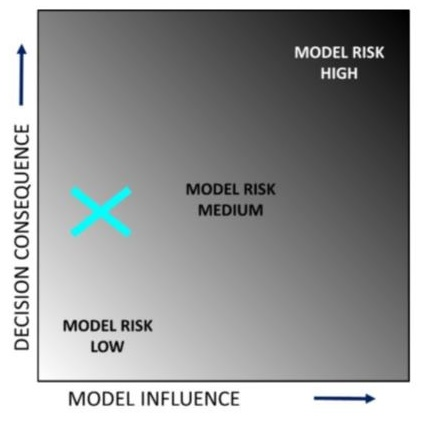
\includegraphics[width=0.5\linewidth]{figures/schematic/risk_assessment.jpg}
    \caption{Model risk classification based on decision consequence and model influence, as defined in ASME V\&V 40 \cite{vv40}.}
    \label{fig:riskAssessment}
\end{figure}

Based on this risk assessment, the required level of rigor for each credibility activity (e.g., verification, validation, uncertainty quantification) can be determined. Figure~\ref{fig:credibilityvvuq} shows the credibility activities aligned with the level of rigor gradations.

\begin{figure}[H]
    \centering
    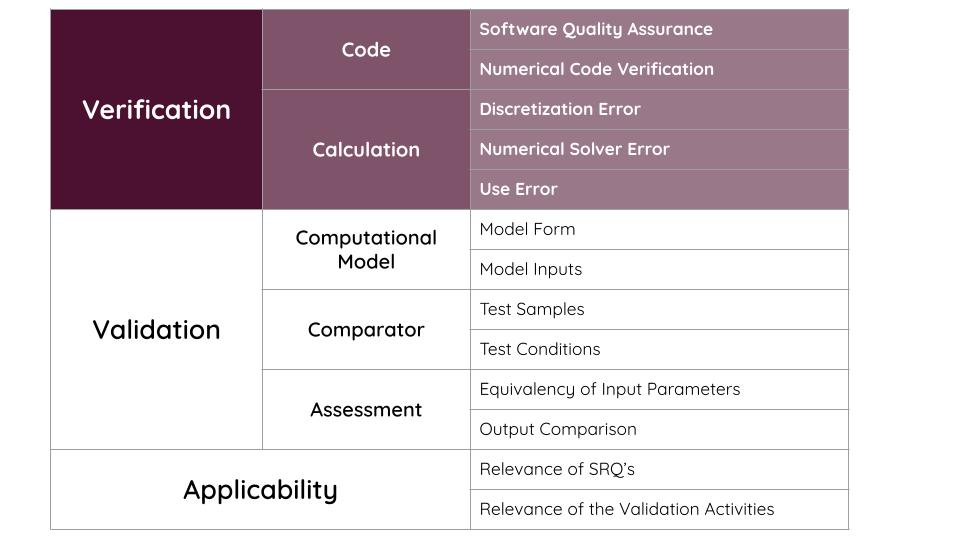
\includegraphics[width=0.8\linewidth]{figures/schematic/vvuq_workflow.jpg}
    \caption{Credibility activities and recommended rigor gradations based on model risk, following ASME V\&V 40 \cite{vv40}.}
    \label{fig:credibilityvvuq}
\end{figure}

%% To omit final list of figures and tables, use the class option [nolists]
\end{document}
 